\RequirePackage{silence}
\WarningFilter{latexfont}{Font shape `TU/}
\WarningFilter{latexfont}{Size substitutions}
\RequirePackage[warnings-off={mathtools-colon,mathtools-overbracket}]{unicode-math}
% Ошибки ^
\documentclass[fleqn]{article}
\usepackage{amsmath,nccmath} % Математика
\usepackage[a5paper, margin=12mm]{geometry}
% Пакеты
\usepackage{polyglossia} % Язык
\setmainlanguage{russian}
\setotherlanguage{english}
\setkeys{russian}{babelshorthands=true}
\usepackage{fontspec} % Шрифты .otf
\usepackage{titlesec} % Заголовки
\usepackage{tabularx,multicol,multirow,array,makecell} % Таблицы
\usepackage{enumitem} % Списки
\usepackage{graphicx,float} % Графика
\usepackage{xcolor} % Цвет
\usepackage{empheq}
\usepackage[makeroom]{cancel}
\usepackage[most]{tcolorbox} % Удобные рамки
\usepackage[open,openlevel=1]{bookmark} % Секции в pdf-файле
\graphicspath{{svg/}}
% Нумерация
\pagenumbering{gobble} % Страницы
\setcounter{secnumdepth}{0} % Заголовки
% Шрифты
\setmainfont[SizeFeatures={Size=12}]{Century Schoolbook}
\setmathfont[Scale=1.2]{TeX Gyre Schola Math}
\newfontfamily\bold[SizeFeatures={Size=12}]{Century Schoolbook Bold}
\newfontfamily\ital[SizeFeatures={Size=12}]{Century Schoolbook Italic}
\newfontfamily\boldital[SizeFeatures={Size=12}]{Century Schoolbook Bold Italic}
\newfontfamily\gilroysub[SizeFeatures={Size=16},UprightFont={*-Medium}]{Gilroy}
\newfontfamily\gilroy[SizeFeatures={Size=19},UprightFont={*-UltraLight}]{Gilroy}
\newfontfamily\tinyt[SizeFeatures={Size=10}]{Century Schoolbook}
% Стили
\titleformat*{\subsection}{\raggedright\gilroysub}
\titleformat*{\section}{\gilroy\centering}
\titlespacing*{\subsection}{0pt}{6pt}{0pt}
\titlespacing*{\section}{0pt}{6pt}{1pt}
\definecolor{desc}{HTML}{888888}
\definecolor{table}{HTML}{D9D9D9}
\newcommand{\modb}[1]{\ \left(\mathrm{mod}\ #1\right)}
\newcommand{\modn}[1]{\ \mathrm{mod}\ #1}
\newcommand{\qedb}{\ \char"25A0}
\newcommand{\qedw}{\ \char"25A1}
\newcommand{\id}[1]{\text{id}_{#1}}
\newcommand{\norm}[1]{\lVert#1\rVert}
\newcommand{\abs}[1]{\left|#1\right|}
\newcommand{\sgnb}[1]{\text{sgn}\hspace*{-2pt}\left(#1\right)}
\newcommand{\sgnn}[1]{\text{sgn}\ #1}
\newcommand{\ren}[1]{\Re\text{e}\ #1}
\newcommand{\reb}[1]{\Re\text{e}\left(#1\right)}
\newcommand{\imn}[1]{\Im\text{m}\ #1}
\newcommand{\imb}[1]{\Im\text{m}\left(#1\right)}
\newcommand{\optm}[1]{\underset{\scriptscriptstyle #1}{\text{opt}}}
\newcommand{\optl}[1]{\text{opt}_{#1}}
\newcommand{\diff}{\text{d}}
\newcommand{\footnotes}[2]{$^{#1}$\hspace*{-1.1pt}\let\thefootnote\relax\footnote
{\hspace*{-18pt}#1 #2}}
\newcommand{\multiset}[2]{\left(\!\!\binom{#1}{#2}\!\!\right)}
\newcommand{\stirl}{\genfrac\{\}{0pt}{}}

% Смена шрифта для \mathcal
\DeclareMathAlphabet{\mathcal}{OMS}{cmsy}{m}{n}
\SetMathAlphabet{\mathcal}{bold}{OMS}{cmsy}{b}{n}

% Понижает высоту степени тригонометрических функций
\newcommand{\trsp}{\hspace*{-2.3pt}\phantom{}}

% Minipage environment
\newenvironment{column*}[2]{
\begin{minipage}[#1]{#2}
\setlength\baselineskip{13.4pt} % Строка
\setlength{\parskip}{6pt} % Абзац
\abovedisplayskip=6pt % Формула над
\belowdisplayskip=6pt % Формула под
\raggedright % Выравнивание
}{\end{minipage}}

% Tabular environment
\def\center{c}

\newenvironment{tabularc}[4]{
\if\center #4
\centering
\fi
\setlength\tabcolsep{#1}
\setlength\extrarowheight{#2}
\begin{tabular}{#3}
}{\end{tabular}\par}

% Tabularx environment
\newenvironment{tabularcx}[4]{
\setlength\tabcolsep{#1}
\setlength\extrarowheight{#2}
\tabularx{#4}{#3}
}{\endtabularx\par}

\newcolumntype{L}{>{\raggedright\arraybackslash}X}
\newcolumntype{R}{>{\raggedleft\arraybackslash}X}
\newcolumntype{C}{>{\centering\arraybackslash}X}

% Square cases environment
\makeatletter\newenvironment{sqcases}{%
  \matrix@check\sqcases\env@sqcases
}{%
  \endarray\right.%
}
\def\env@sqcases{%
  \let\@ifnextchar\new@ifnextchar
  \left\lbrack
  \def\arraystretch{1.2}%
  \array{@{}l@{\quad}l@{}}%
}\makeatother

% Theorem Tcolorbox
\newtcolorbox{theorem}{
enhanced,
boxrule=0mm,frame hidden,arc=0mm,
colback=white!0,
boxsep=0mm,left=3.5mm,
borderline west={2pt}{0pt}{black},
before skip=6pt,after skip=7pt
}


\begin{document}

% indentation
\setlength\baselineskip{13.4pt} 
\setlength\parskip{6pt}
\setlength\parindent{0pt}
\abovedisplayskip=6pt % displaymath
\belowdisplayskip=6pt % displaymath
\raggedright          % forced linebreaks

\section{Элементарная теория чисел}
\subsection{Делимость}
Пусть $a,b\in\mathbb{Z}$. Тогда {\ital a} --- {\bold делитель} {\ital b}, когда
$$ax=b,\ x\in\mathbb{Z}\iff a\mid b\iff \lvert a\rvert\leq\lvert b\rvert$$
% ---
Отношение делимости {\ital транзитивно}, такое выражение можно {\ital перемножить}
с другим:
$$
\times\begin{cases}
\begin{aligned}
a&\mid b\\
c&\mid d
\end{aligned}
\end{cases}
\hspace*{-12pt}\implies
ac\mid bd
$$
% ---
Общий делитель чисел делит их {\ital линейную комбинацию}:
$$a\mid b,c\implies a\mid bx+cy,\quad x,y\in\mathbb{Z}$$
% ---
Заметим, что $a=bx+cy$\footnotes{*}{Такое уравнение называют {\ital соотношением Безу}, а
{\ital x} и {\ital y} --- {\ital коэффициентами Безу {\color{desc}(Э. Безу)}}.},
когда $(b,c)\mid a$.\par

{\bold Доказательство.} Пусть $d:=(b,c)$, тогда:
$$d\mid b,c\implies d\mid(bx+cy)\implies d\mid a\qedb$$
% ---
Коэффициенты Безу $(x,y)$ {\ital неуникальны} и легко выражаются
{\ital\color[HTML]{888888}(доказывается подстановкой в соотношение)}:
$$(x+mk,y-ak),\ k\in\mathbb{Z}$$

\newpage
\subsection{Наибольший общий делитель}

{\ital Наибольший общий делитель}\footnotes{*}{Сокращённо {\ital НОД}, или {\ital Greatest Common Divisor} ({\ital GCD}).} для $\{a_k\}_{k\in\mathbb{N}}$ --- такое $gcd(\{a_k\})$, что
% ---
$$\exists d\colon d\mid gcd(\{a_k\})\mid\{a_k\}.$$
% ---
Упрощённая запись $gcd(\{a_k\})=(\{a_k\})$.

Этот бинарный оператор {\ital коммутативен}, {\ital ассоциативен}\\ и {\ital дистрибутивен}.

\subsection{Наименьшее общее кратное}

{\ital Наименьшее общее кратное}\footnotes{**}{Сокращённо {\ital НОК}, или {\ital Least Common Multiple} ({\ital LCM}).} для $\{a_k\}_{k\in\mathbb{N}}$ --- такое $lcm(\{a_k\})$, что
% ---
$$\exists m\colon \{a_k\}\mid lcm(\{a_k\})\mid m.$$
% ---
Упрощённая запись $lcm(\{a_k\})=[\{a_k\}]$.

Этот бинарный оператор {\ital коммутативен} и {\ital ассоциативен}, однако {\ital не дистрибутивен}.

\subsection{Двойственность}

НОД и НОК {\ital двойственны} друг другу:
% ---
$$(a,b)\cdot[a,b]=ab$$
% ---
{\bold Доказательство.} Пусть $m:=[a,b]$, тогда:
% ---
$$a,b\mid m\iff ab\mid am,bm\iff ab\mid (am,bm)\iff ab\mid (a,b)m$$
% ---
Так как $(a,b)\mid [a,b]\mid ab$, то $ab/(a,b)\mid [a,b]$.

Значит, $ab/(a,b)\leq [a,b]$. Но $[a,b]$ --- {\ital наименьшее} общее кратное $a,b$. Следовательно, $ab/(a,b)\nless [a,b]$, поэтому:
% ---
$$ab/(a,b)=[a,b]\iff ab=(a,b)\cdot [a,b]\qedb$$

\section{Элементарная алгебра}

% Вспомнить о понятии окрестности точки,
% функции расстояния --- метрики (см. п. 5)

\subsection{Свойства неравенств}

Отношение сравнения {\ital транзитивно}; неравенства можно {\ital складывать}
{\ital\color{desc}(не вычитать)}, а также {\ital перемножать} и возво"=дить
в натуральную степень $k$ {\ital\color{desc}(без смены знака)}:
% ---
$$
\begin{cases}
a\less b\\
c\leq d
\end{cases}\hspace*{-12pt}\implies
\begin{cases}
a + c\less b + d\\
ac\less bd\\
a^k\less b^k
\end{cases}
$$
% ---
При умножении на отрицательное число $m$ знак неравенства {\ital инвертируется}:
% ---
$$a\less b\iff am\greater bm$$

\subsection{Неравенство Коши}

Пусть $a,b\in \mathbb{R}^+$. Тогда верно {\ital\color{desc}(О.Л. Коши)}:
% ---
$$\frac{a+b}{2}\geq \sqrt{ab}$$
% ---
{\bold Доказательство.}
$$\frac{a+b}{2}\geq \sqrt{ab}\iff a+b\geq 2\sqrt{ab}\iff a-2\sqrt{ab}+b\geq 0\iff$$
\\[-11pt]
$$(\sqrt{a}-\sqrt{b})^2\geq 0\qedb$$

\subsection{Неравенство Бернулли}

Пусть $n\geq 2,\ x\greater 0$. Тогда верно {\ital\color{desc}(Я. Бернулли)}:
% ---
$$(1+x)^n\greater 1+nx$$
% ---
{\bold Доказательство.} Проверим базис индукции $n=2$:
% ---
$$(1+x)^2\greater 1+2x\iff 1+2x+x^2\greater 1+2x\qedw$$
% ---
Проверим индукционный шаг $n+1$. Пусть утверждение верно для некоторого
$n\greater 2$, тогда:
% ---
$$(1+x)^n\greater 1+nx\iff (1+x)^{n+1}\greater (1+nx)(1+x)\iff$$
$$(1+x)^{n+1}\greater 1+(n+1)x+nx^2\iff (1+x)^{n+1}\greater 1+(n+1)x\qedb$$

\subsection{Свойства функций}

Функция $f$ {\ital возрастает}, когда
% ---
$$\forall x_1,x_2\in D_f,\ x_1\less x_2\implies f(x_1)\less f(x_2).$$
% ---
{\ital Максимумом} функции $f$ называется такая точка $x_0$, что
% ---
$$\forall\varepsilon\greater 0\ \exists U_\varepsilon(x_0)\colon\forall x\in U\ f(x)
\less f(x_0).$$
% ---
Функция $f$ {\ital убывает}, когда
% ---
$$\forall x_1,x_2\in D_f,\ x_1\less x_2\implies f(x_1)\greater f(x_2).$$
% ---
{\ital Минимумом} функции $f$ называется такая точка $x_0$, что
% ---
$$\forall\varepsilon\greater 0\ \exists U_\varepsilon(x_0)\colon\forall x\in U\ f(x)
\greater f(x_0).$$
% ---
Функция $f$ {\ital чётна}, когда
% ---
$$\forall x\in D_f\implies f(-x)=f(x).$$
% ---
Функция $f$ {\ital нечётна}, когда
% ---
$$\forall x\in D_f\implies f(-x)=-f(x).$$
% ---
Функция $f$ {\ital периодична}, когда
% ---
$$\forall x\in D_f\ \exists T\neq 0\colon f(x)=f(x\pm T),$$
% ---
где $T$ --- {\bold период} функции; наименьший положительный период называется
{\ital основным}.

\subsection{Функция модуля}

{\bold Абсолютная величина} {\ital (модуль)} --- чётная функция $f\colon\mathbb{R}
\to\mathbb{R}^+_0$, которая задаётся формулой:
% ---
$$f(x)=|x|=\begin{cases}x,\quad &x\geq 0\\-x,\quad &x\less 0\end{cases}$$
% ---
Она {\ital дистрибутивна} относительно умножения, отчасти --- относительно
сложения: $|a+b|\leq |a|+|b|$.

\subsection{Степенная функция}

{\bold Возведение в чётную степень} --- чётная функция;\\
график --- {\ital парабола}:\\[-10pt]
% ---
$$f\colon\mathbb{R}\xrightarrow{x\mapsto x^n}\mathbb{R^+_0},\ n\in\mathbb{N}$$
% ---
Обратная функция к $f\mid_{\mathbb{R}^+_0}$ --- {\bold арифметический корень}:\\[-3pt]
% ---
$$f^{-1}\colon\mathbb{R}^+_0\xrightarrow{x\mapsto\sqrt[n]{x}}\mathbb{R}^+_0$$
% ---
{\bold Возведение в нечётную степень} --- нечётная функция; график --- {\ital кубическая 
парабола}:
% ---
$$g\colon\mathbb{R}\xrightarrow{x\mapsto x^n}\mathbb{R},\ n\in\mathbb{N}$$
% ---
Обратная функция к $g$ --- {\bold арифметический корень}:
% ---
$$g^{-1}\colon\mathbb{R}\xrightarrow{x\mapsto\sqrt[n]{x}}\mathbb{R}$$

\subsection{Функция знака}

{\bold Функция знака} {\ital (сигнум-функция)} --- нечётная функция $\text{sgn}\colon
\mathbb{R}\to\{-1;0;1\}$, которая определяет знак аргумента:
% ---
$$\sgnn x=\begin{cases}
1, &x\greater 0\\
0, &x=0\\
-1, &x\less 0
\end{cases}$$

\subsection{Функция натурального логарифма}

{\bold Функция натурального логарифма} --- значение инте"=грала:
% ---
$$\ln x=\int_1^x\frac{\diff t}{t},\quad\ln\colon\mathbb{R}^+\to\mathbb{R}$$
% ---
Свойства:
% ---
\begin{align*}
&\ln ax=\ln a+\ln x\\
&\ln x^{\frac{m}{n}}=\frac{m}{n}\ln x
\end{align*}

\subsection{Логарифмическая функция}

{\bold Логарифмическая функция} по основанию $a$ --- отношение:
% ---
$$\log_ax=\frac{\ln x}{\ln a},\quad\log_a\colon\mathbb{R}^+\to\mathbb{R},\quad a\neq 1$$
% ---
Логарифмические тождества:
% ---
$$\log_aa^\beta=\beta\qquad a^{\text{\tinyt log}_ab}=b$$
% ---
Переход к новому основанию:
% ---
$$\log_ab=\frac{\log_cb}{\log_ca}$$
% ---
Свойства:
% ---
$$\begin{aligned}
&\log_ab=\frac{1}{\log_ba}\\
&\log_ab\log_cd=\log_cb\log_ad\\
&\log_ab\log_bc=\log_ac
\end{aligned}$$

\section{Теория функций}

\subsection{Монотонность}

\begin{theorem}
{\bold Встречная монотонность.} Да.
\end{theorem}
% ---
\begin{theorem}
{\bold Теорема.} Выражение вида $f(f(x))$...
\end{theorem}

\begin{theorem}
{\bold Метод рационализации.} Пусть $f$ --- монотонно возрастающая функция. Тогда справедливо:
% ---
$$f(a)-f(b)\lor 0\implies a-b\lor 0$$
% ---
Его можно применять к отдельному {\ital множителю} или в~составе {\ital дроби}.
\end{theorem}

\section{Теория многочленов}

\subsection{Многочлен}

{\bold Многочлен} $f(x)$ от переменной $x$ --- выражение вида:
% ---
$$f(x)=\sum_{k=0}^na_kx^k$$
% ---
{\bold Коэффициенты} многочлена --- элементы $a_0,\dots,a_n$ некоторого кольца $\mathbb{R}$:
% ---
$$(\mathbb{R}[x],+,\cdot)\text{ --- {\bold кольцо многочленов}}$$
% ---
{\bold Старшим} называется {\ital коэффициент} многочлена $a_n\neq 0$.

{\bold Степень} многочлена --- натуральное число $n$:
% ---
$$n\equiv\deg f$$
% ---
{\bold Виды} многочленов:
% ---
\begin{list*}
\item{\ital нулевой} --- {\ital ноль} ненулевых коэффициентов
\item{\ital одночлен} --- {\ital один} ненулевой коэффициент
\item{\ital двучлен} --- {\ital два} ненулевых коэффициента
\item{\ital трёхчлен} --- {\ital три} ненулевых коэффициента
\end{list*}

\subsection{Деление с остатком}

\begin{theorem}
{\bold Теорема.} Пусть $f(x)$, $g(x)$ --- многочлены, причём $g(x)$ ненулевой. Тогда существуют многочлены $u(x)$ и $r(x)$:
% ---
$$f(x)=u(x)g(x)+r(x),\quad \deg r\less\deg u$$
\end{theorem}
% ---
{\bold Схема Горнера} --- алгоритм, при помощи которого многочлен $f(x)$ можно разделить с остатком на линейный двучлен $x-c$.

{\ital Коэффициенты} частного рассчитываются по формулам:
% ---
$$\begin{aligned}
b_0&=a_0\\
b_1&=a_1+cb_0\\
&\dots\\
b_n&=a_n+cb_{n-1}
\end{aligned}$$

\subsection{Корни многочлена}

\begin{theorem}
{\bold Теорема.} Значение многочлена $f(x)$ при $x=c$ совпадает с остатком от деления $f(x)$ на $x-c$:
% ---
$$f(c)=f(x)\modn{(x-c)}$$
\end{theorem}

{\bold Доказательство.} По теореме о делении с остатком:
% ---
$$f(x)=u(x)(x-c)+r(x)\implies f(c)=r(c)\qedb$$
% ---
\begin{theorem}
{\bold Теорема Безу.} Число $c$ --- корень многочлена тогда и только тогда, когда $x-c$ делит $f(x)$:
% ---
$$f(c)=0\iff (x-c)\mid f(x)$$
\end{theorem}
% ---
{\bold Доказательство.} По определению делимости:
% ---
$$(x-c)\mid f(x)\iff f(x)=u(x)(x-c)\implies f(c)=0\qedb$$

\subsection{Кратность корня}

{\bold Корень кратности} $k$ многочлена $f(x)$ --- такое число $c$, что:
% ---
$$(x-c)^k\mid f(x)\quad\text{\ital\color{desc}($k$ максимально)}$$
% ---
\begin{theorem}
{\bold Теорема.} Пусть $f(x)$ --- многочлен степени $n\geq 1$. Тогда $f(x)$ имеет не более $n$ корней с учётом их кратности.
\end{theorem}
% ---
{\bold Доказательство.} Докажем по индукции:
% ---
\begin{list*}[][\#]
\item $n=1\implies f(x)$ --- линейный многочлен$\implies 1$ корень.$\qedw$
\item $n\greater 1\implies$ допустим, теорема верна для кратности $n-1$:
\begin{list*}[2]
\item $f(x)$ не имеет корней;$\qedw$
\item $f(x)$ имеет корень $c\implies f(x)=(x-c)g(x)$, где $g(x)$ имеет не более $n-1$ по допущению.$\qedb$
\end{list*}
\end{list*}
% ---
\begin{theorem}
{\bold Теорема.} Пусть $c$ --- кратный корень многочлена $f(x)$. Тогда справедливо:
% ---
$$(x-c)^k\mid f(x)\iff(x-c)^{k-1}\mid f'(x)$$
\end{theorem}
% ---
{\bold Доказательство $\implies$.} По дистрибуции производной:
% ---
$$\begin{aligned}f(x)=(x-c)^kg(x)&\implies f'(x)=(x-c)^{k-1}[g(x)+(x-c)g'(x)]\\
&\implies (x-c)^{k-1}\mid f'(x)\qedw
\end{aligned}$$
% ---
{\bold Доказательство $\impliedby$.} Пусть $c$ --- корень кратности $m$ многочлена $f(x)$ и кратности $k-1$ его производной $f'(x)$.

По прямой теореме:
% ---
$$(x-c)^m\mid f(x)\implies\begin{cases*}
&(x-c)^{m-1}\mid f'(x)\\
&(x-c)^{n-1}\mid f'(x)
\end{cases*}\implies m=n\qedb$$

\subsection{Рациональные корни}

\begin{theorem}
{\bold Теорема.} Пусть $f(x)\in\mathbb{Z}[x]$. Если несократимая дробь $p/q$ --- корень, то справедливо:
% ---
$$p\mid a_n,\quad q\mid a_0,\quad p-mq\mid f(m),\ m\in\mathbb{Z}$$
\end{theorem}
% ---
{\bold Доказательство.} Да.

\newpage
\subsection{Квадратный трёхчлен}

Расположение корней относительно числа $p$:

\begin{sheet*}[SC|SC]
\rowcolor{table}
\bold Расположение корней & \bold Равносильно\\
\adjustbox{valign=c}{\begin{tikzpicture}[baseline={(0,0.25)}]
\draw [->,line width=2pt](-2,0) -- (2,0) node[below] {$x$};
\draw [fill=white, draw=black, line width=1.5pt] (-1,0) circle (2.5pt) node[below] {$p$};
\draw [fill=black] (0,0) circle (2.5pt) node[below] {$x_1$};
\draw [fill=black] (1,0) circle (2.5pt) node[below] {$x_2$};
\end{tikzpicture}} &
$\left\{\begin{aligned}
&D\greater 0\\
&af(p)\greater 0\\
&p\less x_0
\end{aligned}\right.$\\\hline
\adjustbox{valign=c}{\begin{tikzpicture}[baseline={(0,0.25)}]
\draw [->,line width=2pt](-2,0) -- (2,0) node[below] {$x$};
\draw [fill=black] (-1,0) circle (2.5pt) node[below] {$x_1$};
\draw [fill=black] (0,0) circle (2.5pt) node[below] {$x_2$};
\draw [fill=white, draw=black, line width=1.5pt] (1,0) circle (2.5pt) node[below] {$p$};
\end{tikzpicture}} &
$\left\{\begin{aligned}
&D\greater 0\\
&af(p)\greater 0\\
&x_0\less p
\end{aligned}\right.$\\\hline
\adjustbox{valign=c}{\begin{tikzpicture}[baseline={(0,0.25)}]
\draw [->,line width=2pt](-2,0) -- (2,0) node[below] {$x$};
\draw [fill=black] (-1,0) circle (2.5pt) node[below] {$x_1$};
\draw [fill=white, draw=black, line width=1.5pt] (0,0) circle (2.5pt) node[below] {$p$};
\draw [fill=black] (1,0) circle (2.5pt) node[below] {$x_2$};
\end{tikzpicture}} &
$af(p)\less 0$
\end{sheet*}

\subsection{Метод неопределённых коэффициентов}

{\bold Метод неопределённых коэффициентов} применяется для вычисления коэффициентов выражений, вид которых {\ital заранее известен}.

\begin{theorem}
{\bold Теорема.} Пусть $P(x)$, $G(x)$ --- многочлены одинаковой степени. Они {\ital равны}, если:
% ---
$$p_i=g_i,\ \forall i\in[0;n]$$ 
\end{theorem}

\subsection{Формулы Виета}

\begin{theorem}
{\bold Формулы Виета.} Для многочлена $n$-ой степени и его $n$~корней справедливы соотношения:

{\centering\begin{tblr}{colspec={c@{\qquad}c}}
$\displaystyle x_1+\dots+x_n=-\frac{a_1}{a_0}$ & \SetCell[r=2]{c}$\displaystyle x_1\dots x_n=(-1)^{n}\frac{a_n}{a_0}$\\
$\displaystyle x_1x_2+\dots+x_{n-1}x_n=\frac{a_2}{a_0}$\\
\end{tblr}\par}
\end{theorem}

{\bold Идея.} Разложим многочлен на {\ital линейные множители} с~неизвестными корнями.

После упрощения воспользуемся {\ital методом неопределённых коэффициентов}.

\subsection{Избавление от иррациональности}

\begin{theorem}
{\bold Факт.} Дробь с иррациональностью в знаменателе можно представить в виде {\ital комбинации} иррациональностей:
% ---
$$\begin{aligned}\frac{1}{1+\sqrt{2}+\sqrt{3}}&=A+B\sqrt{2}+C\sqrt{3}+D\sqrt{6}\\
\frac{1}{2-\sqrt[3]{2}}&=A+B\sqrt[3]{2}+C\sqrt[3]{4}
\end{aligned}$$
\end{theorem}
% ---
Этот факт имеет сложное доказательство, которое косвенно есть на сайте МГУ. 

\section{Модульная арифметика}

\subsection{Конгруэнтность}

Два целых числа {\bold конгруэнтны} {\ital\color{desc} (сравнимы)} по модулю $m$, когда их разность кратна $m$ {\ital\color[HTML]{888888} (К.Ф. Гаусс)}:
% ---
$$a\equiv b\modb{m}\iff m\mid(a-b)\iff a=b+mk,\ k\in\mathbb{Z}$$
% ---
Отношение конгруэнтности {\ital транзитивно}, поэтому числа образуют {\ital систему остаточных классов} $\symbf{Z}_m$ по модулю {\ital m}. Например, $\symbf{Z}_3$:
% ---
$$\{\ldots, -6, -3, \symbf{0}, 3, 6,\ldots\}\text{ класс }r_0$$
$$\{\ldots, -5, -2, \symbf{1}, 4, 7,\ldots\}\text{ класс }r_1$$
$$\{\ldots, -4, -1, \symbf{2}, 5, 8,\ldots\}\text{ класс }r_2$$

\subsection{Свойства сравнения}

Конгруэнтные числа можно {\ital складывать}, {\ital перемножать} и~передавать {\ital многочлену} $f\in\mathbb{Z}[x]$:
% ---
$$\begin{cases}
\begin{aligned}
a\equiv b&\modb{m}\\
c\equiv d&\modb{m}\\
\end{aligned}
\end{cases}
\hspace*{-12pt}\implies
\begin{cases}
\begin{aligned}
&a + c\equiv b + d &\modb{m}\\
&ac\equiv bd &\modb{m}\\
&f(a)\equiv f(b) &\modb{m}
\end{aligned}
\end{cases}$$
% ---
Конгруэнтные числа можно {\ital умножать {\color{desc}(делить)}} на одно число с {\ital увеличением {\color{desc}(сокращением)}} модуля:
% ---
\begin{align*}
a\equiv b\modb{m}&\iff ad\equiv bd\modb{md}\\
ad\equiv bd\modb{m}&\iff a\equiv b\modb{\frac{m}{(m,d)}}
\end{align*}
% ---
Из транзитивности делимости следует:
% ---
$$a\equiv b\modb{m},\ n\mid m\implies a\equiv b\modb{n}$$

\subsection{Признаки делимости}

Для вывода признаков делимости лучше использовать {\ital деся"=тичное представление} числа $\overline{a_1a_2\dots a_n}$:
% ---
$$\overline{a_1a_2\dots a_n}=\sum^{n-1}_{i=0}a_{n-i}10^i$$

\begin{itemize}
\item[---]При модуле $m=2^k; 5^k; 10^k$ одночлены $a_{n-i}10^i\equiv a_{n-i}0=$ $=0$
$(i\geq k)$. Значит, число $\overline{a_1a_2\dots a_n}$ кратно {\ital m}, когда
последние {\ital k} цифры кратны {\ital m}:
$$\overline{a_1a_2\dots a_n}\equiv 0\iff
\overline{a_{n-k+1}\dots a_{n-1}a_n}\equiv 0$$

\item[---]При модуле $m=3; 9$ одночлены $a_{n-i}10^i\equiv a_{n-i}1^i=a_{n-i}$.
Значит, число $\overline{a_1a_2\dots a_n}$ кратно {\ital m}, когда сумма цифр\\
кратна {\ital m}:
$$\overline{a_1a_2\dots a_n}\equiv 0\iff
a_1+a_2+\dots+a_n\equiv 0$$

\item[---]При модуле $m=11$ одночлены $a_{n-i}10^i\equiv a_{n-i}(-1)^i$.
Значит, число $\overline{a_1a_2\dots a_n}$ кратно 11, когда знакочереду-\\ющаяся
сумма цифр кратна 11:
$$\overline{a_1a_2\dots a_n}\equiv 0\iff
a_1-a_2+\dots-a_n\equiv 0$$

\item[---]При модуле $m=7$ вычтем из числа {\ital n} последнюю цифру; останется
$\lfloor n/10\rfloor$. Последняя цифра равна $n-10\lfloor n/10\rfloor$.
Вычтем из числа удвоенную последнюю цифру:
$$\left\lfloor\frac{n}{10}\right\rfloor -2(n-10\left\lfloor\frac{n}{10}
\right\rfloor)\equiv 0\iff 21\left\lfloor\frac{n}{10}\right\rfloor-2n\equiv 0$$
Одночлен $21\lfloor n/10\rfloor\equiv 0$. Значит, число $\overline{a_1a_2\dots a_n}$
кратно 7, когда удвоенная разность последней цифры числа\\
и самого числа без этой цифры кратна 7:
$$\overline{a_1a_2\dots a_n}\equiv 0\iff\overline{a_1a_2\dots a_{n-1}}-2a_n\equiv 0$$
\end{itemize}

\subsection{Функция Эйлера}

Функция $\phi(m)$ считает количество положительных целых чисел, меньших {\ital m}
и взаимно простых с ним {\ital\color[HTML]{888888} (для малых\\ и простых m
целесообразно перебрать вручную)}:
% ---
$$\phi(m)=m\prod^{}_{p\mid m}\left(1-\frac{1}{p}\right)$$

\begin{tabularc}{0pt}{0pt}{r @{ --- } l}{n}
$p$ & простой делитель $m$;\\
$1/p$ & часть чисел, кратных $p$;\\
$1-1/p$ & часть чисел, взаимно простых с $p$.
\end{tabularc}

Функция Эйлера {\ital мультипликативна {\color{desc}(только для взаимно простых натуральных чисел)}}.

\subsection{Теорема Эйлера}

\begin{theorem}
{\bold Теорема.} Пусть $a\in\mathbb{Z}$, $(a,m)=1$. Тогда: {\ital\color{desc}(Л. Эйлер)}
% ---
$$a^{\phi(m)}\equiv 1\modb{m},\quad a\not\equiv 0\modb{m}$$
\end{theorem}
% ---
{\bold Доказательство.} Введём систему остаточных классов $\symbf{Z}_m$. В ней есть {\ital m} классов: $r_0,r_1,\ldots,r_{m-1}$.

Пусть множество $\Phi$ содержит в себе $\phi(m)$ остатков, взаимно простых с {\ital m}. Домножим каждый элемент на {\ital a} и образуем новое множество $\Phi_a$. Заметим, что:

\begin{column*}{t}{.55\linewidth}
{\ital Элементы $\Phi_a$ из разных классов.}\par
Допустим, это не так. Тогда:
$$ar_k\equiv ar_l\implies r_k\equiv r_l$$
Но $r_k\nequiv r_l\implies ar_k\nequiv ar_l\qedw$
\end{column*}
% ---
\begin{column*}{t}{.43\linewidth}
{\ital $\Phi$ и $\Phi_a$ конгруэнтны.}\par
Пусть $ar_k\equiv r_l,\ r_l\in\symbf{Z}_m$.\par
Так как $m\nmid ar_k$, то:
$$r_l\in\Phi\implies\Phi\equiv\Phi_a\qedw$$
\end{column*}

Перемножим элементы множеств $\Phi$ и $\Phi_a$:
% ---
\begin{align*}
r_0r_1\ldots r_{\phi(m)}&\equiv ar_0ar_1\ldots ar_{\phi(m)}\implies\\
r_0r_1\ldots r_{\phi(m)}&\equiv a^{\phi(m)}r_0r_1\ldots r_{\phi(m)}\implies
a^{\phi(m)}\equiv 1\qedb
\end{align*}
% ---
\begin{theorem}
{\bold Следствие.} Пусть $a\in\mathbb{Z},\ b\in\mathbb{N},\ (m,a)=1$. Тогда:
% ---
$$a^b\equiv a^{b\modn{\phi(m)}}\modb{m},\quad a\not\equiv 0\modb{m}$$
\end{theorem}
% ---
{\bold Доказательство.} Представим {\ital b} в арифметическом виде:
% ---
$$b=\phi(m)\left\lfloor\frac{b}{\phi(m)}\right\rfloor+b\modn{\phi(m)}$$

\begin{itemize}[itemindent=18mm]
\item[$\phi(m)$] --- модуль деления.\\
\item[$\lfloor b/\phi(m)\rfloor$] --- целое частное.\\
\item[$b\modn{\phi(m)}$] --- остаток.
\end{itemize}

Подставим полученное выражение:
% ---
$$a^{\phi(m)\lfloor b/\phi(m)\rfloor+b\modn{\phi(m)}}=(a^{\phi(m)})^{\lfloor b/\phi(m)\rfloor}a^{b\modn{\phi(m)}}$$
% ---
Так как $a^{\phi(m)}\equiv 1$, получается $a^b\equiv a^{b\modn{\phi(m)}}.\qedb$

\subsection{Алгоритм Евклида}

Пусть $a,b\in\mathbb{N}^0$ $(a\greater b)$, тогда:
% ---
$$(a,b)=(a\modn{b},b)$$
% ---
{\bold Доказательство.} Пусть $m\mid a-b,b$:
% ---
$$+\begin{cases*}
&a-b\equiv 0 &\modb{m}\\
&b\equiv 0 &\modb{m}
\end{cases*}\implies
\begin{cases*}
&a\equiv 0 &\modb{m}\\
&b\equiv 0 &\modb{m}
\end{cases*}$$
% ---
Значит, любой общий делитель $a-b,b$ имеется у $a,b$.

По определению НОД:
% ---
$$(a,b)=(a-b,b)$$
% ---
По определению конкруэнтных чисел:
% ---
$$(a,b)=(a\modn{b},b)$$

\subsection{Мультипликативная инверсия}

Пусть $ab\equiv 1\modb{m}$ --- линейное сравнение, где $b$ --- {\bold мультипликативная инверсия} числа $a$ по модулю $m$:
% ---
$$b\equiv a^{-1}\equiv\frac{1}{a}\modb{m},\quad(a,m)=1$$
% ---
«Дробные» числа можно {\ital складывать}, {\ital перемножать} и {\ital сокра"=щать} как рациональные:
% ---
$$\begin{cases}\begin{aligned}
\frac{a}{b}+\frac{c}{d}&\equiv\frac{ad+bc}{cd} &\modb{m}\\
\frac{a}{b}\times\frac{c}{d}&\equiv\frac{ac}{bd} &\modb{m}\\
\frac{eg}{fg}&\equiv\frac{e}{f} &\modb{m}
\end{aligned}\end{cases}$$

\subsection{Линейное сравнение}

{\ital Линейное} сравнение вида $ax\equiv b\modb{m}$ разрешимо отно"=сительно $x$, когда $(m,a)\mid b$. {\ital\color[HTML]{888888} (по соотношению Безу)}

План решения:
% ---
\begin{list*}
\item упростить линейное сравнение
\item рассчитать $(m,a)$ по алгоритму Евклида
\item выразить $(m,a)$ через полученные остатки
\item домножить соотношение Безу на $b$
\end{list*}
% ---
{\bold Пример.} Решить линейное сравнение: $4x\equiv 4\modb{6}$.\par
Упростим сравнение:
\begin{align*}
4x&\equiv 4\modb{6}\ |\cdot 1/2\\
2x&\equiv 2\modb{3}
\end{align*}
Применим {\ital алгоритм Евклида} в алгебраическом виде:\par
\begin{column*}{t}{.47\linewidth}
{\ital «Прямой» алгоритм:}
\begin{align*}
3&=2\cdot 1+1\\
2&=\symbf{1}\cdot 2+0
\end{align*}
\end{column*}
% ---
\begin{column*}{t}{.4\linewidth}
{\ital «Обратный» алгоритм:}
\begin{align*}
1&=3\cdot \symbf{1}+2\cdot (\symbf{-1})\ |\cdot 2\\
2&=3\cdot \symbf{2}+2\cdot (\symbf{-2})
\end{align*}
\end{column*}\par
Итак, коэффициенты Безу найдены: $x=-2,\ y=2$.\par
{\ital Ответ:} $x=-2$.\par

\subsection{Китайская теорема об остатках}

Сравнения можно объединять в {\ital систему}:
% ---
$$\begin{cases}
\begin{aligned}
x&\equiv a_1\modb{m_1}\\
&\dots\\
x&\equiv a_n\modb{m_n}
\end{aligned}
\end{cases}$$
% ---
Она разрешима относительно {\ital x} по модулю $[m_1,\ldots,m_n]$, когда разрешима каждая пара сравнений, в частности $(m_1,m_2)\mid a_1-a_2$.

{\bold Доказательство.} Рассмотрим пару сравнений из системы:
% ---
$$\begin{cases}
x\equiv a_1\modb{m_1}\\
x\equiv a_2\modb{m_2}
\end{cases}
\hspace*{-12pt}\iff
\begin{cases}
\begin{aligned}
x&=a_1+m_1j,& j&\in\mathbb{Z}\\
x&=a_2-m_2k,& k&\in\mathbb{Z}
\end{aligned}
\end{cases}
\hspace*{-12pt}\iff$$
$$m_1j+m_2k=a_2-a_1$$
% ---
Данное соотношение Безу имеет целые коэффициенты $j$, $k$, когда $(m_1,m_2)\mid(a_1-a_2)$.$\qedw$

По индукции, система будет разрешима относительно {\ital x}, когда будет разрешима каждая пара сравнений.

Допустим, $x\equiv y\equiv a_i\modb{m_i},\ i\in\{i\}_{i=1}^n$ --- решение всей системы. Значит, $m_i\mid x-y\implies [m_1,\ldots,m_n]\mid x-y\iff$\\$x\equiv y\modb{[m_1,\ldots,m_n]}.\qedb$

План решения каждой пары сравнений:
% ---
\begin{itemize}
\item[---]упростить линейные сравнения;
\item[---]преобразовать их в соотношения Безу, приравнять их;
\item[---]решить полученное выражение как линейное сравнение.
\end{itemize}
% ---
{\bold Пример.} Решить систему сравнений:
% ---
$$\begin{cases}
\begin{aligned}
&x\equiv 2 &\modb{3}\\
&x\equiv 2 &\modb{4}\\
&2x\equiv -3 &\modb{5}
\end{aligned}
\end{cases}$$
% ---
Упростим последнее сравнение:
% ---
$$2x\equiv -3\modb{5}\iff x\equiv 1\modb{5}$$
% ---
Преобразуем первую пару сравнений в соотношения Безу:
% ---
$$\begin{cases}
\begin{aligned}
x\equiv 2 &\modb{3}\\
x\equiv 2 &\modb{4}
\end{aligned}
\end{cases}
\hspace*{-12pt}\iff
\begin{cases}
\begin{aligned}
x&=2+3j,& j&\in\mathbb{Z}\\
x&=2+4k,& k&\in\mathbb{Z}
\end{aligned}
\end{cases}$$
% ---
Приравняем их и решим как сравнение:
% ---
$$2+3j=2+4k\iff 2\equiv 2+k\modb{3}\iff k\equiv 0\modb{3}$$
% ---
Значит, $x=2+4k\equiv 2\modb{12}$ --- решение первой пары.

Аналогично решив следующую {\ital\color{desc} (и последнюю)} пару, получим решение всей системы: $x\equiv 26\modb{60}$.

{\ital Ответ:} $x\equiv 26\modb{60}$.

\subsection{Сравнение по составному модулю}

Пусть $f\in\mathbb{Z}[x]$. Тогда для $m=p_1^{\alpha_1}\dots p_r^{\alpha_r}$ разрешимо
% ---
$$f(x)\equiv 0\modb{m},$$
% ---
если разрешимы $f(x)\equiv 0\modb{p_i^{\alpha_i}},\ i\in[1;r]\cap\mathbb{Z}$.

{\bold Доказательство $\implies$.} Пусть $x\in\mathbb{Z}$ --- решение
% ---
$$f(x)\equiv 0\modb{m},\ p_i^{\alpha_i}\mid m\implies f(x)\equiv 0\modb{p_i^{\alpha_i}}.\qedb$$
% ---
{\bold Доказательство $\impliedby$.} Пусть $x_i$ --- решение
% ---
$$f(x_i)\equiv 0\modb{p_i^{\alpha_i}}$$
% ---
По китайской теореме об остатках:
% ---
$$\forall i_1,i_2\in[1;r],\ i_1\neq i_2\ (p_{i1}^{\alpha_{i1}},p_{i2}^{\alpha_{i2}})=1\implies$$
$$\exists x\colon x\equiv x_i\modb{p_i^{\alpha_i}}\implies f(x)\equiv 0\modb{[p_1^{\alpha_1},\dots,p_r^{\alpha_r}]}\implies$$
$$f(x)\equiv 0\modb{m}\qedb$$ 

\subsection{Сравнение по степени простого модуля}

Пусть $f\in\mathbb{Z}[x]$. Тогда для простого $p$ разрешимо
% ---
$$f(x)\equiv 0\modb{p^\alpha},$$
% ---
если разрешимы $f(x)\equiv 0\modb{p^i},\ i\in[1;\alpha]\cap\mathbb{Z}$.

{\bold Доказательство.} Аналогично прошлому пункту.

\subsection{Лемма Гензеля}

Пусть для $f\in\mathbb{Z}[x]$ верно {\ital\color{desc}(К. Гензель)}:
% ---
$$f(a)\equiv 0\modb{p^\alpha},\quad f'(a)\not\equiv 0\modb{p}$$
% ---
Тогда существует такое уникальное $t$, что:
% ---
$$f(a+tp^\alpha)\equiv 0\modb{p^{\alpha+1}}$$
% ---
{\bold Доказательство.} Пусть $a$ --- решение $f(x)\equiv 0\modb{p^\alpha}$, которое можно представить в виде $x=a+tp^\alpha$.

По теореме Тейлора:
% ---
$$f(a+tp^\alpha)=f(a)+tp^\alpha f'(a)+t^2p^{2\alpha}f''(a)/2!+\dots$$
$$+t^np^{n\alpha}f^{(n)}(a)/n!\equiv f(a)+tp^\alpha f'(a)\modb{p^{\alpha+1}}\qedb$$
% ---
{\bold Следствие.} Пусть для $f\in\mathbb{Z}[x]$ верно
% ---
$$f(x_\alpha)\equiv 0\modb{p^\alpha},\quad f'(x_\alpha)\not\equiv 0\modb{p^\alpha}.$$
% ---
Тогда решение сравнения по модулю $p^{\alpha+1}$ имеет вид:
% ---
$$x_{\alpha+1}\equiv x_\alpha-\frac{f(x_\alpha)}{f'(x_\alpha)}\modb{p^{\alpha+1}}$$
% ---
{\bold Доказательство.} По лемме Гензеля:
% ---
\begin{align*}
f(x_\alpha)+tp^\alpha f'(x_\alpha)\equiv 0&\modb{p^{\alpha+1}}\iff\\
tp^\alpha\equiv-\frac{f(x_\alpha)}{f'(x_\alpha)}&\modb{p^{\alpha+1}}\iff\\
x_\alpha+tp^\alpha\equiv x_{\alpha+1}\equiv x_\alpha-\frac{f(x_\alpha)}{f'(x_\alpha)}&\modb{p^{\alpha+1}}\qedb
\end{align*}

\section{Тригонометрия}

\subsection{Основные функции}

{\bold Единичной} называется окружность, которая задаётся урав"=нением $x^2+y^2=1$.\par

Тригонометрические функции соотносят {\ital координаты} точки единичной окружности
и {\ital градусную меру дуги}, образуемой ей с начальным радиусом.\par

{\bold Синус} --- нечётная функция с периодом $2\pi$; график --- {\ital синусоида}:
\\[-13pt]
% ---
$$\sin\colon\mathbb{R}\xrightarrow{\alpha\mapsto y}[-1;1]$$\\[-1pt]

Обратная нечётная функция к $\sin\vert_{[-\pi/2;\pi/2]}$ --- {\bold арксинус}:
% ---
$$\sin\trsp^{-1}=\arcsin\colon[-1;1]\xrightarrow{\alpha\mapsto y}[-\pi/2;\pi/2]$$
% ---
{\bold Косинус} --- чётная функция с периодом $2\pi$; график --- {\ital синусоида}
со смещением влево на $\pi/2$ {\ital\color{desc} («косинусоида»)}:\\[-6pt]
% ---
$$\cos\colon\mathbb{R}\xrightarrow{\alpha\mapsto x}[-1;1]$$\\[-1pt]

Обратная функция к $\cos\vert_{[0;\pi]}$ --- {\bold арккосинус}:
% ---
$$\cos^{-1}=\arccos\colon[-1;1]\xrightarrow{\alpha\mapsto x}[0;\pi]$$
% ---
{\bold Тангенс} --- нечётная функция с периодом $\pi$; график --- {\ital тангенсоида}:
\\[-13pt]
% ---
$$\tg\colon\mathbb{R}\backslash\{\pi/2+\pi n\mid n\in\mathbb{Z}\}\xrightarrow
{\alpha\mapsto y/x}\mathbb{R}$$\\[-1pt]

Обратная нечётная функция к $\tg\vert_{(-\pi/2;\pi/2)}$ --- {\bold арктангенс}:
% ---
$$\tg\trsp^{-1}=\arctg\colon\mathbb{R}\xrightarrow{y/x\mapsto\alpha}(-\pi/2;\pi/2)$$
% ---
{\bold Котангенс} --- нечётная функция с периодом $\pi$; график --- {\ital тангенсоида}
с симметрией относительно оси $Ox$ и смеще"=нием вправо на $\pi/2$ {\ital\color{desc} 
(«котангенсоида»)}:\\[-7pt]
% ---
$$\ctg\colon\mathbb{R}\backslash\{\pi n\mid n\in\mathbb{Z}\}\xrightarrow{\alpha\mapsto
x/y}\mathbb{R}$$\\[-1pt]

Обратная функция к $\ctg\vert_{(0;\pi)}$ --- {\bold арккотангенс}:
% ---
$$\ctg\trsp^{-1}=\arcctg\colon\mathbb{R}\xrightarrow{x/y\mapsto\alpha}(0;\pi)$$

\subsection{Основные тождества}

Из определений тригонометрических функций следует:

\begin{tabularx}{\textwidth}{C@{\quad\quad}C}
$\begin{aligned}
\sin^2\alpha+&\cos^2\alpha=1\\
1+\tg^2\alpha&=1/\cos^2\alpha\\
1+\ctg^2\alpha&=1/\sin^2\alpha
\end{aligned}$ &
$\begin{aligned}
\arccos x&=\arcsin(\sqrt{1-x^2})\\
\arccos x&=(\sqrt{1-x^2}/x)\\
\arcsin y&=\arcctg(\sqrt{1-y^2}/y)
\end{aligned}$
\end{tabularx}

\vspace*{-6pt}
\subsection{Сумма и разность двух углов}

Из скалярного произведения векторов следует:
% ---
\begin{align*}
\cos(\alpha\pm\beta)&=\cos\alpha\cos\beta\mp\sin\alpha\sin\beta\\
\sin(\alpha\pm\beta)&=\sin\alpha\cos\beta\pm\sin\beta\cos\alpha
\end{align*}\leavevmode\\[-10pt]
% ---
\begin{tabularc}{0pt}{0pt}{c @{\quad\quad} c}{c}
\parbox{144pt}{$$\tg(\alpha\pm\beta)=\frac{\tg\alpha\pm\tg\beta}{1\mp\tg\alpha\tg\beta}
$$} &
\parbox{150pt}{$$\ctg(\alpha\pm\beta)=\frac{\ctg\alpha\ctg\beta\mp 1}{\ctg\alpha\pm
\ctg\beta}$$}
\end{tabularc}
% ---
{\bold Доказательство.} Пусть $\vec{A}=\langle\cos\alpha;\sin\alpha\rangle,\ 
\vec{B}=\langle\cos\beta;\sin\beta\rangle$.\par

Рассмотрим их скалярное произведение:
% ---
$$+\begin{cases}
\vec{A}\cdot\vec{B}=\cos\alpha\cos\beta+\sin\alpha\sin\beta\\
\vec{A}\cdot\vec{B}=\norm{\vec{A}}\ \norm{\vec{B}}\cos(\alpha-\beta)=\cos(\alpha-\beta)
\end{cases}\hspace*{-12pt}\implies$$
% ---
$$\cos(\alpha-\beta)=\cos\alpha\cos\beta+\sin\alpha\sin\beta\qedw$$
% ---
Затем полезно применить эти четыре формулы:
% ---
\begin{align*}
\alpha+\beta&=\alpha-(-\beta)\\
\sin(\alpha-\beta)&=\cos((\pi/2-\alpha)+\beta)
\end{align*}
$$\tg\alpha=\sin\alpha/\cos\alpha\quad\quad\ctg\alpha=\cos\alpha/\sin\alpha\qedb$$

\subsection{Двойной угол}

Из формул суммы и разности двух углов следует:\par
% ---
\vspace*{-6pt}
\begin{tabularc}{0pt}{0pt}{c @{\quad\quad} c}{c}
\parbox{125pt}{$$\cos 2\alpha=\cos^2\alpha-\sin\trsp^2\alpha$$} &
\parbox{114pt}{$$\sin 2\alpha=2\sin\alpha\cos\alpha$$}\\[-6pt]
\parbox{95pt}{$$\tg 2\alpha=\frac{2\tg\alpha}{1-\tg\trsp^2\alpha}$$} &
\parbox{106pt}{$$\ctg 2\alpha=\frac{\ctg\trsp^2\alpha-1}{2\ctg\alpha}$$}
\end{tabularc}\leavevmode\\[-23pt]
% ---
$$(\sin\alpha\pm\cos\alpha)^2=1\pm\sin 2\alpha$$

\subsection{Формулы приведения}

\begin{column*}{r}{78mm}
Из формул суммы и разности двух углов следуют {\ital формулы приведения}, которые
имеют вид:
% ---
$$f(\pi n/2\pm\alpha)={\color{desc}\pm co}f(\alpha),\ n\in\mathbb{Z}$$
% ---
Конечная функция и её знак опреде"=ляются по графику; стрелками обозна"=чены места
смены функции на~{\ital кофункцию}.
\end{column*}
% ---
\begin{column*}{r}{124pt}
{\centering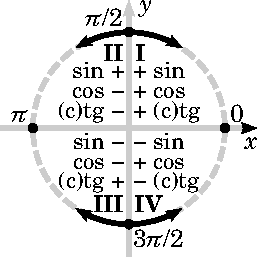
\includegraphics{drawing.pdf}\par}
\end{column*}

{\bold Следствие.} Для обратных функций верно:

\begin{tabularx}{\textwidth}{C@{\quad\quad}C}
$\begin{aligned}
\arcsin x+\arccos x&=\pi/2\\
\arctg x+\arcctg x&=\pi/2
\end{aligned}$ &
$\begin{aligned}
\arccos x+\arccos(-x)&=\pi\\
\arcctg x+\arcctg(-x)&=\pi
\end{aligned}$
\end{tabularx}

\subsection{Формулы понижения степени}

Из формул двойного угла и основного тригонометрического тождества следует:\par
% ---
\begin{tabularc}{0pt}{0pt}{c @{\quad\quad} c}{c}
$\begin{aligned}
\cos^2\frac{\alpha}{2}&=\frac{\cos\alpha+1}{2}\\
\sin\trsp^2\frac{\alpha}{2}&=\frac{1-\cos\alpha}{2}
\end{aligned}$ &
$\begin{aligned}
\tg\trsp^2\frac{\alpha}{2}&=\frac{1-\cos\alpha}{\cos\alpha+1}\\
\ctg\trsp^2\frac{\alpha}{2}&=\frac{1-\cos\alpha}{\cos\alpha+1}
\end{aligned}$
\end{tabularc}

Из них легко выводятся формулы {\ital половинного угла}.

\subsection{Сумма и разность двух функций}

Из формул суммы и разности двух углов следует:
% ---
\begin{align*}
\sin\alpha\pm\sin\beta&=2\sin\frac{\alpha\pm\beta}{2}\cos\frac{\alpha\mp\beta}{2}\\[-2pt]
\cos\alpha+\cos\beta&=2\cos\frac{\alpha+\beta}{2}\cos\frac{\alpha-\beta}{2}\\[-2pt]
\cos\alpha-\cos\beta&=-2\sin\frac{\alpha+\beta}{2}\sin\frac{\alpha-\beta}{2}\\
\end{align*}\\[-34pt]
% ---
$$a\sin\alpha+b\cos\alpha=c\sin(\alpha+\phi)=c\cos(\alpha-\phi),\ c=\sqrt{a^2+b^2}$$
% ---
Из них можно вывести формулы {\ital произведения двух функций}.

{\bold Доказательство.} Рассмотрим сумму синусов:
% ---
$$\sin(x+y)+\sin(x-y)=$$
$$\sin x\cos y+\sin y\cos x+\sin x\cos y-\sin y\cos x=2\sin x\cos y$$
% ---
Введём обозначения:
% ---
$$\begin{cases}
x+y=\alpha\\
x-y=\beta
\end{cases}\hspace*{-12pt}\iff
\begin{cases}
2x=\alpha+\beta\\
2y=\alpha-\beta
\end{cases}\hspace*{-12pt}\iff
\begin{cases}
x=\frac{\alpha+\beta}{2}\\
y=\frac{\alpha-\beta}{2}
\end{cases}$$
% ---
Таким образом,
% ---
$$\sin\alpha+\sin\beta=2\sin\frac{\alpha+\beta}{2}\cos\frac{\alpha-\beta}{2}.\qedw$$
% ---
Похожие формулы доказываются аналогично.$\qedw$\par

Рассмотрим синус суммы двух углов:
% ---
$$c\sin(\alpha+\phi)=c\sin\alpha\cos\phi+c\sin\phi\cos\alpha$$
% ---
Обозначим $a=c\cos\phi$, $b=c\sin\phi$ и найдём сумму квадратов:
% ---
$$a^2+b^2=c^2(\sin\trsp^2\phi+\cos^2\phi)=c^2\iff c=\sqrt{(a^2+b^2)}\qedw$$
% ---
Случай с косинусом доказывается аналогично.$\qedb$

\subsection{Подстановка Вейерштрасса}

Тригонометрические функции от $\alpha$ можно выразить через тангенс от $\alpha/2$
{\ital\color{desc}(К. Вейерштрасс)}:
% ---
$$\sin\alpha=\frac{2\tg\frac{\alpha}{2}}{1+\tg\trsp^2\frac{\alpha}{2}}\quad\quad
\cos\alpha=\frac{1-\tg\trsp^2\frac{\alpha}{2}}{1+\tg\trsp^2\frac{\alpha}{2}}$$
% ---
{\bold Доказательство.} Распишем каждую функцию:
% ---
$$\sin\alpha=\frac{2\sin\frac{\alpha}{2}\cos\frac{\alpha}{2}}{\sin\trsp^2\frac{\alpha}{2}
+\cos^2\frac{\alpha}{2}}=\frac{2\tg\frac{\alpha}{2}}{1+\tg\trsp^2\frac{\alpha}{2}}\qedw$$
$$\cos\alpha=\frac{\cos^2\frac{\alpha}{2}-\sin\trsp^2\frac{\alpha}{2}}{\sin\trsp^2\frac
{\alpha}{2}+\cos^2\frac{\alpha}{2}}=\frac{1-\tg\trsp^2\frac{\alpha}{2}}{1+\tg\trsp^2\frac
{\alpha}{2}}\qedb$$

\section{Теория множеств}

\subsection{Определение}

{\bold Множеством} называется объединение {\ital различных} объектов --- {\ital элементов} множества --- в единое целое.

\begin{theorem}
{\bold Способы задания множеств.}
% ---
\begin{list*}[][\#]
\item Перечислением {\ital (списком элементов)}
\item Порождающей процедурой
\item Разрешающей процедурой
\end{list*}
\end{theorem}

Множество $A$ есть {\bold подмножество} $B$, если все элементы $A$ являются элементами $B$:
% ---
$$A\subseteq B$$  
% ---
Множество $A$ есть {\bold надмножество} $B$, если все элементы $B$ являются элементами $A$:
% ---
$$A\supseteq B$$
% ---
Подмножество {\bold собственное} {\ital (строгое)}, если оно {\ital не равно} исходному множеству:
% ---
$$A\subseteq B\land A\neq B\implies A\subset B$$
% ---
\begin{theorem}
{\bold Булеан} множества ${\mathcal B}(A)$ --- множество всех его подмножеств:
% ---
$${\mathcal B}(A)=\{X\mid X\subseteq A\}$$
% ---
{\ital Мощность} булеана определяется формулой:
% ---
$$\abs{{\mathcal B}(A)}=2^{\abs{A}}$$
\end{theorem}
% ---
\begin{theorem}
{\bold Метод взаимного включения.} Множества $A$ и $B$ {\ital равны}, если они содержат одни и те же элементы:
% ---
$$A\subseteq B\land A\supseteq B$$
\end{theorem}

\begin{theorem}
{\bold Пустое множество} $\emptyset$ не содержит {\ital ни одного элемента} и есть подмножество любого множества.

{\bold Универсум} $\mathbb{U}$ --- широкое множество, которое состоит из всех элементов {\ital исследуемой области}.
\end{theorem}

{\bold Конечным} множество состоит из {\ital конечного} числа элементов, а {\bold бесконечное} множество --- из {\ital бесконечного}.

\begin{theorem}
{\ital Бесконечные} множества делятся на два вида:
% ---
\begin{list*}
\item {\bold cчётное}: равномощно множеству $\mathbb{N}$ {\ital\color{desc} (его можно пронумеровать)}
\item {\bold несчётное}: не равномощно $\mathbb{N}$ {\ital\color{desc} (его нельзя пронумеровать)}
\end{list*}
\end{theorem}

{\bold Мощность} {\ital конечного} множества --- число его элементов.

\subsection{Вектор}

{\bold Вектор} {\ital (кортеж, или упорядоченная n-ка)} --- упорядоченный набор элементов --- {\ital координат (компонент)} вектора.

{\bold Размерность} вектора --- число его координат.

\begin{theorem}
{\bold Декартово} {\ital (прямое)} {\bold произведение} множеств $X_1,\dots,X_n$ --- множество векторов вида:
% ---
$$X_1\times\dots\times X_n=\{(x_1,\dots,x_n)\mid x_1\in X_1,\dots,x_n\in X_n\}$$
% ---
Свойства:
% ---
\begin{list*}
\item дистрибутивность относительно {\ital пересечения} $\cap$
\item дистрибутивность относительно {\ital разности} $\backslash$
\item {\ital *не коммутативность}
\item {\ital *не ассоциативность}
\item $(A\cap B)\times(C\cap D)=(A\times C)\cap(B\times D)$
\end{list*}
\end{theorem}
% ---
{\bold Декартова степень} множества --- прямое произведение одинаковых множеств:
% ---
$$A^3=A\times A\times A$$
% ---
\begin{theorem}
{\bold Теорема.} Мощность декартова произведения конечных множеств равна {\ital произведению мощностей} данных множеств:
% ---
$$\abs{A_1\times\dots\times A_n}=\abs{A_1}\times\dots\times\abs{A_n}$$
\end{theorem}

\subsection{Отношение}

{\bold Отношение} $\rho$ между множествами $X_1,\dots,X_n$ --- подмножество их {\ital декартова произведения}.

\begin{theorem}
{\bold Бинарное} отношение включает {\ital два} множества, что можно упрощённо записать:
% ---
$$x\in X,\ y\in Y, \langle x, y\rangle\in\rho=:x\rho y$$
% ---
{\bold Унарное} отношение {\ital\color{desc} (свойство)} включает в себя...?
\end{theorem}

\begin{tabularc}{0pt}{0pt}{r @{ --- } l}{n}
$X\supseteq D_\rho$ & область определения {\bold (прообраз)} отношения\\
$Y\supseteq E_\rho$ & область значений {\bold (образ)} отношения.
\end{tabularc}
% ---
{\bold Наложение} {\ital (сюръекция)} --- бинарное отношение с $Y=E_\rho$:
% ---
$$\begin{gathered}
\forall y\in Y\ \exists x\in D_\rho\colon x\rho y\\
\rho\colon X\twoheadrightarrow Y
\end{gathered}$$
% ---
У {\bold частично определённого} бинарного отношения $X\neq D_\rho$:
% ---
$$\exists x\in X\ \forall y\in E_\rho\colon x\not\rho y$$

\subsection{Виды отношений}

{\bold Вложение} {\ital (инъекция, мономорфизм)} --- бинарное отношение $\rho$ вида:
% ---
$$\begin{gathered}
\forall x_1,x_2\in D_\rho\ \exists y\in E_\rho\colon x_1\rho y,\ x_2\rho y\iff x_1=x_2\\
\rho\colon X\hookrightarrow Y
\end{gathered}$$
% ---
{\bold Функция} {\ital (отображение)} --- бинарное отношение $\rho$ вида:
% ---
$$\begin{gathered}
\forall x\in D_\rho\ \exists!y\in E_\rho\colon x\rho y\\
\rho\colon X\xrightarrow{x\mapsto y} Y
\end{gathered}$$
% ---
{\bold Изоморфизм} {\ital (биекция)} --- бинарное отношение, которое является {\ital и вложением, и наложением}:
% ---
$$\rho\colon X\xrightarrow{\sim}Y$$
% ---
\begin{theorem}
{\bold Композиция} {\ital (суперпозиция)} бинарных отношений\\ $f\subseteq X\times Y,\ g\subseteq Y\times Z$ --- такое $h\subseteq X\times Z\iff f\circ g$, что:
% ---
$$\forall x\in X,\ z\in Z\exists y\in Y\ x(f\circ g)z\iff xfy\land ygz$$
% ---
Свойства:

\begin{list*}
\item ассоциативность
\item {\ital *не коммутативность}
\end{list*}
\end{theorem}

\begin{theorem}
{\bold Обратное} бинарное отношение $\rho^{-1}$ получается переста"=новкой исходных множеств в декартовом произведении:
% ---
$$\rho\subseteq X\times Y\iff\rho^{-1}\subseteq Y\times X$$
% ---
Свойства:
% ---
\begin{list*}
\item инволютивность
\item дистрибутивность относительно {\ital пересечения} $\cap$
\item дистрибутивность относительно {\ital объединения} $\cup$
\item дистрибутивность относительно {\ital композиции} $\circ$:
% ---
$$(P\circ Q)^{-1}=Q^{-1}\circ R^{-1}$$
\end{list*}
\end{theorem}

\subsection{Свойства отношений}

Пусть $\ast\subseteq X^2$ --- произвольное бинарное отношение.

Отношение $\ast$ {\ital симметрично}, когда
% ---
$$\forall x,y\in X\ x\ast y=y\ast x.$$
% ---
Отношение $\ast$ {\ital антисимметрично}, когда
% ---
$$\forall x,y\in X\ x\ast y\land y\ast x\implies x=y$$
% ---
Отношение $\ast$ {\ital транзитивно}, когда
% ---
$$\forall x,y,z\in X\ x\ast y\land y\ast z\implies x\ast z$$
% ---
Отношение $\ast$ {\ital рефлексивно}, когда
% ---
$$\forall x\in X\ x\ast x$$
% ---
Отношение $\ast$ {\ital антирефликсивно}, когда
% ---
$$\forall x\in X\ \lnot (x\ast x)$$

\subsection{Эквиваленция}

{\bold Эквиваленция} --- бинарное отношение...

\subsection{Ограничение и продолжение}

{\ital Ограничением} отображения $f\colon X\to Y$ на $S\subseteq D_f$ называется
такое $f\vert_S\colon S\to Y$, что
% ---
$$\forall s\in S\colon f\vert_S(s)=f(s).$$
% ---
В свою очередь, $f$ является {\ital продолжением} отображения $f\vert_S$.

\subsection{Промежутки числовой прямой}

{\bold Отрезок} --- множество вида:
% ---
$$[a,b]=\{x\in\mathbb{R}\mid a\leq x\leq b\}$$
% ---
{\bold Интервал} --- множество вида:
% ---
$$[a,b]=\{x\in\mathbb{R}\mid a\less x\less b\}$$
% ---
{\bold Полуинтервал} --- множества вида:
% ---
$$\begin{gathered}
[a,b)=\{x\in\mathbb{R}\mid a\leq x\less b\}\\
(a,b]=\{x\in\mathbb{R}\mid a\less x\leq b\}
\end{gathered}$$
% ---
{\bold Луч} --- множества вида:
% ---
$$\begin{gathered}
[a,+\infty)=\{x\in\mathbb{R}\mid x\geq a\}\\
(a,+\infty)=\{x\in\mathbb{R}\mid x\greater a\}\\
(-\infty,b]=\{x\in\mathbb{R}\mid x\leq a\}\\
(-\infty,b)=\{x\in\mathbb{R}\mid x\less a\}
\end{gathered}$$
% ---
\begin{theorem}
{\bold $\symbf{\varepsilon}$-окрестность} точки $x_0\in\mathbb{R}$ --- интервал вида:
% ---
$$U_\varepsilon(x_0)=\{x\in\mathbb{R}\colon\abs{x-x_0}\less\varepsilon\}=(x_0-\varepsilon,x_0+\varepsilon)$$

Особые случаи:
% ---
$$\begin{gathered}
U_\varepsilon(+\infty)=(1/\varepsilon,+\infty)\\
U_\varepsilon(-\infty)=(-\infty,-1/\varepsilon)
\end{gathered}$$
\end{theorem}
% ---
{\bold Проколотая} $\varepsilon$-окрестность точки $x_0$ не включает саму точку:\\[-8pt]
% ---
$$\overset{\circ}{U}_\varepsilon(x_0)=U_\varepsilon(x_0)\backslash\{x_0\}$$
% ---
{\bold Правосторонняя (левосторонняя)} $\varepsilon$-окрестность точки $x_0$
не содержит свою {\ital левую  (правую)} половину:
% ---
$$U_{\varepsilon+}(x_0)=[x_0;\varepsilon)\quad\quad U_{\varepsilon-}(x_0)=(\varepsilon;x_0]$$

\subsection{Ограниченное множество}

Множество $M$ {\bold ограничено сверху}, если:
% ---
$$\forall m\in M\ \exists C\in\mathbb{R}\colon m\leq C$$
% ---
{\bold Верхняя граница} множества $M$ --- такое $N\in\mathbb{R}$, что:
% ---
$$\forall x\in M\colon x\leq N$$
% ---
{\bold Наибольший элемент} {\ital (максимум)} множества $M$ --- такое $\max M\in M$, что:
% ---
$$\forall x\in M\ x\leq\max M$$
% ---
{\bold Супремум} {\ital (точная верхняя граница)} --- такая верхняя граница множества $M$ --- $\sup M$, что:
% ---
$$\forall\varepsilon\greater 0\ \exists m\in M\colon m\in U_{\varepsilon-}(\sup M)$$
% ---
\begin{theorem}
{\bold Связь супремума с максимумом.} Если у множества $M$ существует $\max M$, то:
% ---
$$\sup M=\max M$$ 
\end{theorem}
% ---
\begin{theorem}
{\bold Принцип точной грани.} Если непустое множество $M$ ограничено сверху, то существует {\ital единственный} $\sup M$.
\end{theorem}
% ---
Множество $M$ {\bold ограничено снизу}, если:
% ---
$$\forall m\in M\ \exists C\in\mathbb{R}\colon m\geq C$$
% ---
{\bold Нижняя граница} множества $M$ --- такое $N\in\mathbb{R}$, что:
% ---
$$\forall x\in M\colon x\geq N$$
% ---
{\bold Наименьший элемент} {\ital (минимум)} множества $M$ --- такое $\min N\in M$, что:
% ---
$$\forall x\in M\ x\geq\min M$$
% ---
{\bold Инфимум} {\ital (точная нижняя граница)} --- такая нижняя граница множества $M$ --- $\inf M$, что:
% ---
$$\forall\varepsilon\greater 0\ \exists m\in M\colon m\in U_{\varepsilon+}(\inf M)$$
% ---
\begin{theorem}
{\bold Связь инфимума с минимумом.} Если у множества $M$ существует $\min M$, то:
% ---
$$\inf M=\min M$$ 
\end{theorem}
% ---
\begin{theorem}
{\bold Принцип точной грани.} Если непустое множество $M$ ограничено снизу, то существует {\ital единственный} $\inf M$.
\end{theorem}
% ---
{\bold Ограниченное} множество $M$ ограничено {\ital и сверху, и снизу}:
% ---
$$\exists N\in\mathbb{R}\colon\forall x\in M\ \abs{x}\leq N$$
% ---
\begin{theorem}
{\bold Принцип Архимеда.} Пусть $x\in\mathbb{R}^+$. Тогда справедливо:
% ---
$$\forall y\in\mathbb{R}\ \exists!k\in\mathbb{Z}\colon (k-1)x\less y\leq kx$$
% ---
{\bold Следствие.} Для $x\in\mathbb{R}$ существует такое $k\in\mathbb{Z}$, что:
% ---
$$k\leq x\less k+1\qquad{\color{desc} (k=[x])}$$
\end{theorem}

\subsection{Принцип Кантора}

Последовательность вложенных отрезков содержит точки $\xi$, которые принадлежат им всем:
% ---
$$\forall n\in\mathbb{N}\ \exists\xi\in[a_n;b_n]\subset[a_{n-1};b_{n-1}]$$
% ---
Если $n\to\infty$, $(b_n-a_n)\to 0$, то $\xi$ единственна:
% ---
$$\lim_{n\to\infty}a_n=\sup\{a_n\}=\lim_{n\to\infty}b_n=\inf\{b_n\}=\xi$$
% ---
{\bold Доказательство.} По теореме Вейерштрасса:
% ---
$$\lim_{n\to\infty}a_n=\sup\{a_n\}\quad\quad\lim_{n\to\infty}b_n=\inf\{b_n\}$$
% ---
Значит, $\forall(n\in\mathbb{N},\ \xi\in[\sup\{a_n\};\inf\{b_n\}])\ \xi\in[a_n;b_n]$.
$\qedw$

Если $\inf\{b_n\}=\sup\{a_n\}$, то $\xi$ единственна:
% ---
$$0=\inf\{b_n\}-\sup\{a_n\}=\lim_{n\to\infty}b_n-\lim_{n\to\infty}a_n=\lim_{n\to\infty}
(b_n-a_n)\qedb$$

\section{Алгебра логики}

\subsection{Определение}

{\bold Алгебра логики} --- алгебраическая структура, которая образована двухэлементным множеством $\{0;1\}$.

{\bold Высказывание} --- повествовательное предложение, о кото"=ром можно сказать в данный момент, что оно {\ital истинно} или {\ital ложно}.

{\bold Логическая связка} --- операция алгебры логики:
% ---
\begin{list*}[][\#]
\item{\ital Инверсия} «$\lnot$» --- логическое {\ital «не»}.
\item{\ital Конъюнкция} «$\land$» --- логическое {\ital «и»}.
\item{\ital Дизъюнкция} «$\lor$» --- логическое {\ital «или»}.
\item{\ital Строгая дизъюнкция} «$\dot{\lor}$» --- логическое {\ital «искл. или»}.
\item{\ital Импликация} «$\rightarrow$» --- логическое {\ital «$\implies$»}.
\item{\ital Эквиваленция} «$\equiv$» --- логическое {\ital «$\iff$»}.
\end{list*}

\subsection{Свойства}

Конъюнкция и дизъюнкция {\ital коммутативны}, {\ital ассоциативны} и {\ital дистрибутивны} относительно друг друга.
% ---
\begin{theorem}
{\bold Идемпотентность.}
% ---
$$A\land A=A\qquad A\lor A=A$$
\end{theorem}
% ---
\begin{theorem}
{\bold Закон противоречия} и {\bold исключённого третьего.}
% ---
$$A\land\overline{A}=0\qquad A\lor\overline{A}=1$$
\end{theorem}
% ---
\begin{theorem}
{\bold Закон поглощения.}
% ---
$$\begin{gathered}\begin{aligned}
&A\land 1=A &\quad &A\land 0=0\\
&A\lor 1=1 &\quad &A\lor 0=A
\end{aligned}\\
A\land (A\lor B)=A\qquad A\lor (A\land B)=A\\
A\land (\overline{A}\lor B)=A\land B\qquad A\lor (\overline{A}\land B)=A\lor B\end{gathered}$$
\end{theorem}
% ---
\begin{theorem}
{\bold Закон де Мóргана.}
% ---
$$\overline{A\land B}=\overline{A}\lor\overline{B}\qquad\overline{A\lor B}=\overline{A}\land\overline{B}$$
\end{theorem}
% ---
\begin{theorem}
{\bold Закон склеивания.}
% ---
$$\begin{aligned}
&(A\lor B)\land(A\lor \overline{B})=A\\
&(A\land B)\lor(A\land \overline{B})=A\\
\end{aligned}$$
\end{theorem}

\subsection{Нормальная форма}

{\bold Терм} --- компонент логической функции:

\begin{list*}
\item{\bold макстерм} --- переменные прямой и инверсной форм связаны {\ital дизъюнкцией}
\item{\bold минтерм} --- переменные прямой и инверсной форм связаны {\ital конъюнкцией}
\end{list*}
% ---
{\bold Ранг} {\ital терма} --- число переменных, которые в него входят.

{\bold Нормальная дизъюнктивная форма} {\ital (DNF)} --- дизъюнк"=ция минтермов любого ранга.

{\bold Нормальная конъюнктивная форма} {\ital (CNF)} --- конъюнк"=ция макстермов любого ранга:
% ---
\begin{theorem}
\begin{tabularcx}{0pt}{0pt}{C@{\hspace*{-16pt}}C}{\textwidth}
$\begin{aligned}
A\dot{\lor}B&=(A\lor B)\land(\overline{A}\lor\overline{B})\\
A\equiv B&=(\overline{A}\lor B)\land(A\lor\overline{B})
\end{aligned}$\hspace*{-18pt} & $A\rightarrow B=\overline{A}\lor B$
\end{tabularcx}
\end{theorem}
% ---
{\bold Нормальная импликативная форма} {\ital (INF)} --- конъюнк"=ция макстермов любого ранга, которые заменены имплика"=цией:
% ---
$$A\lor B=(\overline{A}\rightarrow B)\land(\overline{B}\to A)$$

\section{Общая алгебра}

\subsection{Алгебраическая операция}

$n$-местная {\bold алгебраическая операция} $\ast$ --- отображение:
% ---
$$\ast\colon X_1\times\dots\times X_n\to Y$$
% ---
Операция $\ast$ {\bold внутренняя} для множества $X$ {\ital (множество $X$ {\boldital замкнуто} относительно операции $\ast$)}, если:
% ---
$$X_i\subseteq X\land Y\subseteq X$$
% ---
Иначе операция $\ast$ {\bold внешняя} для множества $X$ {\ital (множество $X$ {\boldital не замкнуто} относительно операции $\ast$)}.

{\bold Нейтральным} от-но $\ast$ наз-ся такой элемент $e\in X$, что:
% ---
$$\forall x\in X\ e\ast x=x\ast e=x$$
% ---
\begin{theorem}
Если нейтральный элемент $e$ от-но $\ast$ существует, то он {\ital единственный}.
\end{theorem}
% ---
{\bold Поглощающим} от-но $\ast$ наз-ся такой элемент $w\in X$, что:
% ---
$$\forall x\in X\ w\ast x=x\ast w=w$$
% ---
\begin{theorem}
Если поглощающий элемент $w$ от-но $\ast$ существует, то он {\ital единственный}.
\end{theorem}
% ---
{\bold Симметричным} {\ital (противоположным, обратным)} к~элементу $x\in X$ от-но $\ast$ наз-ся такой элемент $x^{-1}\in X$, что:
% ---
$$x\ast x^{-1}=x^{-1}\ast x=e\text{ {\ital\color{desc}(нейтр.)}}$$
% ---
\begin{theorem}
Если симметричный элемент $x^{-1}$ к элементу $x$ от-но ассоциативной $\ast$ существует, то он {\ital единственный}.
\end{theorem}
% ---
\begin{theorem}
{\bold Теорема.} Если $y\colon X\to Y$ и $x\colon Y\to X$ --- отображения, то $y$ 
{\ital инъективно}, а $x$ {\ital сюръективно}.
\end{theorem}

{\bold Доказательство.} По условию, множество $X$ накладывается на себя.
Значит, $f$ {\ital всюду определено}.\par

Так как $g$ функционально, то
% ---
$$\forall x_1,x_2\in X\ \exists y\in E_f\colon x_1fy,\ x_2fy\iff x_1=x_2,$$
% ---
то есть $f$ {\ital инъективно}.$\qedw$\par

Когда $X$ накладывается на себя, то
% ---
$$\forall x\in E_g\ \exists y\in D_g\colon x\mapsto y,$$
% ---
то есть $g$ {\ital сюръективно}.$\qedb$

\subsection{Свойства операций}

Пусть $\ast\colon X^2\to X$, $\circ\colon X^2\to X$ --- алгебраические операции.

Операция $\ast$ {\bold коммутативна}, когда
% ---
$$\forall x,y\in X\ x\ast y=y\ast x$$
% ---
Операция $\ast$ {\bold ассоциативна}, когда
% ---
$$\forall x,y,z\in X\ (x\ast y)\ast z=x\ast(y\ast z)$$
% ---
Операция $\ast$ {\bold дистрибутивна} относительно $\circ$, когда
% ---
$$\forall x,y,z\in X\ 
\begin{cases*}
&x\ast(y\circ z)=(x\ast y)\circ (x\ast z)\text{ {\ital\color{desc} (дистр. справа)}}\\
&(x\circ y)\ast z=(x\ast z)\circ(y\ast z)\text{ {\ital\color{desc} (дистр. слева)}}
\end{cases*}$$
% ---
\begin{theorem}
{\bold Теорема.} Пусть $e$ --- нейтральный элемент от-но операции $\ast$, дистрибутивной от-но операции $\circ$. Тогда $e$ --- {\ital поглощающий элемент} от-но $\circ$.
\end{theorem}

{\ital (Работает ли теорема выше в обратную сторону?)}

\subsection{Алгебраическая структура}

{\bold Алгебраическая структура} {\ital (система)} --- множество $X$ с~введёнными на нём 
алгебраическими операциями:
% ---
$$(X,\ast_1,\dots,\ast_n)$$
% ---
Для {\bold голоморфных} структур $(M,\circ)$, $(N,\ast)$ существует отображение $f$ вида:
% ---
$$f\colon M\to N\iff\forall x,y\in M\ f(x\circ y)=f(x)\ast f(y)$$
% ---
Для {\bold изоморфных} структур $(M,\circ)$, $(N,\ast)$ существует изоморфизм $f$ вида:
% ---
$$\begin{gathered}
f\colon M\xrightarrow{\sim} N\iff\forall x,y\in M\ f(x\circ y)=f(x)\ast f(y)\\
(M,\circ)\simeq (N,\ast)
\end{gathered}$$

\subsection{Виды структур}

{\bold Магма} {\ital (группоид)} --- алгебраическая структура $(X,\ast)$ с~внутренней бинарной операцией $\ast$.

{\bold Группа} --- магма, для которой справедливо:
% ---
\begin{list*}[][\#]
\item Ассоциативность $\ast$ --- для {\bold полугруппы}.
\item $\exists$ нейтральный элемент от-но $\ast$ --- для {\bold моноида}.
\item $\forall x\in G\ \exists$ симметричный элемент от-но $\ast$.
{\color{desc}\item Коммутативность $\ast$ --- для {\bold абелевой} группы.}
\end{list*}
% ---
{\bold Кольцо} --- такая алгебраическая структура $(X,+,\cdot)$, что:
% ---
\begin{list*}[][\#]
\item Абелева группа относительно {\ital сложения} $+$.
\item Дистрибутивность {\ital умножения} относительно {\ital сложения}.
{\color{desc}\item Ассоциативность {\ital умножения} $\cdot$ --- для {\bold ассоциативного кольца}.}
{\color{desc}\item Коммутативность {\ital умножения} --- для {\bold коммутативного кольца}.}
{\color{desc}\item $\exists$ нейтральный элемент от-но $\cdot$ --- для {\bold кольца с~единицей}.}
{\color{desc}\item Группа относительно {\ital умножения} --- для {\bold поля}.}
\end{list*}
% ---


{\bold Подгруппа} --- подмножество $H$ аддитивной абелевой группы $G$, которое замкнуто по сложению на всей группе $G$:
% ---
$$+\colon H\times G\to H$$
% ---
{\bold Идеал} --- подмножество $I$ кольца $A$, которое замкнуто по умножению на всём кольце $A$:
% ---
$$\cdot\colon I\times A\to I$$

\subsection{Числовые системы}

{\bold Система натуральных чисел} --- коммутативная аддитивная и мультипликативная полугруппа $\langle\mathbb{N};\ +,\times\rangle$.\par

{\bold Система целых чисел} --- коммутативное кольцо $\langle\mathbb{Z};\ +,\times\rangle$.
\par

{\bold Система рациональных чисел} --- упорядоченное поле $\langle\mathbb{Q};\ +,\times
\rangle$.\par

{\bold Система действительных чисел} --- непрерывное упорядо"=ченное поле $\langle\mathbb
{R};\ +,\times\rangle$.

\subsection{Действительные числа}

{\bold Система действительных чисел} --- алгебраическая структура $\langle\mathbb{R};\ +,\cdot,\leq\rangle$, в которой выполняется следующая {\ital аксиоматика}.
% ---
\begin{theorem}
{\bold Аксиомы сложения.} {\ital Сложение} --- алгебраическая операция $+\colon\mathbb{R}^2\to\mathbb{R}$.

Свойства:
% ---
\begin{list*}[][\#]
\item коммутативность
\item ассоциативность
\item существование нейтрального элемента
\item существование противоположного {\ital (симметричного)} элемента
\end{list*}
% ---
Следствия из аксиом:
% ---
\begin{list*}[][\#]
\item Единственность нуля {\ital (нейтрального элемента)}.
\item Единственность противоположного {\ital (симметричного)} элемента.
\item Умножение на $-1$ порождает противоположный элемент.
\end{list*}
\end{theorem}

\begin{theorem}
{\bold Аксиомы умножения.} {\ital Умножение} --- алгебраическая операция $\cdot\colon\mathbb{R}^2\to\mathbb{R}$.

Свойства:
% ---
\begin{list*}[][\#]
\item коммутативность
\item ассоциативность
\item существование нейтрального элемента
\item существование обратного {\ital (симметричного)} элемента
\end{list*}
% ---
Следствия из аксиом:
% ---
\begin{list*}[][\#]
\item Единственность единицы {\ital (нейтрального элемента)}.
\item Единственность обратного {\ital (симметричного)} элемента.
\item Нуль --- поглощающий элемент.
\end{list*}
\end{theorem}

\begin{theorem}
{\bold Связь сложения и умножения.} {\ital\color{desc} (Дистрибутивность $\cdot$ от-но $+$)}
% ---
$$\forall x,y,z\in\mathbb{R}\ x\cdot(y+z)=x\cdot y+x\cdot z$$
\end{theorem}

\begin{theorem}
{\bold Аксиомы порядка.} {\ital Неравенство} --- алгебраическая операция $\leq\colon\mathbb{R}^2\to\mathbb{R}$.

Свойства:
% ---
\begin{list*}[][\#]
\item рефлексивность
\item антисимметричность
\item транзитивность
\item {\ital линейная упорядоченность:}
% ---
$$\forall x,y\in\mathbb{R}\ (x\leq y)\lor(y\leq x)$$
\end{list*}
\end{theorem}

\begin{theorem}
{\bold Связь сложения и порядка.}
% ---
$$\forall x,y,z\in\mathbb{R}\ x\leq y\iff x+z\leq y+z$$
% ---
{\bold Следствие.}
% ---
$$(x\leq y)\land(z\leq k)\implies x+z\leq y+k$$
\end{theorem}

\begin{theorem}
{\bold Связь умножения и порядка.}
% ---
$$\forall x,y,z\in\mathbb{R}\ (0\leq x)\land(0\leq y)\implies 0\leq x\cdot y$$
% ---
{\bold Следствия.}
% ---
$$\begin{aligned}
0\greater x\land 0\greater y&\implies 0\less xy\\
0\greater x\land 0\less y&\implies 0\greater xy\\
x\less y\land z\greater 0&\implies xz\less yz\\
x\less y\land z\less 0&\implies xz\greater yz
\end{aligned}$$
\end{theorem}

\begin{theorem}
{\bold Аксиома полноты.} Пусть $X,Y\subset\mathbb{R}$ и $X\neq\emptyset$, $Y\neq\emptyset$. 
% ---
$$(\forall x\in X,\ y\in Y\ x\leq y)\implies\exists c\in\mathbb{R}\ x\leq c\leq y$$
\end{theorem}

\begin{theorem}
{\bold Лемма.} {\ital\color{desc}(Сравнение нуля и единицы)}
% ---
$$0\less 1$$
\end{theorem}

Доказательство леммы следует из {\ital аксиом порядка}.

\subsection{Подмножества $\mathbb{R}$}

Для {\bold индуктивного} множества $X\subset\mathbb{R}$ справедливо:
% ---
$$\forall x\in X\ (x+1)\in X$$
% ---
Примеры индуктивных множеств: $\mathbb{N}$, $\mathbb{Z}$, $\mathbb{Q}$, $\mathbb{I}$, $\mathbb{R}$.

\begin{theorem}
{\bold Принцип математической индукции.} Пусть $X\subset\mathbb{N}$:
% ---
$$(\underbrace{1\in X}_{1}\land\underbrace{\forall x\in X\ (x+1)\in X}_{2})\implies X=\mathbb{N}$$
% ---
\begin{list*}[][\#]
\item Базис индукции.
\item Индукционный шаг.
\end{list*}
\end{theorem}
% ---
{\bold Целые числа} $\mathbb{Z}$ --- объединение $\mathbb{N}$ с множеством чисел, противоположных к $\mathbb{N}$, и нулём.

{\bold Рациональные числа} $\mathbb{Q}$ --- множество чисел вида:
% ---
$$m\cdot n^{-1},\quad m,n\in\mathbb{Q}$$
% ---
{\bold Иррациональные числа} $\mathbb{I}$ --- множество вида:
% ---
$$\mathbb{I}=\mathbb{R}\backslash\mathbb{Q}$$

\subsection{Расширенная числовая прямая}

{\bold Расширенная числовая прямая} --- расширение множества действительных 
чисел:
% ---
$$\bar{\mathbb{R}}=\mathbb{R}\cup\{\pm\infty\}$$
% ---
Свойства бесконечности:
% ---
$$\begin{gathered}
(\pm\infty)+(\pm\infty)=\pm\infty\\
(\pm\infty)\cdot(\pm\infty)=+\infty\\
(+\infty)\cdot(-\infty)=-\infty\\
x+(\pm\infty)=(\pm\infty)+x=\pm\infty,\quad x\in\mathbb{R}\\
x\cdot(\pm\infty)=(\pm\infty)\cdot x=\begin{cases*}
&\pm\infty,\quad x\greater 0\\
&\mp\infty,\quad x\less 0
\end{cases*}\\
\frac{x}{0}=\begin{cases*}
&+\infty,\quad x\greater 0\\
&-\infty,\quad x\less 0
\end{cases*}\\
\frac{x}{\infty}=0,\quad x\in\mathbb{R}
\end{gathered}$$

\newpage
\subsection{Комплексные числа}

{\bold Система комплéксных чисел} --- непрерывное поле:
% ---
$$\langle\mathbb{C}=\mathbb{R}^2;\ +,\cdot\rangle$$
% ---
{\bold Комплексное число} --- элемент $z=(a,b)\in\mathbb{C}$.
% ---
\begin{theorem}
{\bold Свойство.} Множество $\mathbb{C}$ включает в себя множество $\mathbb{R}$:
% ---
$$\forall a\in\mathbb{R}\ (a,0)\leftrightarrow a\implies\mathbb{R}\subset\mathbb{C}$$
\end{theorem}
% ---
{\bold Мнимая единица} --- комплексное число вида:
% ---
$$(0,1)\leftrightarrow i,\quad i^2=-1$$
% ---
{\bold Плоскость комплексных чисел} --- декартова система координат $Oab$ с биекцией вида:
% ---
$$z=(a,b)\leftrightarrow M(a,b)$$

\begin{list*}
\item $Oa$ есть действительная ось {\ital\color{desc}($a=\ren{z}$)}
\item $Ob$ есть мнимая ось {\ital\color{desc}($b=\imn{z}$)}
\end{list*}
% ---
\begin{theorem}
{\bold Свойство.} Комплексные числа {\ital равны}, если соответственно равны их действительные и мнимые части:
% ---
$$(a_1,b_1)=(a_2,b_2)\iff a_1=a_2\land b_1=b_2$$
\end{theorem}
% ---
\begin{theorem}
{\bold Формы записи.} Пусть $z=(a,b)\in\mathbb{C}$.
% ---
\begin{list*}
\item алгебраическая форма: $z=a+bi$
\item тригонометрическая форма: $z=\abs{z}(\cos\varphi+i\sin\varphi)$
\end{list*}
\end{theorem}

\subsection{Операции комплексных чисел}

\begin{theorem}
{\bold Сложение и умножение.} Пусть $z_1=(a,b)$, $z_2=(c,d)$:
% ---
$$\begin{aligned}
&z_1+z_2=(a,b)+(c,d)=(a+c,b+d)\\
&z_1\cdot z_2=(a,b)\cdot(c,d)=(ac-bd,ad+bd)
\end{aligned}$$
% ---
Cвойства операций {\ital индуцируются} из множества дейст"=вительных чисел $\mathbb{R}$. 
\end{theorem}

\begin{theorem}
{\bold Сопряжение} --- операция смены знака $\imn{z}$:
% ---
$$z=(a,b)\to\bar{z}=(a,-b)$$
% ---
Свойства:
% ---
\begin{list*}
\item дистрибутивность относительно {\ital сложения} $+$
\item дистрибутивность относительно {\ital умножения} $\cdot$
\end{list*}
\end{theorem}
% ---
\begin{theorem}
{\bold Модуль} комплексного числа $z$ --- расстояние $\rho(O;M)$:
% ---
$$\abs{z}=r=\abs{OM}=\sqrt{a^2+b^2}=\sqrt{z\bar{z}}$$
% ---
Свойства:
% ---
\begin{list*}
\item дистрибутивность относительно {\ital умножения} $\cdot$ {\ital (деления $\colon$)}
\end{list*}
\end{theorem}
% ---
\begin{theorem}
{\bold Аргумент} комплексного числа --- угол, образованный $\overrightarrow{OM}$ с~действительной осью:
% ---
$$\arg z=\varphi=\arctg\frac{b}{a},\quad\varphi\in(-\pi;\pi]$$
% ---
Свойства:
% ---
\begin{list*}
\item $\arg(z_1\cdot z_2)=\arg z_1+\arg z_2$
\item $\arg(z_1\slash z_2)=\arg z_1-\arg z_2$
\item $\arg z^n=n\arg z,\ n\in\mathbb{Z}$
\end{list*}
\end{theorem}
% ---
\begin{theorem}
{\bold Формула Муавра.} Возведение в степень числа $z\in\mathbb{C}$:
% ---
$$z^n=\abs{z}^n(\cos n\varphi+i\sin n\varphi),\quad n\in\mathbb{Z}$$
% ---
{\bold Следствие.} Корень $n$-й степени из числа $z\in\mathbb{C}$:
% ---
$$\sqrt[n]{z}=\sqrt[n]{\abs{z}}\left(\cos\frac{\varphi+2\pi k}{n}+i\sin\frac{\varphi+2\pi k}{n}\right),\quad k\in\mathbb{Z}$$
\end{theorem}
% ---
\begin{theorem}
{\bold Квадратный корень.} Корень из числа $z\in\mathbb{C}$:
% ---
$$\sqrt{z}=\pm\left(\sqrt{\frac{\abs{z}+a}{2}}+\sgnb{b}i\sqrt{\frac{\abs{z}-a}{2}}\right)$$
\end{theorem}

\subsection{Метрическое пространство}

{\ital Метрическое пространство} --- алгебраическая структура $\langle M;\ d\rangle$,
где $d$ --- метрика.\par

Метрика $d$ множества $M$ --- функция $d\colon M\times M\to R^+_0$, которая
определяет {\ital расстояние} между его двумя элементами.\par

Например, {\ital евклидова метрика} использует теорему Пифагора в $n$-мерном
пространстве:
% ---
$$d(x,y)=\sqrt{\sum^{n}_{k=1}(x_k-y_k)^2}$$
% ---
Для метрического пространства $\langle M;\ d\rangle,\ x,y,z\in M$ выполня"=ются
следующие {\ital аксиомы}:\par

--- $d(x,y)=0\iff x=y$ --- {\ital тождество};\\
--- $d(x,y)=d(y,x)$ --- {\ital симметрия};\\
--- $d(x,y)\leq d(x,z) + d(y,z)$ --- {\ital «неравенство треугольника»}.

\subsection{Длина отрезка}

{\bold Расстояние} между точками $A\langle a\rangle$ и $B\langle b\rangle$ ---
% ---
$$\abs{\overrightarrow{AB}}=\abs{a-b}\implies AB^2=(a-b)(\bar{a}-\bar{b})$$
% ---
{\ital Уравнение окружности} с центром $A\langle a\rangle$ радиуса $r$ ---
% ---
$$(z-a)(\bar{z}-\bar{a})=r^2$$

\subsection{Скалярное произведение векторов}

{\ital Скалярное произведение радиус-векторов} ---
% ---
$$2\overrightarrow{OA}\cdot\overrightarrow{OB}=a\bar{b}+\bar{a}b$$
% ---
{\bold Доказательство.} Пусть $A\langle a\rangle$, $B=\langle b\rangle$, $a=x_1+y_1i$, $b=x_2+y_2i$. Тогда:
% ---
$$a\bar{b}+\bar{a}b=(x_1+y_1i)(x_2-y_2i)+(x_1-y_1i)(x_2+y_2i)=$$
$$2(x_1x_2+y_1y_2)=2\overrightarrow{OA}\cdot\overrightarrow{OB}\qedb$$

Пусть $A\langle a\rangle$, $B\langle b\rangle$, $C\langle c\rangle$, $D\langle d\rangle$ --- четыре различные точки. Тогда {\ital скалярное произведение произвольных векторов} ---
% ---
$$2\overrightarrow{AB}\cdot\overrightarrow{CD}=(b-a)(\bar{d}-\bar{c})+(\bar{b}-\bar{a})(d-c)$$
% ---
{\bold Доказательство.} По условию:
% ---
$$2\overrightarrow{AB}\cdot\overrightarrow{CD}=2(\overrightarrow{OB}-\overrightarrow{OA})(\overrightarrow{OD}-\overrightarrow{OC})=$$
$$2(\overrightarrow{OB}\cdot\overrightarrow{OD}-\overrightarrow{OB}\cdot\overrightarrow{OC}-\overrightarrow{OA}\cdot\overrightarrow{OD}+\overrightarrow{OA}\cdot\overrightarrow{OC})=$$
$$\cancel{2}\cdot\frac{1}{\cancel{2}}(b\bar{d}+\bar{b}d-b\bar{c}-\bar{b}c-a\bar{d}-\bar{a}d+a\bar{c}+\bar{a}c)=$$
$$(a-b)(\bar{c}-\bar{d})+(\bar{a}-\bar{b})(c-d)\qedb$$

\subsection{Коллинеарность}

{\bold Коллинеарными} называются:
% ---
\begin{tabularcx}{3pt}{3pt}{@{--- } L}{\textwidth}
{\ital точки}, которые лежат на одной прямой;\\
{\ital векторы}, которые лежат на одной прямой или на~параллельных прямых.
\end{tabularcx}
% ---
\begin{theorem}
{\ital Критерий коллинеарности} точек $A$, $B$ с $O$:
% ---
$$\frac{a}{b}=\overline{\left(\frac{a}{b}\right)}\quad\text{или}\quad
\begin{sqcases*}
&a=0\\
&b=0
\end{sqcases*}$$
\end{theorem}
% ---
{\bold Доказательство.} Очевидно, что:
% ---
$$\left[\begin{aligned}
&\arg a-\arg b=0\\
&\arg a-\arg b=\pm\pi
\end{aligned}\right.\implies
\arg\frac{a}{b}=0;\pm\pi$$
% ---
По определению аргумента комплексного числа:
% ---
$$\frac{a}{b}\text{ --- действительное число}\implies\frac{a}{b}=\overline{\left(\frac{a}{b}\right)}\qedb$$
% ---
\begin{theorem}
{\ital Критерий коллинеарности} векторов $\overrightarrow{AB}$, $\overrightarrow{CD}$:
% ---
$$\frac{b-a}{d-c}=\overline{\left(\frac{b-a}{d-c}\right)}\quad\text{или}\quad
\left[\begin{aligned}
\overrightarrow{AB}=\overrightarrow{0}\\
\overrightarrow{CD}=\overrightarrow{0}\\
\end{aligned}\right.$$
\end{theorem}
% ---
{\bold Доказательство.} По определению комплексных чисел:
% ---
$$\overrightarrow{AB}\sim b-a,\ \overrightarrow{CD}\sim d-c$$
% ---
По критерию коллинеарности двух точек с $O$:
% ---
$$\frac{b-a}{d-c}=\overline{\left(\frac{b-a}{d-c}\right)}\qedb$$
% ---
Если $A$, $B$, $C$, $D$ лежат на одной окружности, то:
% ---
$$\overrightarrow{AB}\parallel\overrightarrow{CD}\iff\frac{b}{d}=\frac{a}{c}$$
% ---
\begin{theorem}
{\ital Критерий коллинеарности} трёх точек:
% ---
$$\frac{b-a}{c-a}=\overline{\left(\frac{b-a}{c-a}\right)}\quad\text{или}\quad
\left[\begin{aligned}
&\overrightarrow{AB}=\overrightarrow{0}\\
&\overrightarrow{AC}=\overrightarrow{0}
\end{aligned}\right.$$
\end{theorem}
% ---
{\bold Доказательство.} Очевидно, что:
% ---
$$\overrightarrow{AB}\parallel\overrightarrow{AC}\iff A,B,C\text{ коллинеарны}$$
% ---
По критерию коллинеарности векторов:
% ---
$$\frac{b-a}{c-a}=\overline{\left(\frac{b-a}{c-a}\right)}\qedb$$
% ---
\begin{theorem}
{\ital Уравнение секущей} $AB$:
% ---
$$(\bar{a}-\bar{b})z+(b-a)\bar{z}+a\bar{b}-b\bar{a}=0$$
\end{theorem}
% ---
{\bold Доказательство.} Нет и не будет: раздел будет снесён.

\section{Вычислительная геометрия}

\subsection{Деление отрезка в отношении}

Точка $C$ делит отрезок $AB$ в отношении $\lambda\in\mathbb{R}$, если:
% ---
$$\begin{cases}
C\in AB\\
\overrightarrow{AC}=\lambda\overrightarrow{CB}\\
\lambda\neq -1
\end{cases}$$
% ---
\begin{theorem}
{\bold Теорема.} Пусть $C$ делит $AB$ в отношении $\lambda\in\mathbb{R}$. Тогда координаты точки $C$ равны:
% ---
$$x_C=\frac{x_A+\lambda x_B}{1+\lambda}\qquad y_C=\frac{y_A+\lambda y_B}{1+\lambda}$$ 
\end{theorem}

{\bold Доказательство.} По условию:
% ---
$$\overrightarrow{AC}=\lambda\overrightarrow{CB}\iff\overrightarrow{OC}-\overrightarrow{OA}=\lambda(\overrightarrow{OB}-\overrightarrow{OC})$$
% ---
По теореме Фалеса:
% ---
$$\left\{\begin{aligned}
&x_C-x_A=\lambda(x_B-x_C)\\
&y_C-y_A=\lambda(y_B-y_C)
\end{aligned}\right.\iff
\left\{\begin{aligned}
&x_C=\frac{x_A+\lambda x_B}{1+\lambda}\\
&y_C=\frac{y_A+\lambda y_B}{1+\lambda}
\end{aligned}\right.\qedb$$

\subsection{Коллинеарность}

{\bold Коллинеарными} называются:
% ---
\begin{tabularcx}{3pt}{3pt}{@{--- } L}{\textwidth}
{\ital точки}, которые лежат на одной прямой;\\
{\ital векторы}, которые лежат на одной прямой или на~параллельных прямых.
\end{tabularcx}
% ---
\begin{theorem}
{\bold Критерий коллинеарности} двух векторов:
% ---
$$\overrightarrow{a}=\lambda\overrightarrow{b},\ \lambda\in\mathbb{R}\iff\begin{cases}
x_a=\lambda x_b\\
y_a=\lambda y_b
\end{cases}$$ 
\end{theorem}
% ---
В частности, нулевой вектор коллинеарен {\ital любому} вектору:
% ---
$$\overrightarrow{0}=0\overrightarrow{a}$$
% ---
\begin{theorem}
{\bold Уравнение секущей} по двум известным точкам:
% ---
$$A\langle x_a,y_a\rangle,\ B\langle x_b,y_b\rangle\implies\frac{x-x_a}{x_b-x_a}=\frac{y-y_a}{y_b-y_a}$$
\end{theorem}
% ---
{\bold Доказательство.} Пусть $\overrightarrow{AX},\ \overrightarrow{AB}$ --- коллинеарные векторы.

По критерию коллинеарности двух векторов:
% ---
$$\left\{\begin{aligned}
x-x_a=\lambda(x_b-x_a)\\
y-y_a=\lambda(y_b-y_a)
\end{aligned}\right.\iff
\lambda=\frac{x-x_a}{x_b-x_a}=\frac{y-y_a}{y_b-y_a}\qedb$$

\subsection{Скалярное произведение}

\begin{theorem}
{\bold Теорема.} Косинус угла $\alpha$ между векторами $\overrightarrow{a}$ и $\overrightarrow{b}$ равен:
% ---
$$\cos\alpha=\frac{x_ax_b+y_ay_b}{\abs{\overrightarrow{a}}\abs{\overrightarrow{b}}}$$
\end{theorem}
% ---
{\bold Доказательство.} Отложим векторы $\overrightarrow{AB}=\overrightarrow{a}$, $\overrightarrow{AC}=\overrightarrow{b}$ от начала координат.

По теореме косинусов:
% ---
$$\begin{gathered}
BC^2=AB^2+AC^2-2\abs{\overrightarrow{AB}}\abs{\overrightarrow{AC}}\cos\alpha\implies\\
\cos\alpha=\frac{AB^2+AC^2-BC^2}{2\abs{\overrightarrow{AB}}\abs{\overrightarrow{AC}}}
\end{gathered}$$
% ---
По теореме Пифагора:
% ---
$$\begin{gathered}
\left\{\begin{aligned}
&AB^2=x_a^2+y_a^2\\
&AC^2=x_b^2+y_b^2\\
&BC^2=(x_a-x_b)^2+(y_a-y_b)^2
\end{aligned}\right.\implies\\
AB^2+AC^2-BC^2=2(x_ax_b+y_ay_b)\implies\\
\cos\alpha=\frac{x_ax_b+y_ay_b}{\abs{\overrightarrow{a}}\abs{\overrightarrow{b}}}\qedb
\end{gathered}$$
% ---
{\bold Скалярное произведение} {\ital векторов} $\overrightarrow{a}$, $\overrightarrow{b}$ --- величина:
% ---
$$x_ax_b+y_ay_b=:\overrightarrow{a}\cdot\overrightarrow{b}$$
% ---
\begin{theorem}
{\bold Теорема.} Скалярное произведение двух векторов равно:
% ---
$$\overrightarrow{a}\cdot\overrightarrow{b}=\abs{\overrightarrow{a}}\abs{\overrightarrow{b}}\cos\alpha,$$
% ---
$\alpha$ --- угол между векторами.
\end{theorem}

\begin{theorem}
{\bold Теорема.} Если вектора $\overrightarrow{a}$ и $\overrightarrow{b}$ коллинеарны, то:

\begin{list*}
\item$\overrightarrow{a}\cdot\overrightarrow{b}\greater 0\implies$ вектора {\ital сонаправлены};
\item$\overrightarrow{a}\cdot\overrightarrow{b}\less 0\implies$ вектора {\ital несонаправлены};
\item$\overrightarrow{a}\cdot\overrightarrow{b}=0\implies$ один из векторов {\ital нулевой}.
\end{list*}
\end{theorem}

\subsection{Ориентированный угол}

{\bold Ориентированным} называется угол $\alpha$ между $\overrightarrow{a}$ и $\overrightarrow{b}$, на который нужно повернуть $\overrightarrow{a}$, чтобы он был сонаправлен с $\overrightarrow{b}$:
% ---
$$\angle(\overrightarrow{a},\overrightarrow{b})\text{ --- обозначение},\ \alpha\in\left(-\pi;\pi\right]$$
% ---
{\bold Знак} ориентированного угла:

\begin{list*}
\item{\bold пололжительный}, если поворот происходит в {\ital положи"=тельном} направлении системы координат;
\item{\bold отрицательный}, если поворот происходит в {\ital отрица"=тельном} направлении системы координат;
\item{\bold нуль}, если вектора {\ital сонаправлены}.
\end{list*}

\subsection{Косое произведение}

{\bold Косое произведение} {\ital векторов} $\overrightarrow{a}$, $\overrightarrow{b}$ --- величина:
% ---
$$x_ax_b-y_ay_b=:\overrightarrow{a}\land\overrightarrow{b}$$
% ---
\begin{theorem}
{\bold Теорема.} Косое произведение двух векторов равно:
% ---
$$\overrightarrow{a}\land\overrightarrow{b}=\abs{\overrightarrow{a}}\abs{\overrightarrow{b}}\sin\alpha,$$
% ---
$\alpha$ --- угол между векторами.
\end{theorem}

\begin{theorem}
{\bold Теорема.} Знак косого произведения векторов {\ital совпадает} со знаком ориентированного угла.
\end{theorem}

Доказательство вытекает из {\ital чётности} синуса угла между векторами.

\subsection{Взаимное расположение объектов}

Расположение {\ital точки} $A$ относительно {\ital прямой, луча или отрезка} $BC$:

\begin{list*}
\item$\angle(\overrightarrow{BA},\overrightarrow{BC})\greater 0\implies A$ лежит в {\bold левой} полуплоскости;
\item$\angle(\overrightarrow{BA},\overrightarrow{BC})\less 0\implies A$ лежит в {\bold правой} полуплоскости;
\item$\angle(\overrightarrow{BA},\overrightarrow{BC})=0\implies A$ {\bold коллинеарна} прямой $BC$.
\end{list*}

Взаимное расположение {\ital двух отрезков или лучей} $AB$ и $CD$:

\begin{list*}
\item концы обоих отрезков лежат в {\ital разных} полуплоскостях относительно друг друга $\implies$ отрезки {\bold пересекаются};
\item концы одного отрезка лежат в {\ital одной} полуплоскости относительно другого $\implies$ отрезки {\bold не пересекаются};
\item концы одного отрезка лежат {\ital на} прямой другого отрезка:
\begin{list*}[2]
\item конец одного отрезка лежит {\ital на} другом $\implies$ отрезки имеют {\bold общий подотрезок};
\item концы одного отрезка {\ital не} лежат на другом $\implies$ отрезки {\bold не пересекаются}.
\end{list*}
\end{list*}

\subsection{Ориентированная площадь}

{\bold Ориентированной} называется площадь многоугольника, которая обладает знаком его ориентированных углов.

\begin{theorem}
{\bold Теорема.} Ориентированная площадь треугольника равна половине {\ital косого произведения} векторов ориентированного угла.
\end{theorem}

Ориентированная площадь --- {\ital аддитивная} величина, к~основным методам её расчёта относят:

\begin{list*}
\item метод трапеций;
\item метод треугольников.
\end{list*}

\subsection{Метод трассировки луча}

\begin{theorem}
{\bold Задача.} На плоскости даны многоугольник и точка. Решить вопрос о принадлежности точки многоугольнику.
\end{theorem}

{\bold Алгоритм} трассировки луча:

\begin{list*}[][\#]
\item Проверить принадлежность точки стороне многоуголь"=ника: если {\ital истина}, остановить алгоритм.
\item Выпустить из точки в случайном направлении луч.
\item Посчитать число $n$ пересечений луча со сторонами многоугольника:
% ---
$$\left\{\begin{aligned}
&n\equiv 0\modb{2}\implies\text{ точка снаружи}\\
&n\equiv 1\modb{2}\implies\text{ точка внутри}
\end{aligned}\right.$$
\end{list*}

\subsection{Метод заметающей прямой}

Да.

\section{Предел последовательности}

% ОПРЕДЕЛЕНИЕ ПОДПОСЛЕДОВАТЕЛЬНОСТИ

\subsection{Определение}

{\bold Предел} последовательности $\{x_n\}$ --- такое $a\in\bar{\mathbb{R}}$, что:
% ---
$$\forall\varepsilon\greater 0\ \exists N\colon\forall n\greater N\ x_n\in U_\varepsilon(a)$$
% ---
Обозначение:
% ---
$$\lim_{n\to\infty}x_n=a\text{ или }n\to\infty,\ x_n\to a$$
% ---
\begin{theorem}
{\bold Свойства.}
% ---
\begin{list*}
\item дистрибутивность относительно {\ital сложения} $+$
\item дистрибутивность относительно {\ital умножения} {\ital (деления)}
\end{list*}
\end{theorem}

{\ital По существованию предела} последовательность бывает:
% ---
\begin{list*}
\item {\bold сходящаяся}: существует {\ital конечный} предел
\item {\bold расходящаяся}: все остальные
\end{list*}

\begin{theorem}
Если у последовательности есть предел, то он {\ital единственный}.
\end{theorem}

{\bold Доказательство.} Пусть $\{x_n\}$ --- такая последова-ть, что:
% ---
$$\begin{cases*}
&\lim_{n\to\infty}x_n=a\\
&\lim_{n\to\infty}x_n=b
\end{cases*}\implies x\in U_\varepsilon(a)\cap U_\varepsilon(b)$$
% ---
Положим, что $a\neq b$:
% ---
$$\exists\varepsilon\greater 0\colon U_\varepsilon(a)\cap U_\varepsilon(b)=\emptyset$$
% ---
Значит, $x_n\in\emptyset$, что противоречит условию.$\qedb$

\subsection{Свойства}

\begin{theorem}
{\bold Критерий Коши.} Последовательность сходится $\implies$ она ограничена.
\end{theorem}
% ---
{\bold Доказательство.} По определению предела:
% ---
$$\sqsupset\lim_{n\to\infty}x_n=a\iff\forall\varepsilon\greater 0\ \exists N\colon\forall n\greater N\ x_n\in U_\varepsilon(a)$$
% ---
По «дистрибуции» модуля относительно сложения:
% ---
$$\abs{x_n}=\abs{x_n-a+a}\leq\abs{x_n-a}+\abs{a}\less\varepsilon+\abs{a}$$
% ---
Положим, что $\forall m\leq N\ L=\max(\abs{\{x_m\}},\varepsilon+\abs{a})\implies\abs{x_n}
\leq L$.$\qedb$

\begin{theorem}
{\bold Предельный переход.} Пусть $n\to\infty$, $x_n\to a$, $y_n\to b$. Тогда справедливо следствие:
% ---
$$x_n\leq y_n\text{ или }x_n\less y_n\implies a\leq b$$
\end{theorem}

{\bold Доказательство.} По определению предела:
% ---
$$\forall\varepsilon\greater 0\ \exists N\colon\forall n\greater N\ x_n\in U_
\varepsilon(a),\ y_n\in U_\varepsilon(b)$$
% ---
Следовательно,
% ---
$$+\begin{cases}
x_n\leq y_n\\
a-x_n\less\varepsilon\\
y_n-b\less\varepsilon
\end{cases}\hspace*{-12pt}\iff
\begin{cases}
y_n-x_n\geq 0\\
y_n-x_n\less 2\varepsilon+b-a
\end{cases}\hspace*{-12pt}\iff
\frac{a-b}{2}\less\varepsilon$$
% ---
Так как $\varepsilon$ --- сколь угодно малое положительное число, то $a-b\leq 0\iff a\leq 
b$.$\qedw$

При $x_n\less y_n$ доказательство аналогично.$\qedb$

\begin{theorem}
{\bold Теорема о зажатой послед-ти.} Пусть $n\to\infty$,\\ $x_n,y_n\to a$. Тогда справедливо следствие:
% ---
$$\forall\{z_n\}\colon x_n\leq z_n\leq y_n\implies z_n\to a$$
\end{theorem}

{\bold Доказательство.} По определению предела:
% ---
$$\forall\varepsilon\greater 0\ \exists N\colon\forall n\greater N\ x_n,y_n\in U_\varepsilon(a)$$
% ---
Следовательно:
% ---
$$a-\varepsilon\less x_n\leq z_n\leq y_n\less a+\varepsilon\implies z_n\in U_
\varepsilon(a)\implies\lim_{n\to\infty}z_n=a\qedb$$

\subsection{Фундаментальность}

{\bold Фундаментальная последова-ть} удовлетворяет {\ital условию Коши}:
% ---
$$\forall\varepsilon\greater 0\ \exists N\colon\forall n,m\greater N\ \abs{x_n-x_m}\less
\varepsilon$$
% ---
Например, бесконечная десятичная последовательность вещественного числа {\ital фундаментальна}.

Для {\bold эквивалентных последова-тей} верно:
% ---
$$\{x_n\}\sim\{y_n\}\iff\{x_n\}-\{y_n\}\text{ --- б.м.}$$
% ---
Отношение $\sim$ обладает всеми свойствами {\ital эквиваленции}.
% ---
\begin{theorem}
Фундаментальная последовательность {\ital ограничена}.
\end{theorem}
% ---
{\bold Доказательство.} По условию Коши:
% ---
$$\forall\varepsilon\greater 0\ \exists N\colon\forall n,m\greater N\ \abs{x_n-x_m}\less
\varepsilon$$
% ---
По «дистрибуции» модуля относительно сложения:
% ---
$$\begin{cases}
\abs{x_n-x_m}\less\varepsilon\\
\abs{x_n}=\abs{x_n-x_m+x_m}
\end{cases}\hspace*{-12pt}\iff
\begin{cases}
\abs{x_n-x_m}\less\varepsilon\\
\abs{x_n}\leq\abs{x_n-x_m}+\abs{x_m}
\end{cases}\hspace*{-12pt}\iff$$
$$\abs{x_n}\less\varepsilon+\abs{x_m}$$
% ---
Положим, что $\forall k\leq N\ L=\max(\abs{\{x_k\}},\varepsilon+\abs{x_m})\implies
\abs{x_n}\leq L$.$\qedb$

\begin{theorem}
Последовательность сходится $\iff$ она фундаментальная.
\end{theorem}
% ---
{\bold Доказательство $\implies$.} По определению предела:
% ---
$$\forall\varepsilon\greater 0\ \exists N\colon\forall n\greater N\ x_n\in U_
{\varepsilon/2}(a)$$ 
% ---
$$\forall n,m\greater N\ \abs{x_n-x_m}=\abs{(x_n-a)+(a-x_m)}$$
% ---
По «дистрибуции» модуля относительно сложения:
% ---
$$\abs{x_n-x_m}\leq\abs{x_n-a}+\abs{x_m-a}\less \varepsilon/2+\varepsilon/2=\varepsilon
\qedb$$
% ---
{\bold Доказательство $\impliedby$.} Пусть $\{x_n\}$ фундаментальна $\implies$ она 
ограничена $\implies$ по лемме Больцано-Вейерштрасса она частично сходится к $c$
$\implies$ по условию Коши и по лемме Больцано-Вейерштрасса она сходится к $c$.$\qedb$

\subsection{Теорема Вейерштрасса}

\begin{theorem}
{\bold Теорема.} {\ital\color{desc} (О монотонной последовательности)}

\begin{list*}[][\#]
\item Монотонная ограниченная послед-ть {\ital сходится}.
\item Монотонная неограниченная послед-ть {\ital бесконечно большая}.
\end{list*}
% ---
$$\begin{gathered}
\forall\{x_n\}\kern-4pt\nearrow\lim_{n\to\infty}x_n=\sup\{x_n\}\\
\forall\{y_n\}\kern-4pt\searrow\lim_{n\to\infty}y_n=\inf\{y_n\}
\end{gathered}$$
\end{theorem}
% ---
{\bold Доказательство.} По определению точной верхней границы:
% ---
$$\forall n\in\mathbb{N}\ x_n\leq\sup\{x_n\}$$
% ---
Так как последовательность неубывает, то
% ---
$$\forall\epsilon\greater 0\ \exists N\colon\forall n\greater N\ x_n\in U_\epsilon(\sup
\{x_n\})\implies$$
$$\lim_{n\to\infty}x_n=\sup\{x_n\}.\qedw$$
% ---
Для $\{y_n\}\kern-4pt\searrow$ доказательство аналогично.$\qedb$

\subsection{Принцип Кантора}

\begin{theorem}
{\bold Теорема.} Последовательность вложенных отрезков содержит точки $\xi$, которые принадлежат им всем:
% ---
$$\forall n\in\mathbb{N}\ \exists\xi\in[a_n;b_n]\subset[a_{n-1};b_{n-1}]$$
% ---
Если $n\to\infty$, $(b_n-a_n)\to 0$, то $\xi$ единственна:
% ---
$$\lim_{n\to\infty}a_n=\sup\{a_n\}=\lim_{n\to\infty}b_n=\inf\{b_n\}=\xi$$
\end{theorem}
% ---
{\bold Доказательство.} По теореме Вейерштрасса:
% ---
$$\lim_{n\to\infty}a_n=\sup\{a_n\}\quad\quad\lim_{n\to\infty}b_n=\inf\{b_n\}$$
% ---
$$\forall n\in\mathbb{N}\colon\xi\in[\sup\{a_n\};\inf\{b_n\}]\implies\xi\in[a_n;b_n]\qedw$$
% ---
Если $\inf\{b_n\}=\sup\{a_n\}$, то $\xi$ единственна:
% ---
$$0=\inf\{b_n\}-\sup\{a_n\}=\lim_{n\to\infty}b_n-\lim_{n\to\infty}a_n=\lim_{n\to\infty}(b_n-a_n)\qedb$$

\subsection{Лемма Больцано-Вейерштрасса}

{\bold Частичный предел} последовательности --- предел её подпоследовательности.

\begin{theorem}
{\bold Лемма.} {\ital\color{desc}(О предельной точке)}
% ---
\begin{list*}[][\#]
\item У ограниченной последовательности есть частичный {\ital конечный} предел.
\item У неограниченной последовательности есть частичный {\ital бесконечный} предел.
\end{list*}
% ---
$$\forall\{x_n\}\in[a;b]\ \exists\{n_k\}\kern-4pt\uparrow\colon\lim_{k\to\infty}x_{n_k}=\xi$$
\end{theorem}
% ---
{\bold Доказательство.} По принципу Кантора:
% ---
$$\forall k\in\mathbb{N}\ \exists!\xi\in[a_k;b_k]\subset[a_{k-1};b_{k-1}]\iff$$
$$\lim_{k\to\infty}a_k=\lim_{k\to\infty}b_n=\xi$$
% ---
Образуем подпоследовательность: {\ital\color{desc} (метод Больцано)}
% ---
$$\{x_{n_k}\mid \{n_k\}\kern-4pt\uparrow,\ x_{n_k}\in[a_k;b_k]\}$$
% ---
По теореме о зажатой последовательности:
% ---
$$a_k\leq x_{n_k}\leq b_k\implies \lim_{k\to\infty}x_{n_k}=\xi\qedb$$
% ---
\begin{theorem}
{\bold Теорема.} Частичный предел фундаментальной\\ последовательности равен её пределу:
% ---
$$\lim_{k\to\infty}x_{n_k}=\lim_{n\to\infty}x_n=a$$
\end{theorem}
% ---
{\bold Доказательство.} Пусть $\{x_n\}$ фундаментальна $\implies$ она ограничена.

По лемме Больцано-Вейерштрасса $\lim_{k\to\infty}x_{n_k}=a$.

По условию Коши:
% ---
$$\forall\varepsilon/2\greater 0\ \exists N\colon\forall n,m\greater N\ \abs{x_n-x_m}
\less\varepsilon/2$$
% ---
Зафиксируем $n$. При $x_m=x_{n_k}\greater N$ перейдём к пределу:
% ---
$$\abs{x_n-a}\leq\varepsilon/2\less\varepsilon\iff\lim_{k\to\infty}x_n=a\qedb$$

\section{Предел функции}

\subsection{Определение}

{\bold Предел} функции $f$ в точке $x_0$ --- такое $a$, что {\ital\color{desc} (О.Л. Коши)}
% ---
$$\forall\varepsilon\greater 0\ \exists\delta\greater 0\colon\underbrace{
\forall x\in\overset{\circ}{U}_\delta(x_0)}_{\text{\tinyt I}},\ \underbrace{f(x)\in U_\varepsilon(a)}_{\text{\tinyt II}}.$$\\
% ---
\begin{tabularc}{0pt}{0pt}{>{\raggedleft\arraybackslash}p{.03\linewidth} @{ --- } 
>{\raggedright\arraybackslash}p{.91\linewidth}}{n}
I & функция $f$ определена в какой-либо проколотой $\delta$-окрестности точки $x_0$;
\\[18pt]
II & функция $f$ имеет образ в какой-либо проколотой $\varepsilon$-окрестности точки 
$a$.  
\end{tabularc}

{\bold Предел} функции $f$ в точке $x_0$ --- такое
$a$, что {\ital\color{desc} (Э. Гейне)}
% ---
$$\forall\{x_n\}\in D_f\colon\lim_{n\to\infty}x_n=x_0\ (x_n\neq x_0)\implies\lim_{n\to
\infty}f(x_n)=a.$$
% ---
Упрощённая запись $\lim_{x\to x_0}f(x)=a$ или $x\to x_0$, $f(x)\to a$.

\subsection{Бесконечно малая и большая}

{\bold Бесконечно малой} {\ital\color{desc}(б.м.)} называется такая функция $\alpha(x)$ при $x\to x_0$, что:
% ---
$$\lim_{x\to x_0}\alpha(x)=0$$
% --
\begin{theorem}
{\bold Связь предела и б.м.} Если функция $f$ имеет предел $\lim_{x\to x_0}f(x)=a$, то справедливо:
% ---
$$f(x)=a+\underset{x\to x_0}{\alpha(x)},\ \alpha\text{ --- б.м.}$$
\end{theorem}

{\bold Бесконечно большой} {\ital\color{desc}(б.б.)} называется такая функция $y(x)$ при $x\to x_0$, что:
% ---
$$\lim_{x\to x_0}y(x)=\infty$$
% ---
\begin{theorem}
{\bold Связь бесконечно малой и большой.} Верен факт: 
% ---
\begin{align*}
\underset{x\to x_0}{\alpha(x)}\text{ --- б.м., }\forall x\in\overset{\circ}{U}_{x_0}\ \alpha(x)\neq 0\iff\frac{1}{\alpha}\text{ --- б.б.}
\end{align*}
\end{theorem}

\subsection{Композиция функций}

\begin{theorem}
Пусть $f,g$ --- функции. Тогда:
% ---
$$\begin{cases}
\lim_{x\to x_0}f(x)=y_0\\
\lim_{y\to y_0}g(x)=z_0
\end{cases}\hspace*{-12pt}\implies\begin{cases}
\lim_{x\to x_0}(g\circ f)(x)=z_0\\
f(x)\neq y_0
\end{cases}$$
\end{theorem}
% ---
{\bold Доказательство.} Пусть $g\circ f=\varphi$; по определению предела:\\[-14pt]
% ---
$$\begin{cases}
\forall\varepsilon\greater 0\ \exists\delta\greater 0\colon\forall y\in\overset{\circ}{U}_\delta(y_0)\subseteq D_g,\ f(x)\in U_\varepsilon(z_0)\\
\forall\delta\greater 0\ \exists\sigma\greater 0\colon\forall x\in\overset{\circ}{U}_\sigma(x_0)\subseteq D_f,\ g(x)\in U_\delta(y_0)
\end{cases}$$\\[-6pt]
% ---
Из $\overset{\circ}{U}_\delta(y_0)\cap U_\delta(y_0)=\overset{\circ}{U}_\delta(y_0)$ 
следует:\\[-14pt]
% ---
$$\begin{cases}
\forall\varepsilon\greater 0\ \exists\sigma\greater 0\colon\forall x\in\overset{\circ}{U}_\sigma(x_0)\subseteq D_f,\ \varphi(x)\in U_\varepsilon(z_0)\\
y\neq y_0\implies f(x)\neq y_0
\end{cases}\hspace*{-12pt}\iff$$
$$\lim_{x\to x_0}\varphi(x)=z_0,\ f(x)\neq y_0\qedb$$

\subsection{Односторонний предел}

{\bold Односторонний предел} функции {\ital\color{desc}(правый или левый)} определён в терминах односторонних окрестностей {\ital (монотонных последовательностей)}:
% ---
$$\lim_{x\to x_0+0}f(x)=a\quad\text{или}\quad x\to x_0+0,\ f(x)\to a$$
$$\lim_{x\to x_0-0}f(x)=a\quad\text{или}\quad x\to x_0-0,\ f(x)\to a$$
% ---
Сущестование предела равносильно существованию {\ital равных} односторонних пределов:
% ---
$$\lim_{x\to x_0}f(x)\iff\lim_{x\to x_0+0}f(x)=\lim_{x\to x_0-0}f(x)$$

\subsection{Асимптота}

{\bold Асимптота} --- прямая, к которой {\ital неограниченно} прибли"=жается кривая, но не сливается с ней.

{\ital Горизонтальная асимптота} для графика функции $f$ задаётся уравнением:
% ---
$$y=\lim_{x\to\infty}f(x)$$
% ---
{\ital Наклонная асимптота} для графика функции $f$ задаётся уравнением $y=kx+b$, где
% ---
\begin{align*}
k&=\lim_{x\to\infty}\frac{f(x)}{x},\\
b&=\lim_{x\to\infty}(f(x)-kx).
\end{align*}
% ---
{\ital Вертикальная асимптота} для графика функции $f$ задаётся уравнением $x=a$, где
% ---
$$\lim_{x\to a+0}f(x)=\infty\text{ или }\lim_{x\to a-0}f(x)=\infty.$$

\subsection{Непрерывность}

Пусть $f\colon X\to Y$ --- функция. Тогда:

\begin{tabularc}{0pt}{0pt}{r @{ --- } l}{n}
$x-x_0=:\Delta x$ & {\ital приращение аргумента} в точке $x_0$\\
$f(x)-f(x_0)=:\Delta f$ & {\ital приращение функции} в точке $x_0$
\end{tabularc}

Функция $f$ {\bold непрерывна} {\ital в точке} $x_0$, если
% ---
$$\lim_{x\to x_0}f(x)=f(x_0)\quad\text{или}\quad\Delta x\to 0,\ \Delta f\to 0.$$
% ---
{\bold Односторонняя непрерывность} в точке $x_0$ определяется через односторонние пределы.

Непрерывными в точке $x_0$ являются {\ital сумма}, {\ital произведение}, {\ital частное {\color{desc}(предел знаменателя не равен нулю)}} и~{\ital композиция} непрерывных в ней функций.

Функция $f$ {\bold непрерывна} {\ital на промежутке} $[a;b]$, если она непрерывна в каждой точке этого промежутка:
% ---
$$f\in\mathbb{C}[a;b]\text{ --- нотация}$$
% ---
\begin{theorem}
{\bold Предел под непрерывной функцией.} Пусть $f,g$ --- функции, $g$ непрерывна в точке $x_0$. Тогда:
% ---
$$\lim_{x\to x_0}f(x)=a\implies\lim_{x\to x_0}(g\circ f)(x)=g(\lim_{x\to x_0}f(x))$$
\end{theorem}
% ---
Доказательство схоже с теоремой о пределе {\ital композиции функций}.

\subsection{Замечательные пределы}

Когда-нибудь это будет пояснено {\ital (я надеюсь)}:
% ---
$$\begin{aligned}
\lim_{x\to 0}\frac{\sin x}{x}=1\qquad & \lim_{x\to\infty}\left(1-\frac{1}{x}\right)^x=e
\end{aligned}$$

\subsection{Теорема о промежуточном значении}

\begin{theorem}
Пусть $f\in\mathbb{C}[a;b]$. Тогда справедливо:
% ---
$$\forall c\in[f(a);f(b)]\ \exists\xi\in[a;b]\colon c=f(\xi)$$
\end{theorem}
% ---
{\bold Доказательство.} По принципу Кантора:
% ---
$$\forall n\in\mathbb{N}\ \exists\xi\in[a_n;b_n]\subset[a_{n-1};b_{n-1}]\subseteq X
\implies$$
$$n\to\infty,\ a_n,b_n\to\xi$$
% ---
По определению непрерывности функции на промежутке:
% ---
$$n\to\infty,\ f(a_n),f(b_n)\to f(\xi)$$
% ---
По теореме о промежуточной функции:
% ---
$$f(a_n)\leq c\leq f(b_n)\implies c=f(\xi)\qedb$$
% ---
\begin{theorem}
{\bold Метод бисекции.} Пусть $f\in\mathbb{C}[a;b]$. Тогда справедливо:
% ---
$$\sgnn f(a)\neq\sgnn f(b)\implies\exists c\in[a;b]\colon f(c)=0$$
\end{theorem}

Используется, если нужно найти {\ital примерный} нуль функции.

\subsection{Критерий Коши}

\begin{theorem}
Сходимость $\iff$ выполнение {\ital условия Коши}:\\[-8pt]
% ---
$$\forall\varepsilon\greater 0\ \exists\delta\greater 0\colon\forall x',x''\in\overset
{\circ}{U}_\delta(x_0)\ \abs{f(x')-f(x'')}\less\varepsilon$$
\end{theorem}
% ---
{\bold Доказательство $\implies$.} По определению предела:\\[-8pt]
% ---
$$\forall\varepsilon\greater 0\ \exists\delta\greater 0\colon\overset{\circ}{U}_\delta
(x_0)\subseteq D_f,\ U_{\varepsilon/2}(a)\cap E_f\neq\emptyset$$\\[-6pt]
% ---
Пусть $x',x''\in\overset{\circ}{U}_\delta(x_0)$; по неравенству треугольника:
% ---
$$\abs{f(x')-f(x'')}\leq\abs{f(x')-a}+\abs{f(x'')-a}\less\varepsilon/2+\varepsilon/2=
\varepsilon\qedb$$
% ---
{\bold Доказательство $\impliedby$.} По условию Коши:
% ---
$$\exists\{x_n\}\in D_f\colon\lim_{n\to\infty}x_n=x_0,\ x_n\neq x_0$$
% ---
Последовательности $\{f(x_n)\}$ фундаментальны $\implies$ сходятся.

По фундаментальности и сходимости к одной точке $x_0$:
% ---
$$\lim_{x\to x_0}f(x)=a\qedb$$

\subsection{Теорема Вейерштрасса}

\begin{theorem}
Пусть $f\in C[a;b]$. Тогда в некоторых точках отрезка функция достигает своих точных 
верхней и нижней границ на $[a;b]$.
\end{theorem}
% ---
{\bold Доказательство.} Пусть $\sup f([a;b])=:M$, $\inf f([a;b])=:m$.

По определению точных верхней и нижней границ:
% ---
$$\forall x\in[a;b]\ f(x)\in[m;M]$$
% ---
По принципу компактности отрезка:
% ---
$$\lim_{n\to\infty}f(x_n)=M\quad\quad\lim_{k\to\infty}x_{n_k}=\xi$$
% ---
По определению непрерывности:
% ---
$$\lim_{k\to\infty}f(x_{n_k})=f(\xi)\implies f(\xi)=M\qedb$$

\section{Дифференциальное исчисление}

% ОПРЕДЕЛЕНИЕ МОНОТОННОСТИ ОКОЛО ТОЧКИ

\subsection{Дифференцируемость}

{\bold Дифференцируемой} {\ital{\color{desc}(«линейной в малом»)} в точке $x_0$} называется такая функция $f$, для которой справедливо:
% ---
$$\Delta f=(k+\underset{\Delta x\to 0}{\alpha(x)})\Delta x,\ \alpha\text{ --- б.м.}$$
% ---
{\ital Односторонняя дифференцируемость} в точке $x_0$ опреде"=ляется через односторонние пределы.

{\bold Дифференциал} {\ital функции} $f$ --- линейная часть $\Delta f$:
% ---
$$k\Delta x=:\diff f$$
% ---
{\bold Производная} {\ital в точке $x_0$} --- предел вида: {\ital\color{desc} (Ж.Л. Лагранж)}
% ---
$$k=\lim_{\Delta x\to 0}\frac{\Delta f}{\Delta x}=:f'(x_0)$$ 

\subsection{Свойства}

Таблица {\ital «дистрибуции»} производной:\par
% ---
\begin{tabularcx}{0pt}{0pt}{C @{\hspace*{-40pt}} C}{\textwidth}
{$\begin{aligned}
&(f+g)'=f'+g'\\
&(f\cdot g)'=f'g+fg'\\
&(f\circ g)'=(f'\circ g)g'
\end{aligned}$} &
{$\begin{aligned}
\left(\frac{f}{g}\right)'&=\frac{f'g-fg'}{g^2}\\
(kf)'&=kf',\ k=\text{const}
\end{aligned}$}
\end{tabularcx}

\begin{theorem}
Дифференцируемость $\implies$ непрерывность.
\end{theorem}

{\bold Доказательство.} По определению производной:
% ---
$$\lim_{\Delta x\to 0}\frac{\Delta f}{\Delta x}=f'(x_0)\iff \frac{\Delta f}{\Delta x}=f'(x_0)+\underset{\Delta x\to 0}{\alpha(x)}\Delta x\iff$$
$$\Delta f=\Delta x(f'(x_0)+\alpha(x)\Delta x)\implies\Delta x\to 0,\ \Delta f\to 0\qedb$$

\begin{theorem}
{\bold Производная обратной функции.} Пусть $y=f(x)$ --- дифференцируемая функция. Тогда справедливо:
% ---
$$f^{-1'}(y)=\frac{1}{f'(x)},\ f'(x)\neq 0$$
\end{theorem}

{\bold Доказательство.} По условию запишем тождество:
% ---
$$\frac{\Delta f}{\Delta x}=1\colon\frac{\Delta x}{\Delta f}$$
% ---
По предельному переходу и непрерывности функций:
% ---
$$\lim_{\Delta x\to 0}\frac{\Delta f}{\Delta x}=1\colon\lim_{\Delta f\to 0}\frac{\Delta x}{\Delta f}\overset{\text{\tinyt опр}}{\iff} f'(x)=1\colon f^{-1'}(y)\iff$$
$$\iff f^{-1'}(y)=\frac{1}{f'(x)},\ f'(x)\neq 0\qedb$$

\subsection{Элементарные производные}

Таблица производных элементарных функций:
% ---
\begin{gather*}
\begin{aligned}
C'=0\qquad & (x^n)'=nx^{n-1},\ n\neq 0\qquad & \ln'x=1/x
\end{aligned}\\
\begin{align*}
\sin'\alpha&=\cos\alpha\hspace*{1cm} & \cos'\alpha&=-\sin\alpha\hspace*{2.05cm}\\
\tg'\alpha&=1/\cos^2\alpha & \ctg'\alpha&=-1/\sin^2\alpha\\
\arcsin'x&=1/\sqrt{1-x^2} & \arccos'x&=-1/\sqrt{1-x^2}\\
\arctg'x&=1/(1+x^2) & \arcctg'x&=-1/(1+x^2)
\end{align*}
\end{gather*}

\subsection{Касательная}

{\bold Касательная} --- прямая, которая проходит через точку $x_0$ кривой и представляет {\ital предельное} положение секущей при $x\to x_0$, или $\Delta x\to 0$.

\begin{theorem}
{\bold Геометрический смысл производной.} Угловой коэф"=фициент {\ital\color{desc}(тангенс)} касательной к графику функции $f$ равен {\ital производной} в этой точке:
% ---
$$k=\tg\alpha=f'(x_0)$$
\end{theorem}
% ---
{\bold Доказательство.} По определению касательной:
% ---
$$\lim_{x\to x_0}\frac{\Delta f}{\Delta x}=\tg\alpha=k$$
% ---
По определению производной:
% ---
$$f'(x_0)=\tg\alpha=k\qedb$$
% ---
\begin{theorem}
{\bold Уравнение касательной} к графику функции $f$ в точке $x_0$ имеет вид:
% ---
$$y-f(x_0)=f'(x_0)(x-x_0)$$
\end{theorem}
% ---
{\bold Доказательство.} По уравнению секущей графика $f$:
% ---
$$\frac{x-x_0}{x_1-x_0}=\frac{y-f(x_0)}{f(x_1)-f(x_0)}\implies y-f(x_0)=\frac{f(x_1)-f(x_0)}{x_1-x_0}(x-x_0)$$
% ---
По определению касательной:
% ---
$$y-f(x_0)=\lim_{x_1\to x_0}\frac{f(x_1)-f(x_0)}{x_1-x_0}(x-x_0)=f'(x_0)(x-x_0)\qedb$$

\subsection{Промежутки монотонности}

\begin{theorem}
Если функция $f$ дифференцируема в точке $x_0$, то
% ---
$$\begin{cases}
f'(x_0)\greater 0\implies f\kern-4pt\uparrow\text{около }x_0\\
f'(x_0)\less 0\implies f\kern-4pt\downarrow\text{около }x_0
\end{cases}\hspace*{-12pt}.$$
\end{theorem}
% ---
{\bold Доказательство.} По определению производной:
% ---
$$f'(x_0)\greater 0\iff \lim_{\Delta x\to 0}\frac{\Delta f}{\Delta x}\greater 0\iff\frac
{\Delta f}{\Delta x}\greater o(\Delta x)$$
% ---
При достаточно малом $\Delta x$ верно:
% ---
$$\frac{\Delta f}{\Delta x}\greater 0\iff\begin{sqcases*}
&\Delta f,\Delta x\greater 0\\
&\Delta f,\Delta x\less 0
\end{sqcases*}\iff
f\kern-4pt\uparrow\text{около }x_0\qedw$$
% ---
Для $f'(x_0)\less 0$ доказательство аналогично.$\qedb$

\subsection{Условие существования экстремума}

\begin{theorem}
Точка локального экстремума $\implies$ критическая точка.
\end{theorem}

{\bold Доказательство.} По определению локального максимума:
% ---
$$\exists\delta\greater 0\colon\forall x\in\overset{\circ}{U}_\delta(x_0)\ f(x_0)\greater 
f(x)$$
% ---
Производная в точке $x_0$ либо существует, либо нет.$\qedw$

Допустим, она существует; по определению производной:
% ---
$$\lim_{x\to x_0}\frac{\Delta f}{\Delta x}=f'(x_0)$$
% ---
По предельному переходу:
% ---
$$\begin{sqcases*}
&\Delta x\greater 0\implies\Delta f/\Delta x\less 0\implies f'(x_0)\leq 0\\
&\Delta x\less 0\implies\Delta f/\Delta x\greater 0\implies f'(x_0)\geq 0
\end{sqcases*}\iff$$
$$0\leq f'(x_0)\leq 0\iff f'(x_0)=0\qedw$$
% ---
Для локального минимума доказательство аналогично.$\qedb$
% ---
\begin{theorem}
Если в критической точке производная меняет знак, она является локальным экстремумом.
\end{theorem}
% ---
{\bold Доказательство.} По определению критической точки:
% ---
$$\begin{sqcases*}
&f'(x_0)=0\\
&f'(x_0)=\text{undefined}
\end{sqcases*}$$
% ---
Допустим для определённости:
% ---
$$\begin{cases}
\exists\delta\greater 0\colon\forall x\in\overset{\circ}{U}_{\delta-}(x_0)\ f'(x)\greater 
0\\
\exists\delta\greater 0\colon\forall x\in\overset{\circ}{U}_{\delta+}(x_0)\ f'(x)\less 0
\end{cases}$$
% ---
По промежуткам монотонности:
% ---
$$\begin{cases}
f\kern-4pt\uparrow\text{на }U_{\delta-}(x_0)\\
f\kern-4pt\downarrow\text{на }U_{\delta+}(x_0)
\end{cases}\hspace*{-12pt}\iff x_0\text{ --- локальный максимум}\qedw$$
% ---
Для локального минимума доказательство аналогично.$\qedb$

\subsection{Теорема Ролля}

\begin{theorem}
Пусть $f$ дифференцируема на $[a;b]$. Тогда:
% ---
$$f(a)=f(b)\implies\exists\xi\in(a;b)\colon f'(\xi)=0$$
\end{theorem}
% ---
{\bold Доказательство.} По теореме Вейерштрасса:
% ---
$$f(m)=\inf f([a;b])\quad\quad f(M)=\sup f([a;b])$$
% ---
По условию существования экстремума:
% ---
$$f(a)=f(b)=f(m)\implies f'(M)=0\qedw$$
% ---
При $f(m)=f(M)$ функция --- константа на $[a;b]$, произ"=водная которой равна нулю.$\qedb$

\subsection{Теорема Лагранжа}

\begin{theorem}
Пусть $f$ дифференцируема на $[a;b]$. Тогда верно:
% ---
$$\exists\xi\in(a;b)\colon f'(\xi)=\frac{\Delta f}{\Delta x}$$
\end{theorem}
% ---
{\bold Доказательство.} Пусть $\varphi(x):=f(x)-\lambda x$.

Подберём $\lambda$ так, чтобы $\varphi(a)=\varphi(b)$:
% ---
\begin{gather*}
f(a)-\lambda a=f(b)-\lambda b\iff (b-a)\lambda=f(b)-f(a)\iff\\
\iff\lambda=\frac{f(b)-f(a)}{b-a}
\end{gather*}
% ---
По теореме Ролля:
% ---
\begin{gather*}
\exists\xi\in(a;b)\colon\varphi'(\xi)=0\iff f'(\xi)-\lambda=0\iff\\
\iff\lambda=f'(\xi)\implies f'(\xi)=\frac{f(b)-f(a)}{b-a}=\frac{\Delta f}{\Delta x}\qedb
\end{gather*}

\subsection{Условие постоянства функции}

\begin{theorem}
Пусть $f$ непрерывна на $[a;b]$ и состоит из стационарных точек на $(a;b)$. Тогда 
$f([a;b])=C$.
\end{theorem}
% ---
{\bold Доказательство.} По теореме Лагранжа:
% ---
$$\forall x',x''\in[a;b]\ \exists\xi\in(x';x'')\colon f'(\xi)=\frac{f(x'')-f(x')}{x''-x'}
$$
% ---
По определению стационарной точки:
% ---
$$f'(\xi)=0\implies \frac{f(x'')-f(x')}{x''-x'}=0\iff f(x'')=f(x')\qedb$$
% ---
Пусть $f,g\in\mathbb{C}[a;b]$ и $f'=g'$. Тогда:
% ---
$$\forall x\in[a;b]\ f(x)-g(x)=C$$
% ---
{\bold Доказательство.} Пусть $\varphi:=f-g$; по условию:
% ---
$$\forall x\in(a;b)\ \varphi'(x)=f'(x)-g'(x)=0$$
% ---
По условию постоянства функции:
% ---
$$\varphi'(x)=0\iff\varphi(x)=C\iff f(x)-g(x)=C\qedb$$

\section{Интегральное исчисление}

\subsection{Неопределённый интеграл}

{\bold Первообразная} для функции $f$ на множестве $X$ --- такая функция $F$, что:
% ---
$$\forall x\in X\ F'(x)=f(x)$$
% ---
\begin{theorem}
Если у функции $f$ есть первообразная $F$, то для любой константы $C$ функция $F+C$ тоже первообразная, причём других нет.
\end{theorem}
% ---
{\bold Доказательство.} По определению первообразной:
% ---
$$F'=f$$
% ---
По дистрибуции производной:
% ---
$$(F+C)'=f\implies F+C\text{ --- первообразная для }f\qedw$$
% ---
Пусть $\Phi$ --- другая первообразная для $f$:
% ---
$$\begin{cases*}
\Phi'=f\\
F'=f
\end{cases*}\implies
\Phi'-F'=(\Phi-F)'=f-f=0$$
% ---
По условию постоянства функции:
% ---
$$\Phi-F=C\iff\Phi=F+C\qedb$$
% ---
{\bold Неопределённый интеграл} --- множество всех первообраз"=ных функции $f$:
% ---
$$F(x)+C=:\int f(x)\diff x$$
% ---
\begin{tabularx}{\textwidth}{r @{ --- } L}
$f$ & подынтегральная функция;\\
$f(x)\diff x$ & подынтегральное выражение;\\
$x$ & переменная интегрирования;\\
$C$ & постоянная интегрирования.
\end{tabularx}

\subsection{Свойства}

Операция интегрирования {\ital дистрибутивна} относительно {\ital сложения}, а также:
% ---
$$\begin{aligned}
\int F'(x)\diff x&=F(x)+C & &\diff\left(\int F(x)\diff x\right)=F(x)\diff x\\
\left(\int F(x)\diff x\right)'&=F(x)+C & &\int kF(x)\diff x=k\int F(x)\diff x,\ k\neq 0\\
\end{aligned}$$
% ---
\begin{theorem}
{\bold Интегрирование по частям.} Пусть $u\diff v$ --- подынтегральная функция. Тогда справедливо:
% ---
$$\int u\diff v=uv-\int v\diff u$$
\end{theorem}

{\bold Доказательство.} По «дистрибуции» производной:
% ---
$$(uv)'=u'v+uv'$$
% ---
По определению интеграла:
% ---
$$\int(u'v+uv')\diff x=uv+C\iff\int u'v\diff x+\int uv'\diff x=uv+C$$
% ---
По определению дифференциала:
% ---
$$\begin{cases*}
\diff u=u'\diff x\\
\diff v=v'\diff x
\end{cases*}\implies
\int v\diff u+\int u\diff v=uv+C\iff$$
$$\iff\int u\diff v=uv-\int v\diff u\qedb$$
% ---
\begin{theorem}
{\bold Инвариантность.} Смена переменной интегрирования на другую дифференцируемую функцию является {\ital равносильным} переходом:
% ---
$$\int f(x)\diff x=F(x)+C\iff\int f(\varphi(x))\diff\varphi(x)=F(\varphi(x))+C$$
\end{theorem}

\subsection{Дифференциальное уравнение}

{\bold Дифференциальным} называется уравнение с неизвестной функцией под знаком {\ital производной} или {\ital дифференциала}.

\begin{theorem}
{\bold Метод Фурье.} Решение дифференциального уравнения $y'=\varphi(x)\psi(y)$ удовлетворяет условию: {\ital\color{desc}(Ж. Фурье)}
% ---
$$\left[\begin{aligned}
&\int\frac{\diff y}{\psi(y)}=\int\varphi(x)\diff x, & \psi(y)&\neq 0\\
&\ y=y_0, & \psi(y_0)&=0
\end{aligned}\right.$$
\end{theorem}

{\bold Доказательство.} По условию:
% ---
$$y'=\varphi(x)\psi(y)\iff\frac{y'}{\psi(y)}=\varphi(x),\ \psi\neq 0$$
% ---
Возьмём интеграл от обеих частей уравнения:
% ---
$$\frac{y'\diff x}{\psi(y)}=\varphi(x)\diff x\implies\int\frac{\diff y}{\psi(y)}=\int\varphi(x)\diff x\qedw$$
% ---
По условию:
% ---
$$\psi(y_0)=0\implies (y_0)'=0\implies 0=0\qedb$$

\subsection{Площадь плоской фигуры}

{\bold Вложеннной} {\ital в фигуру} $F$ называется такая фигура $P$, которая целиком лежит внути $F$:
% ---
$$S_*(F)\text{ --- {\ital внутренняя площадь }}F$$
% ---
{\bold Объемлющей} {\ital фигуру} $F$ называется такая фигура $Q$, которая целиком содержит $F$:
% ---
$$S^*(F)\text{ --- {\ital внешняя площадь }}F$$
% ---
{\bold Квадрируемой} называется такая фигура $F$, у которой множества $S_*(F)$ и $S^*(F)$ имеют единую точную границу:
% ---
$$\sup S_*(F)=\inf S^*(F)=S(F)\text{ --- {\ital площадь }}F$$
% ---
{\bold Спрямляемой} называется кривая с {\ital конечной} длиной.

\subsection{Свойства квадрируемости}

\begin{theorem}
{\bold Критерий квадрируемости.} Фигура $F$ квадрируема тогда и только тогда, когда:
% ---
$$\forall\varepsilon\greater 0\ \exists\ P\subseteq F\subseteq Q\colon S(Q)-S(P)\less\varepsilon$$
\end{theorem}
% ---
{\bold Доказательство $\implies$}. Зафиксируем $\varepsilon\greater 0$.

По определению точных границ множеств $S(P),\ S(Q)$:
% ---
\begin{gather*}\left\{\begin{aligned}
&\forall\varepsilon/2\greater 0\ \exists\ P\subseteq F\colon S(F)-S(P)\less\varepsilon/2\\
&\forall\varepsilon/2\greater 0\ \exists\ Q\supseteq F\colon S(Q)-S(F)\less\varepsilon/2
\end{aligned}\right.\implies\\
\implies S(Q)-S(P)\less\varepsilon\qedb
\end{gather*}
% ---
{\bold Доказательство $\impliedby$}. По определению точных верхних границ множеств $S(P),\ S(Q)$:
% ---
$$S(Q)-S(P)\less\varepsilon\implies 0\leq\underset{Q\supseteq F}{\inf}S(Q)-\underset{P\subseteq F}{\sup}S(P)\less\epsilon$$
% ---
По определению квадрируемой фигуры:
% ---
\begin{gather*}
\inf S^*(F)-\sup(S_*(F))=0\iff\inf S^*(F)=\sup S_*(F)\implies\\
\implies F\text{ квадрируема}\qedb\end{gather*}
% ---
\begin{theorem}
{\bold Признак квадрируемости.} Если граница фигуры $F$ --- спрямляемая кривая, то $F$ квадрируема.
\end{theorem}
% ---
{\bold Доказательство.} По условию:
% ---
$$S^*(F)-S_*(F)\text{ --- S фигуры, объемлющей границу }F$$
% ---
По определению точных границ множеств $S^*(F),\ S_*(F)$:
% ---
$$\inf S^*(F)-\sup S_*(F)=S_\text{\tinyt гр}=0\implies F\text{ квадрируема}\qedb$$
% ---
\begin{theorem}
{\bold Аддитивность.} Пусть $F_1$ и $F_2$ квадрируемы, причём $F_1\cup F_2=F,\ F_1\cap F_2=\emptyset$. Тогда $F$ {\ital тоже} квадрируема.
\end{theorem}
% ---
{\bold Доказательство.} По условию:
% ---
$$F=F_1\cup F_2\implies S_\text{\tinyt гр}\leq S_{\text{\tinyt гр}1}+S_{\text{\tinyt гр}2}$$
% ---
По критерию квадрируемости:
% ---
$$S_{\text{\tinyt гр}1}+S_{\text{\tinyt гр}2}=0\implies S_\text{\tinyt гр}=0\implies F\text{ квадрируема}\qedb$$
% ---
\begin{theorem}
Пересечение квадрируемых фигур {\ital квадрируемо}.
\end{theorem}
% ---
Доказательство {\ital аналогично} предыдущему свойству.

\subsection{Определённый интеграл}

{\bold Разбиение} отрезка $[a;b]$ --- конечное упорядоченное мно"=жество $X\subseteq[a;b]$, причём $a,b\in X$.

{\bold Частичным} называется отрезок, составленный из {\ital соседних} элементов разбиения:
% ---
$$\Delta x_k=x_k-x_{k-1}\text{ --- {\ital длина} частичного отрезка }[x_{k-1};x_k]$$
% ---
{\bold Интегральная сумма} функции $f$ на $[a;b]$ имеет вид:
% ---
$$\sum_{k=1}^{n}f(\xi_k)\Delta x_k,\ \xi_k\in [x_{k-1};x_k]$$

{\bold Нижней} {\bold(верхней)} называется такая интегральная сумма, в~которой $\xi_k$ {\ital минимизирует (максимизирует)} значение $f$ на~частичном отрезке.

{\bold Определённый интеграл} --- предел интегральной суммы:
% ---
$$\lim_{n\to+\infty}\sum_{k=1}^nf(\xi_k)\Delta x_k=:\int_a^bf(x)\diff x$$
% ---
{\bold Криволинейная трапеция} --- подграфик неотрицательной и непрерывной функции на $[a;b]$.
% ---
\begin{theorem}
{\bold Геометрический смысл.} Пусть $f$ задаёт криволинейную трапецию $T$ на $[a;b]$. Тогда её площадь равна:
% ---
$$S(T)=\int_a^bf(x)\diff x$$
\end{theorem}
% ---
{\bold Доказательство.} По признаку квадрируемости:
% ---
$$f\in\mathbb{C}[a;b]\implies T\text{ квадрируема}$$
% ---
По определению интегральных сумм:
% ---
$$S^*(T)\text{ --- {\ital верхняя} сумма;}\quad S_*(T)\text{ --- {\ital нижняя} сумма}$$
% ---
По определению квадрируемости:
% ---
\begin{gather*}
S^*(T)-S_*(T)\less\varepsilon\implies\inf S^*(T)=\sup S_*(T)=S(T)\implies\\
\implies\lim_{n\to+\infty}\sum_{k=1}^nf(\xi_k)\Delta x_k=S(T)
\end{gather*}
% ---
По определению определённого интеграла:
% ---
$$S(T)=\int_a^bf(x)\diff x\qedb$$
% ---
\begin{theorem}
Непрерывность $\implies$ интегрируемость.
\end{theorem}
% ---
{\bold Доказательство.} Когда-нибудь...
% ---
\begin{theorem}
{\bold Оценка определённого интеграла.} Пусть функция $f$ на отрезке $[a;b]$ принимает значения из $[m;M]$. Тогда:
% ---
$$m(b-a)\leq\int_a^bf(x)\diff x\leq M(b-a)$$
\end{theorem}
% ---
Очевидным является {\ital геометрическое} доказательство через площади фигур.

\subsection{Свойства}

Операция интегрирования {\ital дистрибутивна} относительно {\ital сложения}, а также:
% ---
\begin{gather*}
\begin{aligned}
&\int_a^aF(x)\diff x=0 & &\int_a^bF(x)\diff x=-\int_b^aF(x)\diff x
\end{aligned}\\
\int_a^b kF(x)\diff x=k\int_a^b F(x)\diff x,\ k\neq 0
\end{gather*}
% ---
\begin{theorem}
{\bold Аддитивность.} Пусть $f\in[a;b],\ c\in[a;b]$. Тогда верно:
% ---
$$\int_a^bF(x)\diff x=\int_a^cF(x)\diff x+\int_c^bF(x)\diff x$$
\end{theorem}
% ---
Интегрировать можно {\ital неравенства}, если они непрерывны на области интегрирования:
% ---
$$\left\{\begin{aligned}
&f,g\in\mathbb{C}[a;b]\\
&f(x)\leq g(x)
\end{aligned}\right.\implies
\int_a^bf(x)\diff x\leq\int_a^bg(x)\diff x$$

\subsection{Интеграл с переменным пределом}

\begin{theorem}
{\bold Теорема о среднем.} Пусть $f\in\mathbb{C}[a;b]$. Тогда верно:
% ---
$$\exists\xi\in[a;b]\colon\int_a^bf(x)\diff x=f(\xi)(b-a)$$
\end{theorem}
% ---
{\bold Доказательство.} По оценке определённого интеграла:
% ---
\begin{gather*}
m\leq f(x)\leq M\implies m(b-a)\leq\int_a^bf(x)\diff x\leq M(b-a)\implies\\
\implies m\leq\frac{\int_a^bf(x)\diff x}{b-a}\leq M,\ a\neq b
\end{gather*}
% ---
По теореме о промежуточном значении:
% ---
$$\exists\xi\in[a;b]\colon f(\xi)=\frac{\int_a^bf(x)\diff x}{b-a}\implies\int_a^bf(x)\diff x=f(\xi)(b-a)\qedb$$
% ---
{\bold Интеграл с переменным верхним пределом} --- функция вида:
% ---
$$S(x)=\int_a^xf(t)\diff t,\ x\in[a;b]$$
% ---
\begin{theorem}
Пусть функция $f$ непрерывна в окрестности точки $t=x$. Тогда в $x$ функция $S(x)$ дифференцируема, причём
% ---
$$S'(x)=\left(\int_a^xf(t)\diff t\right)'=f(x).$$
\end{theorem}
% ---
{\bold Доказательство.} По геометрическому смыслу определён"=ного интеграла:
% ---
\begin{gather*}
\Delta S=S(x+\Delta x)-S(x)=\int_a^{x+\Delta x}f(t)\diff t-\int_a^xf(t)\diff t=\\
=\int_a^xf(t)\diff t+\int_x^{x+\Delta x}f(t)\diff t-\int_a^xf(t)\diff t=\int_x^{x+\Delta x}f(t)\diff t
\end{gather*}
% ---
По теореме о среднем:
% ---
$$\exists\xi\in[x;x+\Delta x]\colon\int_x^{x+\Delta x}f(t)\diff t=f(\xi)(x+\Delta x-x)=f(\xi)\Delta x$$
% ---
По предельному переходу:
% ---
\begin{gather*}
\Delta S=f(\xi)\Delta x\iff\frac{\Delta S}{\Delta x}=f(\xi)\implies\lim_{\Delta x\to 0}\frac{\Delta S}{\Delta x}=\lim_{\Delta x\to 0}f(\xi)\implies\\
\implies S'(x)=f(x)\qedb
\end{gather*}

\subsection{Формула Ньютона—Лейбница}

\begin{theorem}
Пусть $F$ --- первообразная для функции $f$. Тогда верно:
% ---
$$\int_a^bf(x)\diff x=\left.F(x)\right\rvert_a^b=F(b)-F(a)$$
\end{theorem}
% ---
{\bold Доказательство.} По свойству интеграла с переменным верхним пределом:
% ---
$$S'(x)=f(x)\implies S(x)=F(x)+C\text{ --- первообразные}$$
% ---
По определению определённого интеграла:
% ---
$$S(a)=\int_a^af(t)\diff t=0\implies C=-F(a)\implies S(x)=F(x)-F(a)$$
% ---
По условию:
% ---
$$x=b\implies S(b)=F(b)-F(a)\iff\int_a^bf(t)\diff t=F(b)-F(a)\qedb$$

\subsection{Длина кривой}

\begin{theorem}
Пусть график функции $f$ --- кривая. Тогда её длина на~промежутке $[a;b]$ равна:
% ---
$$L=\int_a^b\sqrt{1-f'^2(x)}\diff x$$ 
\end{theorem}
% ---
{\bold Доказательство.} Пусть задано {\ital разбиение} $X\subseteq[a;b]$.

Тогда длина хорды в точках $x_k,\ x_{k-1}$ равна:
% ---
$$l_k=\sqrt{(\Delta f_k)^2+(\Delta x_k)^2}=\Delta x_k\sqrt{1-\left(\frac{\Delta f_k}{\Delta x_k}\right)^2}$$
% ---
По теореме Лагранжа:
% ---
$$\exists\xi\in[x_{k-1};x_k]\colon l_k=\Delta x_k\sqrt{1-f'^2(\xi)}$$
% ---
По предельному переходу:
% ---
$$L\geq\sum_{k=0}^n\Delta x_k\sqrt{1-f'^2(\xi)}\implies L=\lim_{n\to\infty}\sum_{k=0}^n\Delta x_k\sqrt{1-f'^2(\xi)}$$
% ---
По определению определённого интеграла:
% ---
\begin{gather*}
\lim_{n\to\infty}\sum_{k=0}^n\Delta x_k\sqrt{1-f'^2(\xi)}=\int_a^b\sqrt{1-f'^2(x)}\diff x\implies\\
\implies L=\int_a^b\sqrt{1-f'^2(x)}\diff x\qedb
\end{gather*}

\subsection{Объём тела}

{\bold Гладкой} называется такая поверхность...

Скоро...

\section{Теория алгоритмов}

\subsection{Поиск с возвратом}

{\bold Поиск с возвратом} --- метод нахождения решений задачи полным перебором допустимых расстановок элементов конечного множества:

\begin{tabularcx}{0pt}{3pt}{r @{ } L}{\textwidth}
--- & в качестве {\ital частичного решения} используется пустое упо"=рядоченное множество $M$, которое расширяется до пол"=ного по одному элементу за операцию;\\
--- & если решение {\ital полное} или {\ital не удовлетворяет условию}, алгоритм приступает к другому частичному решению.
\end{tabularcx}

Пусть $T_1=\langle V_1,E_1\rangle$, $T_2=\langle V_2,E_2\rangle$ --- корневые деревья.

{\ital Кандидат} для $v\in V_1$ --- элемент множества
% ---
$$C_v:=\{w\mid w\in V_2,\ \text{depth}_v=\text{depth}_w\}\cup\{\lambda\}.$$
% ---
{\ital Возвратное дерево} для $T_1$ и $T_2$ --- такое дерево $T=\langle V,E\rangle$ с~мнимым корнем, что:
% ---
$$\begin{cases}
M\subseteq V_1\times W\text{ \ital\color{desc}(упорядочено, биективно)}\\
\begin{rcases}
W=[\text{root}_T,\dots,w]\backslash\{\text{root}_T\}\subseteq V_2\cup\{\lambda\}\subseteq V\\
\text{children}_w=\emptyset\end{rcases}\text{ I}\\
\begin{rcases}
\forall\langle w_1,w_2\rangle\subseteq W\ \text{order}(w_1)\less\text{order}(w_2)\hspace*{23pt}\\
w_1,w_2\neq\lambda\end{rcases}\text{ II}\\
\forall\langle v_i,w_j\rangle\in M\ w_j\in C_{v_i}\hspace*{115pt}\bigr\}\text{\hspace*{6.3pt}III}
\end{cases}$$
% ---
\begin{tabularcx}{0pt}{3pt}{r @{ --- } L}{.98\textwidth}
I & всякая простая цепь возвратного дерева от корня до~листа без корня соответствует {\ital уникальному} отображению $T_1$ в $T_2$;\\
II & индекс узлов одной простой цепи от корня до листа без корня {\ital строго возрастает};\\
III & всякий узел простой цепи от корня до листа без корня является {\ital кандидатом} для соответствующего узла $T_1$.
\end{tabularcx}

Итерация построения полного решения $M$ для условия $P$:
% ---
$$\begin{cases}
\forall c\in C_{W.\text{last}()}\ W:=W\cup\{c\}\\
T(M):=M\text{ --- частичное решение}\\
M\land P(M)\land T(M)\neq\emptyset\implies\text{расширить M}\\
M\land P(M)\land T(M)=\emptyset\implies\text{следующее M}
\end{cases}$$
% ---
{\ital Дерево ветвей и границ} для $T_1$ и $T_2$ --- такое возвратное дерево для $T_1$ и $T_2$, что $P:=P\land R$, где:
% ---
$$R(M_i)=\begin{cases}
\alpha_{\text{\tinyt min}}=\emptyset\implies\alpha_{\text{\tinyt min}}:=\text{max}\\
\alpha_\text{\tinyt min}\geq\gamma(M_i)\implies\text{True, }\alpha_\text{\tinyt min}:=\gamma(M_i)\\
\alpha_\text{\tinyt min}\less\gamma(M_i)\implies\text{False}\\
\end{cases}$$

\subsection{«Разделяй и властвуй»}

{\bold «Разделяй и властвуй»} --- метод рекурсивного нахождения решений задачи: 
% ---
\begin{tabularcx}{0pt}{3pt}{r @{ --- } L}{\textwidth}
& задача делится на меньшие, {\ital независимые} друг от друга подзадачи, пока они не будут сведены к {\ital тривиальным};\\
& решения тривиальных подзадач {\ital комбинируются} в еди"=ное к исходной задаче.
\end{tabularcx}

Пусть $T_1=\langle V_1,E_1\rangle$, $T_2=\langle V_2,E_2\rangle$ --- корневые деревья, $A_1=$ $T_{1W_1}$, $A_2=T_{2W_2}$, $B_1=T_1\backslash A_1$, $B_2=T_2\backslash A_2$ --- их поддеревья:
% ---
$$\begin{cases}
W_1=\{v_m\in V_1\mid\text{order}(v_m)\less\text{order}(v)\}\\
W_2=\{w_n\in V_2\mid\text{order}(w_p)\less\text{order}(w)\}\\
v:=\text{last}_{v_i},\ w:=\text{last}_{w_k}
\end{cases}$$
% ---
{\ital Дерево «разделяй и властвуй»} для $T_1$ и $T_2$ --- такое ордерево $T=\langle V,E\rangle$ с вершинами вида $v_iv_jw_kw_l$, что:
% ---
$$\begin{cases}
v_i,v_j\in V_1,\ w_k,w_l\in V_2\\
\text{root}_T=v_1v_{n_1}w_1w_{n_2}\ {\ital\color{desc} (T_1\to T_2)}\\
\end{cases}$$
% ---
Шаг рекурсивного построения решения $M$:
% ---
$$\begin{cases}
v_i=v_j,\ w_k=w_l\implies v_i\mapsto w_k\text{, комбинировать}\\
v_i\neq v_j,\ w_k=w_l\implies A_1\to T_2\ (B_1\to\lambda)\\
v_i=v_j,\ w_k\neq w_l\implies T_1\to A_2\ (\lambda\to B_2)\\
v_i\neq v_j,\ w_k\neq w_l\implies\begin{sqcases}
A_1\to A_2\text{ или }A_1\to T_2\\
B_1\to B_2\text{ или }T_1\to A_2
\end{sqcases}\end{cases}$$

\subsection{Динамика}

{\bold Динамическое программирование} --- метод рекурсив"=ного нахождения решений задачи:
% ---
\begin{tabularcx}{0pt}{3pt}{r @{ --- } L}{\textwidth}
& задача делится на меньшие, {\ital зависимые} друг от друга подзадачи, пока они не будут сведены к {\ital тривиальным};\\
& решения тривиальных подзадач {\ital комбинируются} в еди"=ное к исходной задаче.
\end{tabularcx}

{\bold Мемоизация} {\ital\color{desc} («сверху вниз»)} --- кеширование и повторное использование ранее подсчитанных результатов.

{\bold Табуляция} {\ital\color{desc} («снизу вверх»)} --- заполнение кеша на основе тривиальных подзадач.

Лучшее решение выбирается из матрицы лучших решений его подграфов {\ital\color{desc} (у них по рекурсии есть свои матрицы)}:
% ---
$$\begin{matrix}
\langle v_i,w_k\rangle & \langle v_i,w_kw_{k+1}\rangle & \cdots & \langle v_i,w_k\dots w_l\rangle\\
\langle v_iv_{i+1},w_k\rangle & \langle v_iv_{i+1},w_kw_{k+1}\rangle & \cdots & \langle v_iv_{i+1},w_k\dots w_l\rangle\\
\vdots & \vdots & \ddots & \vdots\\
\langle v_i\dots v_j,w_k\rangle & \langle v_i\dots v_j,w_kw_{k+1}\rangle & \cdots & \langle v_i\dots v_j,w_k\dots w_l\rangle
\end{matrix}$$
% ---
$$\begin{cases}
v\in V_1,\ w\in V_2\\
\text{depth}_v=\text{depth}_w\\
\{v_i,\dots,v_j\}=\text{children}_v\\
\{w_k,\dots,w_l\}=\text{children}_w\\
\langle v_i\dots v_j,w_k\dots w_l\rangle\sim\gamma_{\text{\tinyt min}}(G_1\to G_2)\\
G_1=T_{1W_i}\cup\dots\cup T_{1W_j}\\
G_2=T_{2W_k}\cup\dots\cup T_{2W_l}\\
\forall s\in\{i,\dots,j\}\ \text{root}_{T_{1Ws}}=v_s\\
\forall t\in\{k,\dots,l\}\ \text{root}_{T_{2Wt}}=w_t
\end{cases}$$
% ---
Алгоритм табуляции занимает $\mathcal{O}(n_1n_2)$ места, используя $\mathcal{O}(n_1n_2)$ времени.

% Проверить корректность записи с \land (дерево ветвей и границ)
% НАПИСАТЬ В ТЕОРИИ ПРО УПОРЯДОЧЕННОЕ СООТВЕТСТВИЕ

\subsection{Уравнение Беллмана}

Введём задачу на оптимизацию вида:

\begin{tabularcx}{0pt}{3pt}{>{\centering\arraybackslash}m{39mm}r @{ --- } L}{\textwidth}
\multirow{3}{*}{\vspace*{-6pt}$\displaystyle\optm{d\in\Delta}\{H(d)\}$} & $d$ & выбор;\\
& $\Delta$ & допустимое множество;\\
& $H$ & целевая функция одной переменной.
\end{tabularcx}

{\ital Оптимум} --- оптимальное значение целевой функции {\ital\color{desc} (выбор $d^*$ оптимизирует $H$)}:
% ---
$$H^*:=H(d^*)\quad\quad d^*:=\text{arg }\optm{d\in\Delta}\{H(d)\}$$
% ---
Пусть $H$ --- целевая функция нескольких переменных.

Оптимум такой задачи можно найти либо {\ital полным перебо"=ром}, либо {\ital последовательным принятием решений}:
% ---
$$\begin{aligned}
H^*&=\optm{\langle d_1,\dots,d_n\rangle\in\Delta}\{H(d_1,\dots,d_n)\}\\
&=\optm{d_1\in D_1}\{\optm{d_2\in D_2}\{\dots\{\optm{d_n\in D_n}\{h(d_1,\dots,d_n)\}\}\dots\}\}\\
&=\optm{d_1\in D_1}\{H(d_1,d^*_2(d_1),\dots,d^*_n(d_1))\}
\end{aligned}$$

\begin{tabularcx}{0pt}{3pt}{r @{ --- } L}{\textwidth}
$\Delta=D_1\times\dots\times D_n$ & пространство решений;\\
$D_n(d_1,\dots,d_{n-1})$ & множество решений, которое зависит от~предыдущих $\langle d_1,\dots, d_{n-1}\rangle$ решений;\\
$d^*_i(d_1,\dots,d_{i-1})$ & локальный выбор $d$, оптимизирующий $H$.
\end{tabularcx}

\subsection{Распределение ресурсов}

В задаче на {\ital оптимальное распределение ресурсов} требуется разделить ограниченное число ресурсов на множество их потребителей, у которых есть стоимость.

Общая формула:
% ---
$$f(k,m)=\min_{d\in\{0,\dots,m\}}\{C(k,d)+f(k+1,m-d)\}$$

\newpage
\subsection{Модель динамики}

{\bold Целевой} называется функция, у которой нужно найти {\ital экстремум {\color{desc}(оптимальное значение)}}.

{\bold Состояние} системы зависит от конечного числа {\ital параметров {\color{desc} (часто от одного или двух)}}.
% ---
\begin{theorem}
{\bold Принцип оптимальности}. Оптимальное решение зависит лишь от текущего состояния и цели, а не от предыстории. {\ital\color{desc}(Р. Беллман)}
\end{theorem}
% ---
{\bold Сертификат} {\ital решения} --- последовательность управляющих шагов, которые оптимизируют целевую функцию.

{\ital Типы} задач на динамику:

\begin{list*}
\item оптимизация целевой функции;
\item подсчёт количества вариантов решения;
\item составление сертификата решения.
\end{list*}

\subsection{Подходы динамики}

{\bold Мемоизация} --- {\ital рекурсивный} подход динамики, при кото"=ром подсчитанные результаты {\ital кешируются} и используются повторно {\ital\color{desc}(вычисления отложены)}.

{\bold Табуляция} --- {\ital итеративный} подход динамики, при котором кеш заполняется сразу, на основе тривиальных подзадач.

Также пояснить про одномерный и двумерный кеш, определение кеша?

\section{Структуры данных}

\subsection{Стек}

\begin{theorem}
{\bold Задача.} Вычислить область самого большого прямоугольника в гистограмме, который находится на общей базовой линии.
\end{theorem}

{\bold Идея.} Пока гистограмма {\ital строго возрастает}, добавлять столбцы в стек.

Если высота $i$-го столбца $\leq$ верхнему элементу стека:
% ---
\begin{list*}[][\#]
\item Убирать из стека столбцы, пока гистограмма не станет {\ital строго возрастающей}.
\item Считать площадь прямоугольника от $i-1$ до убранного столбца $x$ {\ital\color{desc}(брать высоту как локальный минимум)}.
\end{list*}
% ---
Если гистограмма {\ital не стала} строго возрастающей, {\ital  вернуть} последний убранный столбец в стек.

\section{Алгоритмы сортировки}

\subsection{Merge Sort}

{\bold Сортировка слиянием} основана на принципе {\ital «разделяй и~властвуй»}:
% ---
\begin{list*}[][\#]
\item Выбрать опорный элемент $mid$.
\item Разделить массив на две части:

{\centering
\begin{tabular}{|Sc|Sc|}
\hline
$0\dots mid-1$ & $mid\dots N - 1$\\\hline
\end{tabular}\par}
% ---
\item Запустить сортировку в обеих частях.
\item Объединить два отсортированных массива {\ital\color{desc}(2P-метод)}.
\end{list*}

\subsection{Инверсия}

{\bold Инверсия} --- такая пара чисел $a_i,a_j$ из массива $a$, что:
% ---
$$i\less j,\quad a_i\greater a_j$$ 
% ---
{\bold Разделённой} называется такая {\ital инверсия}, которая относится к двум элементам {\ital разных} массивов.

{\bold Модификация} {\ital сортировки слиянием} считает количество инверсий в массиве:
% ---
\begin{list*}
\item алгоритм обрабатывает элемент из отсортированного правого массива;
\item к счётчику инверсий добавляется количество необработанных элементов отсортированного левого массива {\ital\color{desc}(разделённые инверсии)}. 
\end{list*}

\subsection{Quicksort}

{\bold Быстрая сортировка} основана на принципе {\ital «разделяй и~властвуй»}:
% ---
\begin{list*}[][\#]
\item Выбрать опорный элемент $pivot$.
\item Разделить массив на три части:

{\centering
\begin{tabular}{|Sc|Sc|Sc|}
\hline
$\less pivot$ & $pivot$ & $\greater pivot$\\\hline
\end{tabular}\par}
% ---
\item Запустить сортировку в крайних частях.
\end{list*}

{\bold Алгоритм} реализации:
% ---
\begin{code}{python}
def quick_sort(low, high):
  i, j = low, high
  pivot = arr[(i + j) // 2]
  while i <= j:
    while arr[i] < pivot:
      i += 1
    while arr[j] > pivot:
      j -= 1
    if i <= j:
      arr[i], arr[j] = arr[j], arr[i]
      i += 1
      j -= 1
  if j > low:
    quick_sort(low, j)
  if i < high:
    quick_sort(i, high)
\end{code}

\begin{theorem}
{\bold Задача.} Дано $N\leq 10^5$ чисел длины $[1;100]$. Составить из них конкатенацией максимальное число. {\ital\color{desc}(одно из них точно начинается не с нуля)}
\end{theorem}
% ---
{\bold Идея.} Отсортировать числа быстрой сортировкой с~{\ital компаратором}:
% ---
\begin{code}{python}
def compare(num1, num2):
  if str1 + str2 > str2 + str1:
    return True
  return False
\end{code}

\subsection{k-Порядковая статистика}

{\bold $\symbfit{k}$-Порядковая статистика} --- элемент линейно упорядоченного множества, который стоит на $k$-ом месте.

{\bold Quickselect} --- модификация {\ital быстрой сортировки}, которая ищет $k$-порядковую статистику за $\mathcal{O}(n)$:
% ---
\begin{list*}
\item сортируется лишь та крайная часть, в которую входит $k$.
\end{list*}

\subsection{Radix Sort}

{\bold Поразрядная сортировка} предназначена для больших объектов {\ital\color{desc} (чисел, строк)}, которые можно разбить на {\ital разряды}:
% ---
\begin{list*}
\item LSD {\ital (least significant digit)} --- от младших к старшим разрядам;
\item MSD {\ital (most significant digit)} --- от старших к младшим разрядам.
\end{list*}
% ---
{\bold Алгоритм} LSD-сортировки:
% ---
\begin{code}{python}
yes
\end{code}
% ---
{\bold Алгоритм} MSD-сортировки:
% ---
\begin{code}{python}
yes
\end{code}

\section{Динамическое программирование}

\subsection{Модель динамики}

{\bold Целевой} называется функция, у которой нужно найти {\ital экстремум {\color{desc}(оптимальное значение)}}.

{\bold Состояние} системы зависит от конечного числа {\ital параметров {\color{desc} (часто от одного или двух)}}.
% ---
\begin{theorem}
{\bold Принцип оптимальности}. Оптимальное решение зависит лишь от текущего состояния и цели, а не от предыстории. {\ital\color{desc}(Р. Беллман)}
\end{theorem}
% ---
{\bold Сертификат} {\ital решения} --- последовательность управляющих шагов, которые оптимизируют целевую функцию.

{\ital Типы} задач на динамику:

\begin{list*}
\item оптимизация целевой функции;
\item подсчёт количества вариантов решения;
\item составление сертификата решения.
\end{list*}

\subsection{Подходы динамики}

{\bold Мемоизация} --- {\ital рекурсивный} подход динамики, при кото"=ром подсчитанные результаты {\ital кешируются} и используются повторно {\ital\color{desc}(вычисления отложены)}.

{\bold Табуляция} --- {\ital итеративный} подход динамики, при котором кеш заполняется сразу, на основе тривиальных подзадач.

Также пояснить про одномерный и двумерный кеш, определение кеша?

\subsection{Задача о рюкзаке}

Когда-нибудь...

\newpage
\subsection{Счастливые билеты}

\begin{theorem}
{\bold Задача.} Дано натуральное число $n$. Найти количество $2n$-значных счастливых билетов.
\end{theorem}

{\bold Идея.} Пусть $D_n^k$ --- количество $n$-значных чисел с суммой цифр $k$.

Легко проверить, что счастливых билетов ровно $D_{2n}^{9n}$:
% ---
$$\overline{a_1\dots a_nb_1\dots b_n}\mapsto\overline{a_1\dots a_n(9-b_1)\dots(9-b_n)}$$
% ---
Очевидно, что $D_0^0=1$, $D_0^{k}=0,\ k\greater 0$.

Тогда $D_n^k$ можно выразить через $(n-1)$-значное число, добавив любую цифру $j$:
% ---
$$D_n^k=\sum_{j=0}^9D_{n-1}^{k-j}$$
% ---
\begin{theorem}
{\bold Задача.} Пусть натуральное число {\ital красивое}, если сумма квадратов его цифр --- полный квадрат. Найти количество красивых чисел в диапазоне $[1;N]$.
\end{theorem}

{\bold Идея.} Пусть $D_n^k$ --- количество $n$-значных чисел с суммой квадратов цифр $k$.

Тогда верна рекуррентная формула:
% ---
$$D_{n}^{k+j^2}\pluseq D_{n-1}^k,\ j\in\{0,\dots,9\}$$
% ---
Заметим, что для фиксированного $n$ верно:
% ---
$$1\leq k\leq 81n$$
% ---
Для каждого {\ital полного квадрата} $k\in[1;81n]$ найдём все числа из диапазона $[1;N]$, опираясь на определение $D_n^k$:
% ---
\begin{list*}
\item в ответ пойдёт $D_{n-1}^{k-d^2}$, $d\less d_1$ --- первая цифра числа;
\item в ответ пойдёт $D_{n-2}^{k-d^2}$, $d\less d_2$ --- вторая цифра числа;
\item в ответ пойдёт $D_{n-i-1}^{k-d^2}$, $d\less d_i$ --- $i$-ая цифра числа.
\end{list*}

\section{Теория графов}

\subsection{Ориентированный граф}

{\bold Граф} {\ital (ориентированный граф или орграф)} --- упорядо"=ченная пара $G=\langle V,E\rangle$, где

$V$ --- непустое множество {\ital вершин {\color{desc}(узлов)}};\\
$E$ --- конечное множество {\ital рёбер}, $E\subseteq V\times V$.

{\bold Порядок} графа --- число его вершин.

{\bold Размер} графа --- число его рёбер.

Ребро $e=\langle v,\ w\rangle$ задаётся вершинами $v,\ w$, где $v$ --- начало ребра, а $w$ --- его конец; вершины $v,\ w$ являются {\ital соседними}.

{\bold Входящая} {\ital валентность} вершины $v$ графа $G$ --- число рёбер, чей конец в $v$:
% ---
$$\text{indeg}(v)=\abs{\{\langle u,v\rangle\mid\langle u,v\rangle\in E\}}$$
% ---
{\bold Исходящая} {\ital валентность} вершины $v$ графа $G$ --- число рёбер, чьё начало в $v$:
% ---
$$\text{outdeg}(v)=\abs{\{\langle v,u\rangle\mid\langle v,u\rangle\in E\}}$$
% ---
{\bold Валентность} вершины $v$ графа $G$ --- сумма входящей и~исходящей валентностей вершины:
% ---
$$\text{deg}(v)=\text{indeg}(v)+\text{outdeg}(v)$$
% ---
\begin{theorem}
{\bold Свойство.} Пусть $G=\langle V,E\rangle$ --- граф с $n$ вершинами и $m$ рёбрами. Тогда:
% ---
$$\sum_{i=1}^{n}\text{indeg}(v_i)=\sum_{i=1}^{n}\text{outdeg}(v_i)=m$$
\end{theorem}
% ---
{\bold Подграф} $G=\langle V,E\rangle$, {\ital порождённый} на $W\subset V$, --- граф вида
% ---
$$G_W=\langle W,E\cap W\times W\rangle.$$

\newpage
\subsection{Неориентированный граф}

{\bold Неорграф} {\ital (неориентированный граф)} --- такой граф $G=\langle V,E\rangle$, что:
% ---
$$\forall v,w\in V\ \langle v,w\rangle\in E\implies\langle w,v\rangle\in E$$
% ---
{\bold Валентность} вершины $v$ неорграфа --- число рёбер, которые связаны с $v$.

{\bold Кратными} называются два и более рёбер, которые образо"=ваны {\ital одинаковыми} вершинами.

\subsection{Последовательность вершин}

{\bold Путь} от вершины $v_i$ до вершины $v_j$ графа $G$ --- последо"=вательность вершин или рёбер:
% ---
$$\begin{cases*}
&\begin{sqcases*}
&[v_i,v_{i+1},\dots,v_{j-1},v_j]\text{ вершины}\\
&[e_i,e_{i+1},\dots,e_{j-1},e_j]\text{ рёбра}
\end{sqcases*}\\
&e_k=\langle v_{k-1},v_k\rangle,k\in\{i+1,\dots,j\}
\end{cases*}$$
% ---
{\bold Закрытым} называется такой путь, где начальная и~конечная вершины совпадают.

{\bold Цепь} --- путь без повтора рёбер.

{\bold Простая цепь} --- путь без повтора рёбер и вершин {\ital\color{desc} (кроме, возможно, первой и~последней вершины)}.

{\bold Цикл} --- закрытая простая цепь.

{\bold Паросочетание} --- множество попарно несмежных рёбер.

{\bold Эйлеровой} называется такая последовательность вершин, которая проходит по всем {\ital рёбрам} графа.
% ---
\begin{theorem}
{\bold Критерий эйлеровости.} Связный неорграф {\ital эйлеров}, если валентность всех его вершин чётна. 
\end{theorem}
% ---
\begin{theorem}
{\bold Критерий полуэйлеровости.} Связный неорграф {\ital полуэйлеров}, если:

\begin{list*}
\item валентность всеъ вершин {\ital чётна};
\item ноль или две вершины имеют {\ital нечётную} валентность.
\end{list*}
\end{theorem}
% ---
{\bold Ациклическим {\ital (лесом)}} называется граф без циклов.

\subsection{Виды графов}

{\bold Полным} называется такой неорграф $G=\langle V,E\rangle$, что:
% ---
$$E=V\times V$$
% ---
{\bold Однородным} называется такой неорграф, у которого {\ital валентности} всех вершин равны.

{\bold Транспонированным} называется такой граф $G^T$ по отно"=шению к $G$, у которого все рёбра {\ital инвертированы}.

{\bold Взвешенным} называется такой граф, в котором каждому ребру сопоставляется число --- {\ital вес, длина, стоимость}.

\subsection{Связность}

{\bold Связный:}
% ---
\begin{list*}
\item{\ital неорграф}, между любыми вершинами которого есть маршрут;
\item{\ital орграф}, у которого аналогичный неорграф {\ital связный}.
\end{list*}
% ---
{\bold Сильно связным} называется такой {\ital орграф} $G=\langle V,E\rangle$, что:
% ---
$$\forall v,w\in V\ \exists
\begin{cases}
\text{маршрут от }v\text{ до }w\\
\text{маршрут от }w\text{ до }v
\end{cases}$$
% ---
{\bold Точка сочленения} --- вершина, удаление которой делает граф {\ital несвязным}.

{\bold Мост} --- ребро, удаление которого делает граф {\ital несвязным}.

{\bold Компонента связности} {\ital неорграфа} --- связный подграф, который не входит в состав такого же подграфа.

{\bold Компонента сильной связности} {\ital орграфа} --- сильно связный подграф, который не входит в состав такого же подграфа.

\subsection{Дерево}

{\bold Свободное дерево} $T$ --- компонента связности леса.
% ---
\begin{theorem}
{\bold Свойство.} Пусть $T=\langle V,E\rangle$. Тогда $\abs{E}=\abs{V}-1$.
\end{theorem}
% ---
{\bold Поддерево} $T=\langle V,E\rangle$, {\ital порождённое} на $W\subset V$, --- дерево вида:
% ---
$$T_W=\langle W,E\cap W\times W\rangle$$
% ---
{\bold Корневое дерево} {\ital (ориентированное дерево или ордерево)} --- такой орграф, у которого:
% ---
\begin{list*}
\item аналогичный неорграф есть свободное дерево;
\item есть {\bold корень} --- единственная вершина с нулевой входя"=щей валентностью.
\end{list*}

{\bold Остовное дерево} --- ациклический связный подграф неорграфа, в который входят все его вершины.

{\bold Минимальным} называется такое {\ital остовное дерево}, которое обладает минимальным суммарным весом всех рёбер.

\subsection{Вершины дерева}

Пусть $T$ --- корневое дерево, причём $\langle v,w\rangle\in E_T$:

\begin{list*}
\item{\bold родитель} вершины $w$ --- это $v=:$ parent$_w$;
\item{\bold ребёнок} вершины $v$ --- это $w\in$ children$_v$.
\end{list*}

{\bold Корневым} называется узел без родителей {\ital (с нулевой входящей валентностью)}.

{\bold Листовым} называется узел без детей {\ital (с нулевой исходящей валентностью)}.

{\bold Сиблинги} --- вершины с общими родителями.

{\bold Уровень} вершины $v$ --- длина простой цепи от root$_T$ до $v$:
% ---
$$\text{depth}_v\text{ --- обозначение}$$

\subsection{Рёбра леса}

Пусть $G=\langle V,E\rangle$ --- лес:

\begin{list*}
\item{\bold обратное} ребро соединяет вершину с её {\ital предком};
\item{\bold прямое} ребро соединяет вершину с её {\ital потомком};
\item{\bold перекрёстное} ребро принадлежит множеству $V\times V\backslash E$.
\end{list*}

{\bold Безопасным} называется ребро, которое принадлежит {\ital минимальному остовному дереву}.

\subsection{Способы представления графа}

{\bold Матрица смежности} для $G=\langle V,E\rangle$ --- булева матрица $V^2$, элементы которой равны логическому значению выражения:
% ---
$$\langle v,w\rangle\in E\mid v,w\in V$$
% ---
Матрица занимает $\mathcal{O}(V^2)$ места; проверка смежности прохо"=дит за $\mathcal{O}(1)$.

{\bold Список смежности} --- хеш-таблица вида:
% ---
$$\text{вершина }\mapsto\text{ смежные узлы}$$
% ---
Список занимает $\mathcal{O}(\abs{V}+\abs{E})$ места; проверка смежности проходит за $\mathcal{O}(\text{outdeg}(v))$.

\subsection{Способы представления дерева}

{\bold Массив родителей} --- хеш-таблица вида:
% ---
$$v\mapsto\text{children}_v$$
% ---
Массив занимает $\mathcal{O}(\abs{V})$ места; вывод родителя и порядка дерева проходят за $\mathcal{O}(1)$.

{\bold «Первый ребёнок, следующий сиблинг»} --- хеш-таблица вида:
% ---
$$v\mapsto\langle\text{first}_v,\text{next}_v\rangle$$
% ---
{\ital Первый} в памяти ребёнок узла $v$ --- first$_v$, {\ital последний} --- $\text{last}_v$; {\ital следующий} в памяти родственник узла $v$ --- next$_v$.

Массив занимает $\mathcal{O}(\abs{V})$ места; вывод первого ребёнка, следу"=ющего родственника и порядка дерева проходят за $\mathcal{O}(1)$.

\subsection{Редактирование дерева}

К {\bold элементарным операциям} редактирования дерева относятся:

--- {\ital удаление} листового узла $v$ с ребром $\langle\text{parent}_v,v\rangle$: $v\mapsto\lambda$;\\
--- {\ital вставка} листового узла $v$ с ребром $\langle\text{parent}_v,v\rangle$: $\lambda\mapsto v$;\\
--- {\ital замещение} вершины $v$ другой вершиной $w$: $v\mapsto w$.

Пусть $T_1=\langle V_1,E_1\rangle$, $T_2=\langle V_2,E_2\rangle$ --- корневые деревья.

{\ital Трансформация} $T_1$ в $T_2$ --- упорядоченное биективное отображение $E\subseteq V_1\cup\{\lambda\}\times V_2\cup\{\lambda\}$.

Биективное {\ital отображение} $T_1$ в $T_2$ --- такое $M\subseteq W_1\times W_2$ для~$W_1\subseteq V_1,\ W_2\subseteq V_2$, что:
% ---
$$\begin{cases}
\langle\text{root}_{T_1},\text{root}_{T_2}\rangle\in M\neq\emptyset\\
\langle\text{parent}_v,\text{parent}_w\rangle\in M\iff\langle v,w\rangle\in M\\
v_2=\text{next}_{v_1},\ w_2=\text{next}_{w_1}\iff\langle v_1,w_1\rangle,\langle v_2,w_2\rangle\in M
\end{cases}$$
% ---
{\ital Лемма.} Пусть $M$ --- отображение $T_1$ в $T_2$. Тогда:
% ---
$$\forall\langle v,w\rangle\in M\ \text{depth}_v=\text{depth}_w$$
% ---
{\ital Стоимость} элементарной операции над $T_1$ и $T_2$ задаётся метрикой $\gamma\colon V_1\cup V_2\cup\{\lambda\}\times V_1\cup V_2\cup\{\lambda\}\to\mathbb{R}^+_0$.

{\ital Стоимость} трансформации $T_1$ в $T_2$ {\ital\color{desc}(E)} задаётся метрикой:
% ---
$$\gamma(E)=\sum_{\langle v,w\rangle\in E}\gamma(v,w)$$
% ---
{\ital Редакционная дистанция} между $T_1$ и $T_2$ --- функция:
% ---
$$\gamma_{\text{\tinyt min}}=\text{min}(\{\gamma(E)\mid\forall E\})$$
% ---
{\ital Редакционный граф} для $T_1$ и $T_2$ --- неорграф $G=\langle V,E\rangle$ с~вершинами вида $vw$, $v\in V_1\cup\{v_0\}$, $w\in V_2\cup\{w_0\}$ {\ital\color{desc}($v_0,w_0$} {\color{desc}--- {\ital мнимые узлы)}}, рёбра которого определяются по правилу:
% ---
$$\begin{sqcases*}
&\text{depth}_{v_{i+1}}\geq\text{depth}_{w_{j+1}}\hspace*{-9pt}\iff\hspace*{-6pt}\langle v_iw_j,v_{i+1}w_j\rangle\in E\ {\ital\color{desc}(v_{i+1}\hspace*{-3pt}\mapsto\hspace*{-3pt}\lambda)}\\
&\text{depth}_{v_{i+1}}=\text{depth}_{w_{j+1}}\hspace*{-9pt}\iff\hspace*{-6pt}\langle v_iw_j,v_{i+1}w_{j+1}\rangle\in E\ {\ital\color{desc}(v_{i+1}\hspace*{-3pt}\mapsto\hspace*{-3pt}w_{j+1})}\\
&\text{depth}_{v_{i+1}}\leq\text{depth}_{w_{j+1}}\hspace*{-9pt}\iff\hspace*{-6pt}\langle v_iw_j,v_iw_{j+1}\rangle\in E\ {\ital\color{desc}(\lambda\hspace*{-3pt}\mapsto\hspace*{-3pt}w_{j+1})}
\end{sqcases*}$$
% ---
{\ital Лемма.} Пусть $G$ --- редакционный граф для $T_1$ и $T_2$. Тогда маршрут $P$ от $v_0w_0$ до $v_{n_1}w_{n_2}$ задаёт трансформацию:
% ---
\begin{align*}
E=\{\langle v_{i+1},\lambda\rangle&\mid\langle v_iw_j,v_{i+1}w_j\rangle\in P\}\cup\dots\\
\dots\{\langle v_{i+1}w_{j+1}\rangle&\mid\langle v_iw_j,v_{i+1}w_{j+1}\rangle\in P\}\cup\dots\\
\dots\{\langle\lambda,w_{j+1}\rangle&\mid\langle v_iw_j,v_iw_{i+1}\rangle\in P\}
\end{align*}
% ---
Алгоритм редактирования дерева занимает $\mathcal{O}(n_1n_2)$ места, используя $\mathcal{O}(n_1n_2)$ времени. 

\subsection{Обход дерева}

{\ital Обход} дерева $T=\langle V,E\rangle$ --- биективное отображение:
% ---
$$\text{order}\colon V\to\{1,\dots,\abs{V}\}$$
% ---
{\ital Прямым} называется такой обход дерева $T=\langle V,E\rangle$, что:
% ---
$$\begin{cases}
\text{order}(\text{root}_T)=1\\
\text{order}(\text{first}_v)=\text{order}(v)+1,\ \text{first}_v\neq\emptyset\\
\text{order}(\text{next}_v)=\text{order}(v)+\text{size}(v),\ \text{next}_v\neq\emptyset
\end{cases}$$
% ---
Алгоритм прямого обхода дерева занимает линейное место, используя линейное время.

\section{Алгоритмы на графах}

\subsection{Обход в глубину}

{\bold Обход в глубину} {\ital (Depth-First Search, DFS)} --- метод, при котором граф обходят сначала по детям, потом по сиблингам.

{\bold Алгоритмы:}
% ---
\begin{list*}
\item поиск эйлерового пути, цикла
\item тест ацикличности
\item поиск мостов, точек сочленения
\item топологическая сортировка
\item построение компонент связности:
\begin{list*}[2]
\item обыкновенных {\ital\color{desc} (грядки, водостоки)}
\item сильных {\ital\color{desc} (алгоритм Косараджу, конденсация)}
\end{list*}
\item 2-SAT
\item алгоритм Куна
\end{list*}

\begin{theorem}
{\bold Маркировка.} Когда нужно найти {\ital циклы}, вершины маркируются в зависимости от типа графа: 
% ---
\begin{list*}
\item неорграф $\implies$ {\ital бинарные} метки
\item орграф $\implies$ {\ital тернарные} метки
\end{list*}
\end{theorem}

\subsection{Обход в ширину}

{\bold Обход в ширину} {\ital (Breadth-First Search, BFS)} --- метод, при котором граф обходят сначала по сиблингам, потом по детям.

{\bold Алгоритмы:}
% ---
\begin{list*}
\item алгоритм Кана
\item проверка графа на двудольность
\item поиск кратчайших рёберных путей
\end{list*}

Нет циклов $\implies$ не требуется массив {\ital visited}.

Также были задачи на потоки. Рассмотреть их!

\subsection{Поиск эйлерового пути}

{\bold Алгоритм} поиска эйлерового {\ital цикла}:

\begin{code}{python}
if is_eulerian(graph): #1
  ecirc = graph.get_ecirc(v) #2
else:
  ecirc = -1

def get_ecirc(v): # DFS
  ecirc = list()
  for n in edges[v]:
    if edges[v][n] > 0:
      edges[v][n] -= 1
      ecirc += get_ecirc(n)
  return ecirc + [v] #3
\end{code}

\begin{list*}[][\#]
\item Проверить граф на {\ital эйлеровость}.
\item Начать с любой вершины $v$.
\item Если дан орграф, ответ нужно {\ital инвертировать}.
\end{list*}

{\bold Алгоритм} поиска эйлерового {\ital пути}:

\begin{code}{python}
if is_semi_eulerian(graph): #1
  epath = graph.get_epath(v) #2
else:
  epath = -1

def get_epath(v): # DFS
  epath = list()
  for n in edges[v]:
    if edges[v][n] > 0:
      edges[v][n] -= 1
      epath += get_epath(n)
  return epath + [v] #3
\end{code}

\begin{list*}[][\#]
\item Проверить граф на {\ital полуэйлеровость}.
\item Начать с вершины нечётной степени $v$.

{\bold НО:} если дан орграф, выбрать вершину большей {\ital исхо"=дящей} валентности.
\item Если дан орграф, ответ нужно {\ital инвертировать}.
\end{list*}

Применяется в {\bold задачах}:

\begin{list*}
\item китайский почтальон;
\item домино, восстановление строки.
\end{list*}

\subsection{Топологическая сортировка}

{\bold Топологическая сортировка} --- упорядочивание вершин ориентированного леса согласно {\ital частичному порядку}, который задан рёбрами орграфа. 

{\bold Алгоритм Тарьяна} --- реализация через {\ital DFS}:

\begin{code}{python}
def topo_sort(v): # DFS
  vertices[v].visited = 1
  stack = list()
  for n in vertices[v].adjacent:
    if not vertices[n].visited:
      stack += topo_sort(n)
  return stack + [v]
\end{code}

{\bold Алгоритм Кана} --- реализация через {\ital BFS}:

\begin{code}{python}
def topo_sort(queue=deque()): # BFS
  for v in vertices: #1
    if vertices[v].indegree == 0:
      queue.append(v)
  order = list()
  while queue:
    q = queue.popleft()
    order.append(q)
    for n in vertices[q].adjacent_out:
      vertices[n].indegree -= 1
      if vertices[n].indegree == 0: #2
        queue.append(n)
  return order 
\end{code}

\begin{list*}[][\#]
\item Найти {\ital корни} графа, добавить их в очередь.
\item Если какая либо из соседних вершин стала {\ital корнем}.
\end{list*}

Применяется в {\bold задачах}:

\begin{list*}
\item лексикографическая сортировка;
\item топологическое маркирование;
\item тест ацикличности.
\end{list*}

\begin{theorem}
{\bold Задача.} В игре есть $N$ уровней, соединённых $M$ телепортами. Сколько есть способов добраться от первого уровня до $N$-го? {\ital\color{desc}(телепорты не образуют циклов)}
\end{theorem}

{\bold Идея.} Представим уровни как вершины, а телепорты как рёбра графа.

Пусть каждая вершина маркирована числом путей, исходящих от первой вершины {\ital\color{desc}(оно не всегда равно входящей валентности)}.

Запустим алгоритм Кана из первой вершины, и при обработке ребёнка очередной вершины будем добавлять к его маркировке родителькую.

Ответ к задаче --- значение маркировки вершины $N$.

\begin{theorem}
{\bold Задача.} Требуется выполнить $N$ курсов. Есть $M$ требований вида {\ital «курс $a$ должен быть выполнен до курса $b$»}. Составить, если возможно, порядок прохождения курсов. 
\end{theorem}

{\bold Идея.} Представим курсы как вершины, а требования как рёбра графа.

Проверим, что граф {\ital ацикличен}: иначе решение составить невозможно.

Запустим алгоритм Кана из корневой вершины --- полученная последовательность удовлетворяет условию.

\begin{theorem}
{\bold Задача.} Леви нужно добраться от города $1$ до $N$, но он хочет это сделать через наибольшее количество промежуточных городов. Составить, если возможно, такой маршрут.
\end{theorem}

{\bold Идея.} Представим города как вершины, а рейсы как рёбра графа.

Проверим, что граф {\ital ацикличен}: иначе решение составить невозможно.

Пусть каждая вершина маркирована максимальным путём, исходящих от первой вершины.

Запустим алгоритм Кана из первой вершины, и при обработке ребёнка очередной вершины будем добавлять к его маркировке максимальный путь из родительских с инкрементом.

Ответ к задаче --- значение маркировки вершины $N$.

\subsection{Алгоритм Косараджу}

{\bold Алгоритм} поиска компонент сильной связности:

\begin{code}{python}
reverse = graph.transpose() #1
order = reverse.topo_sort() #2
mark = 0
for v in order[::-1]: #3
  if not graph.vertices[v].visited:
    mark_component(v, mark)
    mark += 1

def mark_component(v, mark): # DFS
  vertices[v].visited = 1
  vertices[v].mark = mark
  for n in vertices[v].adjacent:
    if not vertices[n].visited:
      mark_component(n, mark)
\end{code}

\begin{list*}[][\#]
\item Построить {\ital транспонированный} граф {\ital reverse}.
\item Применить {\ital топологическую сортировку} к {\ital reverse}.
\item Применить {\ital DFS} на {\ital graph} в обратном порядке топологи"=ческой сортировки:
% ---
$$\text{цикл поиска в глубину}\equiv\text{сильная компонента связности}$$
\end{list*}

\subsection{2-SAT}

{\bold Алгоритм} решения:

\begin{list*}[][\#]
\item Перевести CNF в INF.
\item Построить граф импликаций.
\item Найти компоненты сильной связности в графе.
\item Проверить, что для любой вершины $x$ графа справедливо:
$$c[x]\neq c[\lnot x]$$
\item Если требуется вывести ответ, то воспользоваться формулой:
$$x=\left\{\begin{aligned}
&\text{true}, &c[x]\less c[\lnot x]\\
&\text{false}, &c[x]\greater c[\lnot x]
\end{aligned}\right.$$
\end{list*}

\subsection{Поиск мостов}

{\bold Алгоритм} поиска мостов на неорграфе:

\begin{code}{python}
def get_bridges(v, parent=-1): # DFS
  vertices[v].visited = 1
  time += 1
  vertices[v].ord = time #1
  vertices[v].min = time
  bridges = set()
  for n in vertices.adjacent:
    if n == parent: #2
      continue
    if vertices[n].visited: #3
      vertices[v].min = min(vertices[v].min, \
                            vertices[n].ord)
    else: #4
      bridges |= get_bridges(n, v) #5
      vertices[v].min = min(vertices[v].min, \
                            vertices[n].min)
      if vertices[n].min > vertices[v].ord and \
         parent != -1: #6
           bridges.add((v, n))
  return bridges
\end{code}

\begin{list*}[][\#]
\item Запись текущего порядка захода в вершину.
\item Если $\langle v,n\rangle$ --- ребро в {\ital обратную сторону}.
\item Если $\langle v,n\rangle$ --- {\ital обратное ребро}.
\item Если $\langle v,n\rangle$ --- {\ital ребро дерева}.
\item Мост может быть отмечен {\ital несколько раз} за алгоритм.
\item Критерий моста:
% ---
$$[\langle v,neigh\rangle\text{ --- мост}]=\left\{\begin{aligned}
&\text{true}, &\text{min}[neigh]\greater\text{ord}[v]\\
&\text{false}, &\text{min}[neigh]\leq\text{ord}[v]
\end{aligned}\right.$$
\end{list*}

\subsection{Поиск точек сочленения}

{\bold Алгоритм} поиска точек сочленения на неорграфе:

\begin{code}{python}
def get_cuts(v, parent=-1): # DFS
  vertices[v].visited = 1
  time += 1
  vertices[v].ord = time #1
  vertices[v].min = time
  children, cuts = 0, set()
  for n in vertices.adjacent:
    if n == parent: #2
      continue
    if vertices[n].visited: #3
      vertices[v].min = min(vertices[v].min, \
                            vertices[n].ord)
    else: #4
      children += 1 
      cuts |= get_cuts(n, v) #5
      vertices[v].min = min(vertices[v].min, \
                            vertices[n].min)
      if vertices[n].min >= vertices[v].ord and \
         parent != -1: #6
           cuts.add(v)
  if children > 1 and parent == -1:
    cuts.add(v)
  return cuts
\end{code}

\begin{list*}[][\#]
\item Запись текущего порядка захода в вершину.
\item Если $\langle v,n\rangle$ --- ребро в {\ital обратную сторону}.
\item Если $\langle v,n\rangle$ --- {\ital обратное ребро}.
\item Если $\langle v,n\rangle$ --- {\ital ребро дерева}.
\item Вершина может быть отмечена {\ital несколько раз} за алгоритм.
\item Критерий точки сочленения:
% ---
$$[v\text{ --- т. сочленения}]=\left\{\begin{aligned}
&\text{true}, &\text{min}[neigh]\geq\text{ord}[v]\\
&\text{false}, &\text{min}[neigh]\less\text{ord}[v]
\end{aligned}\right.$$
\end{list*}

\subsection{Алгоритм Куна}

{\bold Алгоритм} поиска максимального паросочетания на двудольном графе:

\begin{code}{python}
for v in vertices.part: #1
  if has_ichain(v):
    null_all_visited(vertices)

matching = dict() # empty == None
def has_ichain(v): # DFS
  if vertices[v].visited:
    return False
  vertices[v].visited = 1
  for n in vertices[v].adjacent:
    if matching[n] == None or \
       has_ichain(matching[n]): #2
         matching[n] = v
         return True
  return False
\end{code}

\begin{list*}[][\#]
\item Рассматриваются все вершины {\ital одной доли} двудольного графа.
\item Если пары нет или если есть {\ital увеличивающаяся цепь}.
\end{list*}

\subsection{Алгоритм Дейкстры}

{\bold Алгоритм Дейкстры} ищёт кратчайшие пути из заданной вершины до всех остальных вершин взвешенного графа {\ital\color{desc} (вес рёбер неотрицательный)}.

{\bold Наивная} реализация за $\mathcal{O}(n^2+m)$:

\begin{code}{python}
def dijkstra(root): # tabulation
  # base (default = INF)
  verts[root].min = 0
  while True:
    # minimization - O(N)
    v = -1
    for i in verts:
      if not verts[i].visited and \
         (v == -1 or verts[i].min < verts[v].min):
           v = i
    if v == -1: # reachable vertices are visited
      break
    verts[v].visited = 1
    # relaxation
    for n in verts[v].adjacent:
      curr_cost = verts[v].min + edges[n][v].cost
      if curr_cost < verts[n].min:
        verts[n].min = curr_cost
        verts[n].parent = v # certificate
\end{code}

{\bold Кучная} реализация за $\mathcal{O}(m\log n)$:

\begin{code}{python}
def dijksrta(root):
  # base (default = INF)
  verts[root].min = 0
  queue = [(0, root)]
  heapq.heapify(queue)
  while queue:
    # minimization - O(log N)
    dist, v = heapq.heappop(queue)
    if dist > verts[v].min:
      continue
    # relaxation
    verts[v].visited = True
    for n in verts[v].adjacent:
      if verts[n].visited:
        continue
      curr_cost = verts[v].min + edges[v][n].cost
      if curr_cost < verts[n].min:
        verts[n].min = curr_cost
        verts[n].parent = v # certificate
        heapq.heappush((verts[n].min, n))
\end{code}

\subsection{Алгоритм A*}

{\bold Алгоритм A*} ищет кратчайший путь между двумя заданными вершинами взвешенного графа на основе {\ital эвристики} {\ital\color{desc} (вес рёбер неотрицательный)}.

{\bold Кучная} реализация алгоритма за $\mathcal{O}(m\log n)$:

\begin{code}{python}
def a_star(start, goal):
  # base (default = INF)
  verts[start].min = 0
  queue = [(eur(start), start)]
  heapq.heapify(queue)
  while queue:
    # minimization - O(log N)
    heur, v = heapq.heappop(queue)
    if v == goal:
      break
    if heur != verts[v].heur:
      continue
    # relaxation
    verts[v].visited = True
    for n in verts[v].adjacent:
      if verts[n].visited:
        continue
      curr = verts[v].min + edges[v][n].cost
      if curr < verts[n].min:
         verts[n].min = curr
         verts[n].heur = verts[n].min + heur(n)
         verts[n].parent = v # certificate
         heapq.heappush(queue, (verts[n].heur, n))
\end{code}

\subsection{Кратчайший путь}

{\bold Волновой алгоритм} --- да.

{\bold Алгоритм Беллмана-Форда} --- да.

\subsection{Алгоритм Прима}

{\bold Алгоритм} поиска {\ital миностова}:

\begin{code}{python}
def prim(start): # greedy
  # base (default = INF)
  verts[start].min = 0
  while True:
    # minimization
    v = -1
    for i in verts:
      if not verts[i].visited and \
         (v == -1 or verts[i].min < v[1]):
           v = i
    if v == -1: # reachable vertices are visited
      break
    verts[v].visited = 1
    if verts[v].parent != -1: # got safe edge
      add_safe_edge(v, verts[v].parent)
    # relaxation
    for n in verts[v].adjacent:
      curr_cost = edges[v][n].cost
      if curr_cost < verts[n].min:
        verts[n].min = curr_cost
        verts[n].parent = v # certificate
\end{code}

Структура идентична {\ital алгоритму Дейкстры}.

\subsection{Disjoint Set Union}

{\bold Система непересекающихся множеств} {\ital (СНМ, или DSU)} --- дерево, которое обладает операциями:
% ---
\begin{list*}
\item\cdesc{make\_set(v)} --- создать новое множество за $\mathcal{O}(1)$
\item\cdesc{find\_set(v)} --- найти множество элемента за $\mathcal{O}(\log n)$
\item\cdesc{union(v, u)} --- объединить два множества за $\mathcal{O}(\log n)$
\end{list*}

{\bold Создание} нового множества:
% ---
\begin{code}{python}
def make_set(v):
  prev[v] = v # tree root
  rank[v] = 0 # tree depth (~log n)
\end{code}
% ---
{\bold Определение} множества элемента:
% ---
\begin{code}{python}
def find_set(v): # path compression heurisitc
  if v == prev[v]:
    return v
  return find_set(prev[v])
\end{code}
% ---
{\bold Объединение} двух множеств:
% ---
\begin{code}{python}
def unite(v, u):
  v, u = find_set(v), find_set(u)
  if v != u:
    if rank[v] < rank[u]: # rank heurisitc
      v, u = u, v
    prev[u] = v
    if rank[v] == rank[u]:
      rank[v] += 1
\end{code}

\begin{theorem}
{\bold Задача.} Дан взвешенный неорграф $G\langle N, M\rangle$. Цена пути между вершинами --- вес его максимального ребра. Найти число пар с мин. ценой пути между ними, равной $X$.
\end{theorem}

{\bold Идея.} Добавим «рёбра» весом $\less X$ в СНМ, метрикой которого является {\ital количество вершин}.

Искомое число --- суммарная {\ital разница} числа новых и старых связей* при добавлении рёбер весом $X$ {\ital (так исключатся их внутренние связи)}.

* --- число пар всех вершин в $n$-компоненте:
% ---
$$S_n=\frac{n(n-1)}{2}$$

\subsection{Алгоритм Краскала}

{\bold Алгоритм Краскала} помогает составить {\ital миностов} на~основе {\ital DSU}.

В СНМ хранятся вершины графа, которые объединяются {\ital безопасными рёбрами} в порядке {\ital возрастания веса}.

{\bold Безопасным} называется ребро, которое соединяет {\ital разные} компоненты связности.

{\bold Алгоритм} поиска миностова:
% ---
\begin{code}{python}
def kraskal():
  span = list()
  edges.sort()
  for i in range(len(edges)):
    e = edges[i]
    if find_set(e.start) != find_set(e.end):
      union(e.start, e.end)
      span.append(i)
\end{code}

\begin{theorem}
{\bold Задача.} Дан архипелаг из $N$ островов с $M$ мостами. Стоимость постройки моста --- {\ital расстояние} между островами. Объединить архипелаг мостами за {\ital минимальную} стоимость. 
\end{theorem}

{\bold Идея.} Представим архипелаг как несвязный неорграф, который нужно сделать связным.

Сделаем граф полным, добавив все отсутствующие рёбра.

Ответ на задачу --- стоимость {\ital миностова}, который можно составить {\ital алгоритмом Краскала}.

\subsection{Дерево отрезков}

{\bold Дерево отрезков} {\ital\color{desc} (segment tree)} --- бинарное дерево, которое обладает операциями:
% ---
\begin{list*}
\item\cdesc{build(arr)} --- построить дерево на массиве {\ital arr} за $\mathcal{O}(n)$
\item\cdesc{get(l, r)} --- вернуть $f(arr[l:r])$ за $\mathcal{O}(\log n)$
\item\cdesc{get(i)} --- вернуть $f(arr[i])$ за $\mathcal{O}(\log n)$
\item\cdesc{update(i, val)} --- обновить $arr[i]$ за $\mathcal{O}(\log n)$
\item\cdesc{update(l, r, val)} --- обновить $arr[l:r]$ за $\mathcal{O}(\log n)$
\end{list*}

{\bold Требования} к операции $f$:
% ---
\begin{list*}
\item ассоциативность
\item наличие нейтрального элемента $\perp$
\end{list*}
% ---
{\bold Построение} дерева {\ital «сверху»}:
% ---
\begin{code}{python}
def build(root, tl, tr):
  if tl + 1 == tr: # we use [tl; tr)
    verts[root].value = arr[tl]
  else:
    tm = (tl + tr) // 2
    build(2 * root, tl, tm)
    build(2 * root + 1, tm, tr)
    verts[root].value = f(verts[2 * v].value, \
                          verts[2 * v + 1].value)
\end{code}

{\bold Получение} значения функции на отрезке:
% ---
\begin{code}{python}
def get(root, tl, tr, ql, qr):
  if $[t_l;t_r)\cap[q_l;q_r)=\emptyset$: # don't go further
    return $\perp$
  if $[t_l;t_r)\subseteq[q_l;q_r)$: # subtree is covered
    return verts[root].value
  tm = (tl + tr) // 2
  return f(get(2 * root, tl, tm, ql, qr), \
           get(2 * root + 1, tm, tr, ql, qr))
\end{code}

{\bold Обновление} элемента массива:
% ---
\begin{code}{python}
def update(root, tl, tr, i, val):
  if tl + 1 == tr:
    verts[root] = val
    return
  tm = (tl + tr) // 2
  if i < tm:
    update(2 * root, tl, tm, i, val)
  else:
    update(2 * root + 1, tm, tr, i, val)
  verts[root].value = f(verts[2 * root].value, \
                        verts[2 * root + 1].value)
\end{code}

\subsection{Несогласованные поддеревья}

{\bold Отложенной} ({\bold массовой}) называется операция, которая применяется к {\ital подотрезку} массива в дереве отрезков.

{\bold Несогласованным} называется поддерево, которое хранит в~своих вершинах {\ital частичный} результат выполнения отложенной операции.

{\bold Проталкивание} массовой операции $g$:
% ---
\begin{code}{python}
def push(root, tl, tr):
  if tl + 1 != tr:
    verts[2 * root] = g(verts[2 * root], \
                        verts[root].diff)
    verts[2 * root + 1] = g(verts[2 * root + 1], \
                            verts[root].diff)
  verts[root].diff = 0
\end{code}

{\bold Обновление} отрезка массива:
% ---
\begin{code}{python}
def update(root, tl, tr, ql, qr, val):
  push(root, tl, tr) # ???
  if $[t_l;t_r)\cap[q_l;q_r)=\emptyset$: # don't go further
    return $\perp$
  if $[t_l;t_r)\subseteq[q_l;q_r)$: # subtree is covered
    verts[root].diff = g(verts[root].diff, val)
    return
  push(root, tl, tr) # ???
  tm = (tl + tr) // 2
  update(2 * root, tl, tm, ql, qr)
  update(2 * root + 1, tm, tr, ql, qr)
  verts[root].val = f(g(verts[2 * root].val, \
                        verts[2 * root].diff), \
                      g(verts[2 * root + 1].val, \
                        verts[2 * root + 1].diff))
\end{code}

{\bold Получение} значения функции на отрезке:
% ---
\begin{code}{python}
def get(root, tl, tr, ql, qr):
  if qr <= tl or tr <= ql: # don't go further
    return $\perp$
  if ql <= tl and tr <= qr: # subtree is covered
    return g(verts[root].val, verts[root].diff)
  push(root, tl, tr)
  ans = f(get(2 * root, tl, tm, ql, qr), \
          get(2 * root + 1, tm, tr, ql, qr))
  verts[root].val = f(g(verts[2 * root].val, \
                        verts[2 * root].diff), \
                      g(verts[2 * root + 1].val, \
                        verts[2 * root + 1].diff))
  return ans
\end{code}

\subsection{Корневая декомпозиция}

Да.

\section{Алгоритмы на строках}

\subsection{Префикс-функция}

{\bold Собственным} называется {\ital префикс}, который не совпадает со всей строкой.

{\bold Грань} --- собственный префикс строки, который равен её суффиксу.

{\bold Префикс-функция} строки $S$ --- массив, $i$-ый элемент которого равен длине максимальной грани подстроки $S[0\ldots i]$.

{\bold Алгоритм} реализации {\ital префикс-функции}:

\begin{code}{python}
prefixes = [0] * len(S)
def fill_prefixes(S, prefixes):
  for i in range(len(S) - 1):
    j = 0
    while j and S[i + 1] != S[j]: # I
      j = prefixes[j - 1]
    if S[i + 1] == S[j]:
      j += 1
    prefixes[i + 1] = j
\end{code}

\begin{tabularx}{\textwidth}{r|C|L}
\bold I &
\begin{tikzpicture}[baseline]
\draw [->, line width=2pt, desc, yshift=1pt] (1.4,0) to [in=90, out=90] (-.2,0);
\draw [->, line width=2pt] (-2,0) -- (2,0);
\draw [fill=black] (.6,0) circle (2.5pt) node [below] {$i$};
\draw [fill=black] (1.4,0) circle (2.5pt) node [below] {$i+1$};
\draw [fill=black] (-.2,0) circle (2.5pt) node [below] {$j$};
\draw [fill=black] (-1,0) circle (2.5pt) node [below] {$j-1$};
\end{tikzpicture} &
Цикл смены индекса $j$ идёт до равенства с $S(i+1)$ или до границ индексации.
\end{tabularx}

\subsection{Алгоритм КМП}

\begin{theorem}
{\bold Задача.} Даны строки {\ital text} и {\ital search}. Найти позиции всех вхождений {\ital search} в {\ital text}.
\end{theorem}

{\bold Идея.} Образовать новую строку конкатенацией:
% ---
$$search+\#+text$$
% ---
Вычислить {\ital префикс-функцию} от новой строки: индексы элементов, которые численно равны длине {\ital search}, будут ответом. 

Алгоритм {\ital онлайновый}...

\subsection{Вхождения префиксов}

\begin{theorem}
{\bold Задача.} Дана строка $S$. Посчитать для каждого префикса $S$, сколько раз он встречается в $S$.
\end{theorem}

{\bold Идея.} Вычислить префикс-функцию от $S$. Затем составить отдельный массив {\ital occur} по принципу:
% ---
\begin{list*}[][\#]
\item Посчитать для каждого значения $\pi$, сколько раз оно встречалось в $\pi$.
\item Посчитать {\ital динамику}: вхождения большего префикса $i$ добавить к наибольшему собственному суффиксу этого префикса $prefixes[i-1]$.
\end{list*}
% ---
\begin{code}{python}
fill_prefixes()
for i in range(len(S)):
  occur[prefixes[i]] += 1
for i in range(len(S) - 1, 0, -1):
  occur[prefixes[i - 1]] += occur[i]
\end{code}

\subsection{Учёт различных подстрок}

\begin{theorem}
{\bold Задача.} Дана строка $S$. Посчитать количество её различных подстрок.
\end{theorem}

{\bold Идея.} Добавим один символ в конец неполной строки: появятся новые подстроки, которые оканчиваются в новом символе. Нужно найти {\ital уникальные} среди них.

Инвертируем строку, чтобы символ стал префиксом. Тогда число уникальных подстрок равно числу элементов $\pi$ с нулевым значением:
% ---
$$\text{len}(S)-\pi_\text{\tinyt max}$$
% ---
Аналогично можно дописывать символы в начало или удалять символы с конца или с начала.

\subsection{Сжатие строки}

\begin{theorem}
{\bold Задача.} Дана строка $S$. Найти такую строку наименьшей длины, что $S$ можно представить в виде конкатенации её копий.
\end{theorem}

{\bold Идея.} Пусть $n=\text{len}(S)$, $k=n-\pi[n-1]$. Тогда верно:
% ---
$$k\mid n\implies k\text{ --- длина искомой строки}$$
% ---
Иначе $S$ {\ital невозможно} сжать.

\subsection{Z-функция}

{\bold Блок} строки $S$ --- подстрока $S$, которая равна её собственному префиксу.

{\bold Z-функция} строки $S$ --- массив, $i$-ый элемент которого равен длине максимального блока с началом в $i$.

{\bold Алгоритм} реализации {\ital z-функции}:

\begin{code}{python}
def get_block(S, l, r):
  idx = 0
  while S[l + idx] == S[r + idx]:
    if r + idx < len(S):
      break
    idx += 1
  return idx

blocks = [0] * len(S)
def fill_blocks(string, blocks):
  l, r = 0, 0
  for i in range(len(S)):
    if i > r: # I
      value = get_block(S, 0, i)
      if value:
        l, r = i, value
    else: # II
      k = i - l
      if blocks[k] < r - i + 1:
        blocks[i] = blocks[k]
      else:
        blocks[i] = r - i + 1
        l, q = i, get_block(S, blocks[i], r + 1)
        if q:
          blocks[i] += q
          r = i + blocks[i] - 1
\end{code}

\begin{tabularx}{\textwidth}{r|C|L}
\bold I &
\begin{tikzpicture}[baseline]
\draw [pattern=north east lines] (-2,0) rectangle (-1.3,.35);
\draw [pattern=north east lines] (1,0) rectangle (1.7,.35);
\draw [->, line width=2pt] (-2,0) -- (2,0);
\draw [fill=black] (-2,0) circle (2.5pt) node [below] {$0$};
\draw [fill=black] (-1,0) circle (2.5pt) node [below] {$l$};
\draw [fill=black] (0,0) circle (2.5pt) node [below] {$r$};
\draw [fill=black] (1,0) circle (2.5pt) node [below] {$i$};
\end{tikzpicture} &
Поиск нового блока с позиций $0$ и $i$, обновление $l$, $r$ при нахождении\\\hline
\multirow{2}{*}{\bold II} &
\begin{tikzpicture}[baseline]
\draw (-2.5,0) rectangle (-.9,.5);
\draw (.1,0) rectangle (1.7,.5);
\draw [pattern=north east lines] (-1.7,0) rectangle (-1.4,.35);
\draw [pattern=north east lines] (.9,0) rectangle (1.7,.35);
\draw [->, line width=2pt] (-2.5,0) -- (2.5,0);
\draw [fill=black] (-2.5,0) circle (2.5pt) node [below] {$0$};
\draw [fill=black] (-1.7,0) circle (2.5pt) node [below] {$k$};
\draw [fill=black] (.1,0) circle (2.5pt) node [below] {$l$};
\draw [fill=black] (.9,0) circle (2.5pt) node [below] {$i$};
\draw [fill=black] (1.7,0) circle (2.5pt) node [below] {$r$};
\end{tikzpicture} &
\multirow{2}{=}{Рассмотреть две ситуации}\\\cline{2-2}
& \begin{tikzpicture}[baseline]
\draw (-2.5,0) rectangle (-.9,.5);
\draw (.1,0) rectangle (1.7,.5);
\draw [pattern=north east lines] (-1.7,0) rectangle (-.4,.35);
\draw [pattern=north east lines] (.9,0) rectangle (1.7,.35);
\draw [pattern=north east lines, dashed] (1.7,0) rectangle (2.2,.35) node [midway, yshift=4pt] {$q$};
\draw [->, line width=2pt] (-2.5,0) -- (2.5,0);
\draw [fill=black] (-2.5,0) circle (2.5pt) node [below] {$0$};
\draw [fill=black] (-1.7,0) circle (2.5pt) node [below] {$k$};
\draw [fill=black] (.1,0) circle (2.5pt) node [below] {$l$};
\draw [fill=black] (.9,0) circle (2.5pt) node [below] {$i$};
\draw [fill=black] (1.7,0) circle (2.5pt) node [below] {$r$};
\end{tikzpicture} &\\
\end{tabularx}

\subsection{Редакционное расстояние}

К {\bold элементарным операциям редактирования} строки относятся:
% ---
\begin{list*}
\item {\ital удаление} символа;
\item {\ital вставка} символа;
\item {\ital замещение} символа.
\end{list*} 
% ---
{\bold Редакционное расстояние} между строками $S_1$ и $S_2$ --- минимальное количество {\ital элементарных операций редактирования}, которые нужно совершить, чтобы перевести $S_1$ в $S_2$.

{\bold Редакционный граф} для строк $S_1$ и $S_2$ --- орграф с вершинами-состояниями строк, у которых есть до трёх рёбер, {\ital эквивалентных} элементарным операциям редактирования:

{\centering
\begin{tikzpicture}
\node (start) [draw, line width=1pt, align=left] at (0,1) {$S_1[0\dots n]$\\$S_2[0\dots m]$};
\node (remove) [draw, line width=1pt, anchor=east, align=left] at (-1.5,-1) {$S_1[1\dots n]$\\$S_2[0\dots m]$};
\node (change) [draw, line width=1pt, align=left] at (0,-1) {$S_1[1\dots n]$\\$S_2[1\dots m]$};
\node (insert) [draw, line width=1pt, anchor=west, align=left] at (1.5,-1) {$S_1[0\dots n]$\\$S_2[1\dots m]$};
\draw [-{>[length=6pt]}, line width=.8pt] (start.west) -- (remove.north) node [midway, above, sloped] {De};
\draw [-{>[length=6pt]}, line width=.8pt] (start.south) -- (change.north) node [midway, right, yshift=2pt] {Re};
\draw [-{>[length=6pt]}, line width=.8pt] (start.east) -- (insert.north) node [midway, above, sloped] {In};
\end{tikzpicture}\par}

\subsection{Алгоритм Вагнера-Фишера}

{\bold Редакционное предписание} --- сертификат редакционного расстояния между двумя строками:

{\centering{\bold D}elete, {\bold I}nsert, {\bold R}eplace, {\bold M}atch.\par}

{\bold Алгоритм Вагнера-Фишера} находит редакционное предписание по {\ital матрице расстояний}, минимизируя выбор элементарных операций редактирования.

\subsection{Общая подпоследовательность}

\begin{theorem}
{\bold Задача.} Даны строки $S_1$ и $S_2$. Определить длину их наибольшей общей подпоследовательности $LCS(S_1,S_2)$.
\end{theorem}

{\bold Идея.} Используем принцип оптимальности на префиксе:

{\centering\begin{tikzpicture}
\node (start) [draw, line width=1pt, align=left] at (0,0.5) {$LCS(n,m)$};
\node (neql) [draw, line width=1pt, anchor=east, align=left] at (-2.3,-1) {$LCS(n-1,m)$};
\node (eq) [draw, line width=1pt, align=left] at (0,-1) {$LCS(n-1,m-1)$};
\node (neqr) [draw, line width=1pt, anchor=west, align=left] at (2.3,-1) {$LCS(n,m-1)$};
\draw [-{>[length=6pt]}, line width=.8pt] (neql.north) -- (start.west) node [midway, above, sloped, scale=.8] {$S_1[n]\neq S_2[m]$};
\draw [-{>[length=6pt]}, line width=.8pt] (eq.north) -- (start.south) node [midway, yshift=2pt, scale=.8, fill=white, fill opacity=.6, text opacity=1] {$S_1[n]=S_2[m]$};
\draw [-{>[length=6pt]}, line width=.8pt] (neqr.north) -- (start.east) node [midway, above, sloped, scale=.8] {$S_1[n]\neq S_2[m]$};
\end{tikzpicture}\par}

\begin{list*}[][\#]
\item $S_1[n]=S_2[m]\implies$инкрементируем прошлый узел
\item $S_1[n]\neq S_2[m]\implies$максимизируем прошлые узлы
\end{list*}

\subsection{Алгоритм Нидлмана-Вунша}

\begin{theorem}
{\bold Задача.} Даны две строки $S_1$ и $S_2$. Составить их оптимальное выравнивание.
\end{theorem}

{\bold Идея.} Составить {\ital матрицу схожести} с весовой функцией:

\begin{tabularx}{\textwidth}{r@{ --- }L}
$+1$ & вес совпадения;\\
$-\mu$ & штраф за замену;\\
$-\delta$ & штраф за удаление, вставку.
\end{tabularx}

Задача сводится к нахождению пути с {\ital максимальным весом}.

\subsection{Скобочная последовательность}

Когда-нибудь...

\newpage
\subsection{Алгоритм сортировочной станции}

{\bold Обратная польская нотация} --- форма записи математических выражений, в которой операторы расположены {\ital после} операндов.

\begin{theorem}
{\bold Задача.} Дано математическое выражение в инфиксной нотации. Перевести его в постфиксную нотацию.
\end{theorem}

{\bold Идея.} Сначала запарсить строку {\ital регулярным выражением}:

{\centering\textbackslash d+\textbackslash.?\textbackslash d*|[+\textbackslash$-$*/\^{}()]\par}
% ---
Затем ввести две структуры: {\ital строку} с ответом и {\ital стек} для операторов. Их заполнение происходит при считывании по токену за раз:
% ---
\begin{list*}[][\#]
\item Токен --- {\ital число}$\implies$добавить к строке.
\item Токен --- {\ital бинарный оператор}:
\begin{list*}[2]
\item если приоритет последнего элемента в стеке $\geq$, чем у~токена, то вытолкнуть его из стека в строку {\ital\color{desc} (повторить при необходимости)};
\item добавить токен в стек.
\end{list*}
\item Токен --- {\ital открывающая скобка}$\implies$добавить в стек.
\item Токен --- {\ital закрывающая скобка}$\implies$вытолкнуть все операторы до «$($» из стека в строку, а «$($» удалить.  
\end{list*}
% ---
Для поддержки унарных операторов ввести флаги {\ital next\_unary} и {\ital is\_unary}.

\subsection{DP по цифрам}

\begin{theorem}
{\bold Задача.} Найти количество двоичных последовательностей из $n$ элементов без $k$ единиц подряд.
\end{theorem}

{\bold Идея.} Пусть $f(x)$ --- количество двоичных последовательностей из $x$ элементов без $k$ единиц подряд.

Определим базовые случаи:
% ---
$$\begin{aligned}
\begin{aligned}
&f(0)=2^0\\
&f(1)=2^1
\end{aligned} &\qquad
\begin{aligned}
&f(k-1)=2^{k-1}\\
&f(k)=2^k-1
\end{aligned}
\end{aligned}$$
% ---
Рассмотрим случаи, когда к последовательности дописывается одна цифра:
% ---
$$\begin{gathered}
011\dots 010+0=\underbrace{011\dots 010}_{f(x-1)\text{ seq.}}0\\
011\dots 010+1=\underbrace{011\dots 010}_{f(x-1)\text{ seq.}}1\\
\end{gathered}$$
% ---
Но в конце предыдущей последовательности может находиться $k-1$ единиц, поэтому исключим её:
% ---
$$\underbrace{011\dots 010}_{f(x-k-1)\text{ seq.}}\hspace*{-5pt}0\underbrace{1\dots 1}_{k-1}1$$
% ---
Значит, конечная рекуррентная формула имеет вид:
% ---
$$f(x)=2f(x-1)-f(x-k-1)$$

\begin{theorem}
{\bold Задача.} Найти количество $n$-значных чисел, у которых сумма любых двух соседних цифр --- простое число.
\end{theorem}

{\bold Идея.} Пусть $f(x,k)$ --- количество $x$-значных чисел, у которых сумма любых двух соседних цифр --- простое число, причём они оканчиваются на $k$.

Определим базовые случаи:
% ---
$$f(0,i)=0\qquad f(1,j)=1\text{, но }f(1,0)=0$$
% ---
Тогда рекуррентная формула примет вид:
% ---
$$f(x,k)=\sum_{\mathclap{j+k\text{ --- простое}}}f(x-1,j)$$
% ---
\begin{theorem}
{\bold Задача.} Найти количество строк длины $n$, которые состоят из символов $a$, $b$, $c$ и не содержат подстроки $ab$.
\end{theorem}

{\bold Идея.} Пусть $f(x,k)$ --- количество строк длины $x$, которые оканчиваются символом $k$.

Определим базовые случаи:
% ---
$$f(0,k)=1\qquad f(1,k)=1$$
% ---
Тогда рекуррентная формула примет вид:
% ---
$$f(x,k)=\begin{cases*}
&f(x-1,a)+f(x-1,c), &&k=a\\
&f(x-1,a)+f(x-1,b)+f(x-1,c), &&k=b,c
\end{cases*}$$
% ---
Ответ --- сумма $f(n,a)+f(n,b)+f(n,c)$.

\begin{theorem}
{\bold Задача.} Назовём число {\ital интересным}, если его цифры идут в неубывающем порядке. Сколько интересных положительных чисел лежит в диапазоне $[L;R]$?
\end{theorem}

{\bold Идея.} Пусть $f(x,k)$ --- количество $x$-значных интересных чисел, которые оканчиваются на $k$ {\ital\color{desc}(ведущие нули допускаются)}.

Представим $R$ в виде $\overline{a_1\dots a_n}$. Пусть $y$ --- интересное число в~диапазоне $[1;R]$, причём $y=\overline{b_1\dots b_n}$:
% ---
\begin{list*}[][\#]
\item Если $b_i=a_i$, то $b_{i+1}\leq a_{i+1}$.
\item Если $b_i\less a_i$, то последующие цифры интересного числа --- любые.
\end{list*}

Когда-нибудь... возможно...

\begin{theorem}
{\bold Задача.} Назовём число {\ital гладким}, если его цифры идут в неубывающем порядке. Вывести $N$-ое гладкое число.
\end{theorem}

{\bold Идея.} Пусть $f(x,k)$ --- количество $x$-значных гладких чисел с~цифрой $k$ в $x$-ом разряде {\ital\color{desc}(отсчёт справа)}.

Определим базовый случай:
% ---
$$f(1,k)=1\text{ \ital\color{desc} (нуль считается)}$$
% ---
Тогда рекуррентная формула имеет вид:
% ---
$$f(x,k)=\sum_{j=k}^9f(n-1,j)$$
% ---
Определимся с числом разрядов у искомого числа:
% ---
$$\begin{cases*}
&f(n,0)\leq N\\
&f(n+1,0)\greater N
\end{cases*}\implies
n+1\text{ --- число разрядов}$$
% ---
Каждую цифру $N$-го числа найдём при помощи цикла:
% ---
\begin{list*}[][\#]
\item $count+f(x,k)\leq N\implies count\pluseq f(x,k)$
\item $count+f(x,k)\greater N\implies k$ --- $x$-ая цифра
\end{list*}

\begin{theorem}
{\bold Задача.} Назовём число {\ital плавным}, если две соседние цифры различаются не более, чем на $1$. Определить количество плавных натуральных чисел длины $n$.
\end{theorem}

{\bold Идея.} Когда-нибудь...

\begin{theorem}
{\bold Задача.} Дан диапазон чисел $[L;R]$. Посчитать сумму {\ital цифр} всех его натуральных чисел.
\end{theorem}

{\bold Идея.} Пусть $f(x)$ --- сумма цифр всех натуральных чисел из~диапазона $[1;x]$.

Посчитаем некоторые значения:
% ---
$$\begin{aligned}
f(9)&=1+\dots+9=45\\
f(99)&=f(9)+(10+f(9))+\dots+(90+f(9))\\
&=10f(9)+10\cdot 45\\
f(999)&=f(99)+(100+f(99))+\dots+(900+f(99))\\
&=10f(99)+100\cdot 45
\end{aligned}$$ 
% ---
Заметим, что $f(10^k-1)=10f(10^{k-1}-1)+10^{k-1}\cdot 45$.

Тут ещё добавить пример для $f(328)$...

Допустим, $k$ --- количество разрядов числа $x$, $m$ --- его {\ital MSD}. Тогда искомая величина складывается из двух диапазонов:
% ---
$$[1;m10^{k-1}-1]\cup[m10^{k-1};x]$$
% ---
Посчитаем суммы цифр чисел на них:
% ---
$$\begin{aligned}
f_1(x)&=mf(10^{k-1}-1)+\frac{m(m-1)}{2}10^{k-1}\\
f_2(x)&=m(x\modn{10^{k-1}}+1)+f(x\modn{10^{k-1}})
\end{aligned}$$

\section{Комбинаторное исчисление}

% ПРИНЦИП ВКЛЮЧЕНИЯ-ИСКЛЮЧЕНИЯ:
% 1. Число сюръекций
% 2. Число беспорядков

% GENERATING FUNCTIONS

% Write and example for pigeonhole principle.

% Power Set Notation

\subsection{Принципы подсчёта}

{\bold Правило сложения.} Пусть $S$ --- конечное множество, обра"=зованное объединением подмножеств $S_1,\dots,S_k$. Тогда:
% ---
$$\abs{S}=\abs{S_1}+\dots+\abs{S_k}$$
% ---
{\bold Правило умножения.} Пусть $S$ --- конечное множество, кото"=рое есть декартово произведение $S_1\times\dots\times S_k$. Тогда:
% ---
$$\abs{S}=\abs{S_1}\times\dots\times\abs{S_k}$$
% ---
\begin{theorem}
{\bold Правило вычитания.} Пусть $S$ --- искомое подмножество $T$, $\bar{S}$ --- его дополнение. Тогда:
% ---
$$S=T\backslash\bar{S}$$
\end{theorem}
% ---
\begin{theorem}
{\bold Задача.} Сколько существует четырёхзначных чисел, в~записи которых есть хотя бы одна цифра 7?
\end{theorem}
% ---
{\bold Идея.} Пусть $T$ --- количество всех четырёхзначных чисел, $S$~--- количество четырёхзначных чисел, в записи которых {\ital нет семёрки}.

Тогда искомое множество равно:
% ---
$$\bar{S}=T\backslash S$$
% ---
{\bold Принцип Дирихле.} Пусть $S_1,\dots,S_m$ --- конечные непересе"=кающиеся множества, причём:
% ---
$$\abs{S_1}+\dots+\abs{S_m}=n$$
% ---
Тогда существуют такие $i,j\in[1;m]\cap\mathbb{N}$, что:
% ---
$$\abs{S_i}\geq\left\lceil\frac{n}{m}\right\rceil\quad\abs{S_j}\leq\left\lfloor\frac{n}{m}\right\rfloor$$

\subsection{Основные понятия}

Пусть $X$ --- конечное множество, $n:=\abs{X}$, $[m]:=[1;m]\cap\mathbb{N}$.

{\ital Упорядоченное разбиение} $m$ элементов из $X$ --- соответствие
% ---
$$s\colon[m]\to X.$$
% ---
{\ital Неупорядоченное разбиение} $m$ элементов из $X$ --- множество $S$ мощностью $m$ с элементами из $X$.

{\ital Перестановка} --- упорядоченное биективное разбиение:
% ---
$$P_n\colon[n]\to X,\quad P_n=n!$$
% ---
{\ital k-Размещение} --- упорядоченное инъективное разбиение:
% ---
$$A_n^k\colon[k]\to X,\quad A_n^k=\frac{P_n}{P_{n-k}}$$
% ---
{\ital k-Сочетание} --- неупорядоченное инъективное разбиение:
% ---
$$C_n^k\colon[k]\to X,\quad C_n^k=\frac{A_n^k}{P_k},\quad C_n^k\equiv{\textstyle\binom{n}{k}}$$

\subsection{Полиномиальная теорема}

{\ital Полиномиальными} называются коэффициенты $\binom{n}{k_1,\dots,k_r}$ многочлена при $k_1,\dots,k_r\in\mathbb{N}_0$:
% ---
$$(x_1+\dots+x_r)^n=\sum_{\substack{k_1,\dots,k_r\geq 0\\k_1+\dots+k_r=n}}\binom{n}{k_1,\dots,k_r}x_1^{k_1}\dots x_r^{k_r}$$
% ---
{\bold Теорема.} Для $k_1,\dots,k_r\geq 0$ с $k_1+\dots+k_r=n$ справедливо:
% ---
$$\binom{n}{k_1,\dots,k_r}=\binom{n}{k_1}\binom{n-k_1}{k_2}\dots\binom{n-k_1-\dots-k_{r-1}}{k_r}$$
$$=\frac{n!}{k_1!\cdot\dots\cdot k_r!}$$
% ---
{\bold Доказательство.} Раскроем скобки:
% ---
$$(x_1+\dots+x_r)^n=\sum_{i_1=1}^r\dots\sum_{i_n=1}^rx_{i_1}\dots x_{i_n}$$
% ---
Одночлен $x_1\dots x_r$ равен $x_1^{k_1}\dots x_r^{k_r}$, если среди индексов $i_1,\dots,i_n$ ровно $k_j$ равны $j\in[1;r]\cap\mathbb{Z}$.

Выбор $k_j$ индексов происходит среди $n-k_1-\dots-k_{j-1}$ оставшихся. Поэтому таких упорядоченных выборок $\binom{n-k_1-\dots-k_{j-1}}{k_j}$:
% ---
$$\binom{n}{k_1,\dots,k_r}=\binom{n}{k_1}\binom{n-k_1}{k_2}\dots\binom{n-k_1-\dots-k_{r-1}}{k_r}\qedw$$
% ---
По формуле сочетаний:
% ---
$$\frac{n!}{k_1!\cancel{(n-k_1)!}}\cdot\frac{\cancel{(n-k_1)!}}{k_2!\cancel{(n-k_1-k_2)!}}\cdot\dots\cdot\frac{\cancel{(n-k_1-\dots-k_{r-1})!}}{k_r!(n-k_1-\dots-k_r)}$$
$$=\frac{n!}{k_1!\cdot\dots\cdot k_r!\cdot 0!}=\frac{n!}{k_1!\cdot\dots\cdot k_r!}\qedb$$

\subsection{Формула Паскаля}

Для $n\geq 1$ и $0\leq k\leq n$ справедливо:
% ---
$$\binom{n}{k_1,\dots,k_r}=\sum_{i=1}^r\binom{n-1}{k_1,\dots,k_i-1,\dots,k_r}$$
% ---
{\bold Доказательство.} Раскроем скобки:
% ---
$$(x_1+\dots+x_r)^n=\sum_{\substack{k_1,\dots,k_r\\k_1+\dots+k_r=n}}\binom{n}{k_1,\dots,k_r}x_1^{k_1}\dots x_r^{k_r}$$
% ---
Раскроем скобки иначе:
% ---
\begin{align*}
&(x_1+\dots+x_r)^n=(x_1+\dots+x_r)(x_1+\dots+x_r)^{n-1}\\
=&(x_1+\dots+x_r)\cdot\sum_{\substack{k_1',\dots,k_r'\\k_1'+\dots+k_r'=n-1}}\binom{n-1}{k_1',\dots,k_r'}x_1^{k_1'}\dots x_r^{k_r'}\\
=&\sum_{i=1}^r\sum_{\substack{k_1',\dots,k_r'\\k_1'+\dots+k_r'=n-1}}\binom{n-1}{k_1',\dots,k_r'}x_1^{k_1'}\dots x_i^{k_i'+1}\dots x_r^{k_r'}
\end{align*}
% ---
Произведём замену индексов $k_i:=k_i'+1$, $k_j:=k_j'\ (i\neq j)$:
% ---
$$(x_1+\dots+x_r)^n=$$
$$\sum_{\substack{k_1,\dots,k_r\\k_1+\dots+k_r=n-1}}\sum_{i=1}^r\binom{n-1}{k_1,\dots,k_i-1,\dots,k_r}x_1^{k_1}\dots x_r^{k_r}\qedb$$

\subsection{Принцип включения-исключения}

Пусть $A_1,\dots,A_n$ --- конечные множества. Тогда верно:
% ---
$$\abs{\bigcup_{i=1}^nA_i}=\sum_{k=1}^n(-1)^{k+1}\abs{\bigcap_{j=1}^{n}A_j}$$
% ---
{\bold Доказательство.} Пусть $x\in\bigcup_i^nA_i$, причём $x$ содержится в $k$ множествах $A_1,\dots,A_k$.

Левая часть формулы --- $1$. Докажем, что правая часть тоже:
% ---
\begin{align*}
&\textstyle\binom{k}{1}\text{ раз {\ital x} встречается во множествах мощностью 1;}\\
&\dots\\
&\textstyle\binom{k}{k}\text{ раз {\ital x} встречается во множестввх мощностью {\ital k}.}
\end{align*}
% ---
Подставляем биномиальные коэффициенты в формулу:
% ---
$$\binom{k}{1}-\binom{k}{2}+\dots+(-1)^{k+1}\binom{k}{k}=\sum_{i=1}^k\binom{k}{i}(-1)^{i+1}$$
% ---
По определению биномиальных коэффициентов:
% ---
$$\sum_{i=1}^k\binom{k}{i}(-1)^{i+1}=\binom{k}{0}-\sum_{i=0}^k(-1)^i1^{k-i}=\binom{k}{0}-(1-1)^k=1\qedb$$

\subsection{Беспорядок}

{\bold Беспорядок} --- перестановка {\ital без~инвариантов}:
% ---
$$D_n=n!\sum_{k=0}^n\frac{(-1)^k}{k!}$$
% ---
{\bold Доказательство.} Да.

% \left(1-\frac{1}{1!}+\frac{1}{2!}-\frac{1}{3!}+\dots+(-1)^n\frac{1}{n!}\right)

\begin{theorem}
{\bold Факт.} Из разложения $e$ в ряд Тейлора следует:
% ---
$$D_n=\floor{\frac{n!}{e}}$$
\end{theorem}

\subsection{Правило биекции}

Пусть $f\colon X\to Y$ --- биективное соответствие, где $X,Y$ --- конечные множества. Тогда:
% ---
$$\abs{X}=\abs{Y}$$
% ---
{\bold Задача.} {\ital Сколько подмножеств имеет $n$-множество?}

{\bold Решение.} Пусть $Y$ --- $n$-множество.

Пусть $\overline{x_1\dots x_n}$ --- бинарная $n$-строка, где $x_i$ указывает на на"=личие $i$-го элемента в произвольном множестве $\mathcal{P}(Y)$.

Пусть $f\colon X\to\mathcal{P}(Y)$ --- соответствие, где $X$ --- множество всех возможных бинарных $n$-строк. Очевидно, что:
% ---
$$f\text{ --- биекция}\implies\abs{Y}=\abs{X}$$
% ---
По правилу умножения:
% ---
$$\abs{X}=2^n\implies\abs{\mathcal{P}(Y)}=2^n$$
% ---
{\ital Ответ:} $\abs{\mathcal{P}(Y)}=2^n$.

\subsection{Биномиальные коэффициенты}

{\bold Свойство 1.} Для $n\in\mathbb{N}$ и $r\in[0;n]\cap\mathbb{Z}$ верно:
% ---
$$\binom{n}{r}=\binom{n}{n-r}$$
% ---
{\bold Доказательство.} Пусть $A$ --- $n$-множество, из которого нуж"=но выбрать $B$ --- $r$-подмножество.

По определению биномиальных коэффициентов:
% ---
$$\substack{\text{число неупорядоченных}\\\text{выборок }B}=\binom{n}{r}$$
% ---
С другой стороны, рассмотрим комплемент $A\backslash B$:
% ---
$$\substack{\text{число неупорядоченных}\\\text{выборок }A\backslash B}=\binom{n}{n-r}$$
% ---
Пусть $f\colon A_1\to A_2$ --- биективное соответствие, $A_1=A_2=A$.

Любой элемент $x\in B\subset A_1$ можно сопоставить $x\in A\backslash B\subset A_2$. Значит, числа таких сопоставлений равны:
% ---
$$\binom{n}{r}=\binom{n}{n-r}\qedb$$
% ---
{\bold Свойство 2.} Для $n\in\mathbb{N}$ верно:
% ---
$$\sum_{r=0}^n\binom{n}{r}=2^n$$
% ---
{\bold Доказательство.} Пусть $A$ --- $n$-множество, для которого по"=считаем $\abs{\mathcal{P}(A)}$.

С одной стороны, $\abs{\mathcal{P}(A)}=2^n$ по доказанному.

С другой стороны, посчитаем $\abs{\mathcal{P}(A)}$ через биномиальные ко"=эффициенты: есть $\binom{n}{r}$ способов выбрать $r$-подмножество.

По правилу сложения:
% ---
$$\abs{\mathcal{P}(A)}=\sum_{r=0}^n\binom{n}{r}\implies\sum_{r=0}^n\binom{n}{r}=2^n\qedb$$

\subsection{Метод шаров и перегородок}

Число способов составить $r$-мультимножество из $n$-множества равно:
% ---
$$\multiset{n}{r}:=\binom{n+r-1}{r}=\multiset{n}{k-1}+\multiset{n-1}{k}$$
% ---
{\bold Доказательство.} Для подсчёта числа всех возможных $r$-мультимножеств введём $n-1$ {\ital перегородок} --- cчитается, что элементы между двумя соседними перегородками равны.

Таким образом, число способов заполнить $n+r-1$ позиций с~выбором $r$ шаров {\ital\color{desc}(или вставкой n-1 перегородок)} равно:
% ---
$$\binom{n+r-1}{r}\qedw$$
% ---
По формуле Паскаля:
% ---
\begin{align*}
\multiset{n}{k-1}+\multiset{n-1}{k}&=\binom{n+k-2}{k-1}+\binom{n+k-2}{k}\\
&=\binom{n+k-1}{k}\qedb
\end{align*}
% ---
{\bold Задача.} Посчитать число неотрицательных целых решений
% ---
$$3x_1+3x_2+3x_3+7x_4=22.$$
% ---
{\bold Решение.} Методом полного перебора, $x_4\in\{0,1,2,3\}$.

По методу шаров и перегородок:
% ---
$$\left[\begin{aligned}
x_4=0&\implies 3(x_1+x_2+x_3)=22 \hspace*{-6pt}&&\iff\text{решений нет}\\
x_4=1&\implies 3(x_1+x_2+x_3)=15 \hspace*{-6pt}&&\iff x_1+x_2+x_3=5\\
x_4=2&\implies 3(x_1+x_2+x_3)=8 \hspace*{-6pt}&&\iff\text{решений нет}\\
x_4=3&\implies 3(x_1+x_2+x_3)=1 \hspace*{-6pt}&&\iff\text{решений нет}\\
\end{aligned}\right.$$
$$\iff\multiset{3}{5}=\binom{7}{5}=21$$
% ---
{\ital Ответ:} 21 решение.

\subsection{Правило деления}

Пусть $f\colon X\to Y$ --- отображение $k${\ital -к-одному}, где $X,Y$ --- конечные множества. Тогда:
% ---
$$\abs{X}=4\abs{Y}$$
% ---
{\bold Задача.} Сколько существует рассадок 4 рыцарей вокруг сто"=ла? Две рассадки эквивалентны, если одну можно получить из другой поворотом.

{\bold Решение.} Пусть $A=\{x_1,x_2,x_3,x_4\}$ --- множество рыцарей, $X$ --- множество 4-строк вида $\overline{x_j\dots x_k},\ 1\leq j,k\leq 4,\ i\neq j$.

Пусть $f\colon X\to Y$ --- соответствие, где $Y$ --- множество всех возможных рассадок для $A$. Очевидно, что:
% ---
$$f\text{ --- {\ital n-к-одному}}\implies 4\abs{Y}=\abs{X}\iff\abs{Y}=\abs{X}/4$$
% ---
По правилу умножения:
% ---
$$\abs{X}=4\cdot 3\cdot 2\cdot 1=P_4=24\implies\abs{Y}=24/4=6$$
% ---
{\ital Ответ:} $\abs{Y}=6$.

\subsection{Разбиение множеств}

{\bold Разбиение} множества $A$ --- его представление в виде $k$ непересекающихся непустых подмножеств:
% ---
$$A=\bigcup_{i=1}^kB_i\quad\begin{cases*}
&B_i\neq\emptyset\\
&B_i\cap B_j=\emptyset,\ i\neq j
\end{cases*}$$
% ---
{\bold Число Белла} --- количество разбиений $n$-множества.

{\bold Число Стирлинга второго порядка} --- количество разбиений $n$-множества на $k$ подмножеств:
% ---
$$C(n,k)\equiv\stirl{n}{k}=k\stirl{n-1}{k}+\stirl{n-1}{k-1}$$
% ---
Частные случаи:\par
% ---
\begin{tabularc}{0pt}{0pt}{c @{\quad\quad} c @{\quad\quad} c @{\quad\quad} c}{c}
$\displaystyle\stirl{n}{0}=0$ & $\displaystyle\stirl{n}{1}=1$ & $\displaystyle\stirl{n}{n}=1$ & $\displaystyle\stirl{n}{n-1}=\binom{n}{2}$
\end{tabularc}

{\bold Доказательство.} Да % https://cs.ioc.ee/cm/SpecialNumbers1.pdf

\section{Материал к ЕГЭ}

\subsection{16 задание}

\begin{tblr}[label=none, presep=6pt, postsep=6pt]{colspec={Q[c, 40mm, m]X[l, m]}, row{1}={table}}
{\bold Величина} & {\bold Название}\\
$S$ & первоначальная сумма долга\\\hline
$B_i$ & размер долга на конец $i$-го периода\\\hline
$X_i$, $x$ & размер платежа в $i$-ый период\\\hline
$n$ & число платёжных периодов\\\hline
$r$ & учётная ставка {\ital\color{desc}(в \%)}\\\hline
$p=1+0.01r$ & повышающий коэффициент
\end{tblr}

{\bold Аннуитетный} платёж --- долг выплачивается {\ital равными платежами}.

\begin{theorem}
Уравнение аннуитетного платежа:
% ---
$$p^nS=x\left(\frac{p^n-1}{p-1}\right)$$
\end{theorem}
% ---
{\bold Дифференцированный} платёж --- долг {\ital уменьшается равномерно}, при этом платежи в каждый период {\ital разные}.

\begin{theorem}
Рекуррентные формулы дифференцированного платежа:
% ---
$$\begin{cases*}
&B_i=pB_{i-1}-X_i\\
&B_i=\frac{n-i}{n}S
\end{cases*}$$
% ---
$X_i$ образует {\ital арифметическую прогрессию}.
\end{theorem}


\end{document}
